\documentclass{mimosis}

\usepackage{metalogo}
\usepackage{graphicx}

%%%%%%%%%%%%%%%%%%%%%%%%%%%%%%%%%%%%%%%%%%%%%%%%%%%%%%%%%%%%%%%%%%%%%%%%
% Some of my favourite personal adjustments
%%%%%%%%%%%%%%%%%%%%%%%%%%%%%%%%%%%%%%%%%%%%%%%%%%%%%%%%%%%%%%%%%%%%%%%%
%
% These are the adjustments that I consider necessary for typesetting
% a nice thesis. However, they are *not* included in the template, as
% I do not want to force you to use them.

% This ensures that I am able to typeset bold font in table while still aligning the numbers
% correctly.
\usepackage{etoolbox}
\usepackage{feynmp-auto}
\usepackage{slashed}
\usepackage{amssymb}
\usepackage{tikz}
\usepackage{tablefootnote}


\usetikzlibrary{positioning}

% ---- Figura 6.1 : paleta por fase del diagrama de flujo -------------------
\definecolor{phSam}{HTML}{9575CD}  \definecolor{phSamBg}{HTML}{EFE7F8}
\definecolor{phTrg}{HTML}{E2879F}  \definecolor{phTrgBg}{HTML}{FBE9EE}
\definecolor{phObj}{HTML}{E0A03C}  \definecolor{phObjBg}{HTML}{FBEFDB}
\definecolor{phSel}{HTML}{7CAE7A}  \definecolor{phSelBg}{HTML}{E8F2E6}
\definecolor{phBkg}{HTML}{5FA79E}  \definecolor{phBkgBg}{HTML}{E2EFEE}
\definecolor{phDis}{HTML}{46B6C8}  \definecolor{phDisBg}{HTML}{E0F2F6}
\definecolor{phSta}{HTML}{7986CB}  \definecolor{phStaBg}{HTML}{E9EBF7}

\tikzset{
  band/.style   = {draw=none, rounded corners=1pt},
  tablab/.style = {white, font=\tiny\bfseries, rotate=90, anchor=center,
                   inner sep=0pt},
  bx/.style     = {fill=white, rounded corners=1pt, anchor=north west,
                   inner sep=1pt, densely dotted, line width=0.45pt,
                   align=center, font=\scriptsize},
  bxs/.style    = {fill=white, rounded corners=1pt, anchor=north west,
                   inner sep=1pt, solid, line width=0.9pt,
                   align=center, font=\scriptsize},
  grp/.style    = {anchor=west, font=\scriptsize\bfseries, inner sep=0pt},
}

\usetikzlibrary{positioning,arrows.meta}


% Amplitude structures and colour-coded HEFT couplings (Chapter VII).
% The colours match EXACTLY those of the vertex labels in Figure \ref{fig:BSM_diagrams}.
\providecommand{\dbox}{\mathord{\scalebox{1.30}{$\scriptstyle\square$}}}
\providecommand{\dtri}{\mathord{\scalebox{1.15}{$\scriptstyle\triangle$}}}

\providecommand{\ckt}{{\color{cat1}\kappa_{\PQt}}}      % blue   (hexagon, full)
\providecommand{\ckl}{{\color{cat6}\kappa_{\lambda}}}   % purple (circle,  full)
\providecommand{\cctwo}{{\color{cat1}c_{2}}}            % blue   (hexagon, shaded)
\providecommand{\ccg}{{\color{cat3}c_{\Pg}}}            % red    (square,  full)
\providecommand{\cctwog}{{\color{cat3}c_{2\Pg}}}        % red    (square,  shaded)


%%%%%%%%%%%%%%%%%%%%%%%%%%%%%%%%%%%%%%%%%%%%%%%%%%%%%%%%%%%%%%%%%%%%%%%%
% Colours and macros for the ggHH Feynman diagrams (Chapter VII)
%%%%%%%%%%%%%%%%%%%%%%%%%%%%%%%%%%%%%%%%%%%%%%%%%%%%%%%%%%%%%%%%%%%%%%%%
% feynmp typesets vertex labels in a separate LaTeX pass that only sees
% the preamble, so the label colours and macros must be defined here.
% Each colour matches EXACTLY the RGB triplet used in the vertex
% `foreground=(...)` so that the label text and its dot share the colour.
\definecolor{cat1}{rgb}{0.341,0.565,0.988} % blue   -> kappa_t, c_2
\definecolor{cat2}{rgb}{0.973,0.612,0.125} % orange
\definecolor{cat3}{rgb}{0.894,0.145,0.212} % red    -> c_g, c_2g
\definecolor{cat4}{rgb}{0.588,0.290,0.545} % mauve
\definecolor{cat6}{rgb}{0.478,0.129,0.867} % purple -> kappa_lambda

\providecommand{\klthree}{\ensuremath{\kappa_{\lambda}}}
\providecommand{\Pg}{\ensuremath{g}}
\providecommand{\PH}{\ensuremath{H}}
\providecommand{\PQt}{\ensuremath{t}}
\providecommand{\PAQt}{\ensuremath{\bar{t}}}

% Shorthands for the EFT / Di-Higgs discussion (Chapter VII)
\providecommand{\HH}{\ensuremath{HH}}
\providecommand{\ggHH}{\ensuremath{gg\to HH}}
\providecommand{\mHH}{\ensuremath{m_{HH}}}
\providecommand{\kl}{\ensuremath{\kappa_{\lambda}}}
\providecommand{\klambda}{\ensuremath{\kappa_{\lambda}}\xspace}
\providecommand{\kt}{\ensuremath{\kappa_{t}}}
% CP symmetry (Chapter III)
\providecommand{\CP}{\ensuremath{CP}\xspace}
% MC Generators
\providecommand{\POWHEG}{\textsc{Powheg}\xspace}
\providecommand{\MGaMC}{\textsc{MadGraph5\_aMC@NLO}\xspace}
\providecommand{\PYTHIA}{\textsc{Pythia}\xspace}
\providecommand{\GEANT}{\textsc{Geant4}\xspace}
\providecommand{\HERWIG}{\textsc{Herwig}\xspace}

%%%%%%%%%%%%%%%%%%%%%%%%%%%%%%%%%%%%%%%%%%%%%%%%%%%%%%%%%%%%%%%%%%%%%%%%
% Page layout
%%%%%%%%%%%%%%%%%%%%%%%%%%%%%%%%%%%%%%%%%%%%%%%%%%%%%%%%%%%%%%%%%%%%%%%%
%
% The class builds the text area with KOMA's `typearea' (DIV = 10), which
% always splits the margins in a fixed 1:2 ratio -- one part at the top and
% two at the bottom, one part inside and two outside. That is the classical
% book canon, but it left ~48mm of blank paper at the foot of every page,
% and since the page number lives in the header (see \ohead below) nothing
% was ever printed down there.
%
% `geometry' overrides typearea and lets the margins be stated directly.
% It is KOMA-aware: it recalculates the type area itself and switches
% typearea off, so `DIV' must no longer be set here.
%
%   inner/outer     the binding correction is now part of `inner'
%   bindingoffset   extra inner margin on top of that; 0mm = PDF only
%   headsep         gap between the header rule and the first text line
%   footskip        baseline distance to the (currently empty) footer
%
% Resulting text block: 155mm wide, 247mm tall (top and bottom reduced from
% 28/32mm to 25/25mm to shorten the thesis; the footer is empty anyway).

\usepackage[a4paper,
            inner         = 30mm,
            outer         = 25mm,
            top           = 25mm,
            bottom        = 25mm,
            bindingoffset = 0mm,
            headsep       = 8mm,
            footskip      = 12mm]{geometry}

% Vertical spacing at the bottom of the page.
%
% `scrbook' is loaded with `twoside', which switches on \flushbottom: every
% page is forced to end exactly at the bottom margin. TeX achieves that by
% stretching whatever elastic glue the page offers, and on a text page the
% most elastic glue is the space around the headings -- KOMA declares e.g.
% \subsubsection with `beforeskip = -3.25ex \@plus -1ex \@minus -.2ex'. The
% result is that the same heading gets a visibly different gap above it on
% every page (a range of ~1.2ex, i.e. ~5pt at 11pt).
%
% \raggedbottom disables that: the headings always get exactly their nominal
% skip and the leftover space is collected at the foot of the page instead.
% The trade-off is that pages no longer all end at the same height.
%
% To go back to aligned page bottoms, comment out the line below; to keep
% them aligned *and* stabilise the headings, use \RedeclareSectionCommand
% to drop the \@plus/\@minus components of the section skips instead.

\raggedbottom
\renewcommand{\topfraction}{0.85}
\renewcommand{\bottomfraction}{0.70}
\renewcommand{\textfraction}{0.10}
\renewcommand{\floatpagefraction}{0.75}
\setcounter{topnumber}{3}
\setcounter{totalnumber}{4}


%%%%%%%%%%%%%%%%%%%%%%%%%%%%%%%%%%%%%%%%%%%%%%%%%%%%%%%%%%%%%%%%%%%%%%%%
% Hyperlinks & bookmarks
%%%%%%%%%%%%%%%%%%%%%%%%%%%%%%%%%%%%%%%%%%%%%%%%%%%%%%%%%%%%%%%%%%%%%%%%

\usepackage[%
  colorlinks = true,
  citecolor  = RoyalBlue,
  linkcolor  = RoyalBlue,
  urlcolor   = RoyalBlue,
  unicode,
  ]{hyperref}

\usepackage{bookmark}

%%%%%%%%%%%%%%%%%%%%%%%%%%%%%%%%%%%%%%%%%%%%%%%%%%%%%%%%%%%%%%%%%%%%%%%%
% Bibliography
%%%%%%%%%%%%%%%%%%%%%%%%%%%%%%%%%%%%%%%%%%%%%%%%%%%%%%%%%%%%%%%%%%%%%%%%
%
% I like the bibliography to be extremely plain, showing only a numeric
% identifier and citing everything in simple brackets. The first names,
% if present, will be initialized. DOIs and URLs will be preserved.

\usepackage[%
  autocite     = plain,
  backref      = true,
  backend      = biber,
  doi          = true,
  url          = true,
  giveninits   = true,
  hyperref     = true,
  maxbibnames  = 99,
  maxcitenames = 99,
  sortcites    = true,
  sorting      = none,
  style        = numeric,
  ]{biblatex}

%%%%%%%%%%%%%%%%%%%%%%%%%%%%%%%%%%%%%%%%%%%%%%%%%%%%%%%%%%%%%%%%%%%%%%%%
% Some adjustments to make the bibliography more clean
%%%%%%%%%%%%%%%%%%%%%%%%%%%%%%%%%%%%%%%%%%%%%%%%%%%%%%%%%%%%%%%%%%%%%%%%
%
% The subsequent commands do the following:
%  - Removing the month field from the bibliography
%  - Fixing the Oxford commma
%  - Suppress the "in" for journal articles
%  - Remove the parentheses of the year in an article
%  - Delimit volume and issue of an article by a colon ":" instead of
%    a dot ""
%  - Use commas to separate the location of publishers from their name
%  - Remove the abbreviation for technical reports
%  - Display the label of bibliographic entries without brackets in the
%    bibliography
%  - Ensure that DOIs are followed by a non-breakable space
%  - Use hair spaces between initials of authors
%  - Make the font size of citations smaller
%  - Fixing ordinal numbers (1st, 2nd, 3rd, and so) on by using
%    superscripts

% Remove the month field from the bibliography. It does not serve a good
% purpose, I guess. And often, it cannot be used because the journals
% have some crazy issue policies.
\AtEveryBibitem{\clearfield{month}}
\AtEveryCitekey{\clearfield{month}}

% Fixing the Oxford comma. Not sure whether this is the proper solution.
% More information is available under [1] and [2].
%
% [1] http://tex.stackexchange.com/questions/97712/biblatex-apa-style-is-missing-a-comma-in-the-references-why
% [2] http://tex.stackexchange.com/questions/44048/use-et-al-in-biblatex-custom-style
%
\AtBeginBibliography{%
  \renewcommand*{\finalnamedelim}{%
    \ifthenelse{\value{listcount} > 2}{%
      \addcomma
      \addspace
      \bibstring{and}%
    }{%
      \addspace
      \bibstring{and}%
    }
  }
}

% Suppress "in" for journal articles. This is unnecessary in my opinion
% because the journal title is typeset in italics anyway.
\renewbibmacro{in:}{%
  \ifentrytype{article}
  {%
  }%
  % else
  {%
    \printtext{\bibstring{in}\intitlepunct}%
  }%
}

% Remove the parentheses for the year in an article. This removes a lot
% of undesired parentheses in the bibliography, thereby improving the
% readability. Moreover, it makes the look of the bibliography more
% consistent.
\renewbibmacro*{issue+date}{%
  \setunit{\addcomma\space}
    \iffieldundef{issue}
      {\usebibmacro{date}}
      {\printfield{issue}%
       \setunit*{\addspace}%
       \usebibmacro{date}}%
  \newunit}

% Delimit the volume and the number of an article by a colon instead of
% by a dot, which I consider to be more readable.
\renewbibmacro*{volume+number+eid}{%
  \printfield{volume}%
  \setunit*{\addcolon}%
  \printfield{number}%
  \setunit{\addcomma\space}%
  \printfield{eid}%
}

% Do not use a colon for the publisher location. Instead, connect
% publisher, location, and date via commas.
\renewbibmacro*{publisher+location+date}{%
  \printlist{publisher}%
  \setunit*{\addcomma\space}%
  \printlist{location}%
  \setunit*{\addcomma\space}%
  \usebibmacro{date}%
  \newunit%
}

% Ditto for other entry types.
\renewbibmacro*{organization+location+date}{%
  \printlist{location}%
  \setunit*{\addcomma\space}%
  \printlist{organization}%
  \setunit*{\addcomma\space}%
  \usebibmacro{date}%
  \newunit%
}

% Display the label of a bibliographic entry in bare style, without any
% brackets. I like this more than the default.
%
% Note that this is *really* the proper and official way of doing this.
\DeclareFieldFormat{labelnumberwidth}{#1\adddot}

% Ensure that DOIs are followed by a non-breakable space.
\DeclareFieldFormat{doi}{%
  \mkbibacro{DOI}\addcolon\addnbspace
    \ifhyperref
      {\href{http://dx.doi.org/#1}{\nolinkurl{#1}}}
      %
      {\nolinkurl{#1}}
}

% Use proper hair spaces between initials as suggested by Bringhurst and
% others.
\renewcommand*\bibinitdelim {\addnbthinspace}
\renewcommand*\bibnamedelima{\addnbthinspace}
\renewcommand*\bibnamedelimb{\addnbthinspace}
\renewcommand*\bibnamedelimi{\addnbthinspace}

% Make the font size of citations smaller. Depending on your selected
% font, you might not need this.
\renewcommand*{\citesetup}{%
  \biburlsetup
  \small
}

\DeclareLanguageMapping{english}{english-mimosis}

% Make hyperlinks extend to the author name if `\textcite` is being used
% instead of another cite command.

\DeclareFieldFormat{citehyperref}{%
  % Need this to avoid nested links
  \DeclareFieldAlias{bibhyperref}{noformat}%
  \bibhyperref{#1}%
}

\DeclareFieldFormat{textcitehyperref}{%
  % Need this to avoid nested links
  \DeclareFieldAlias{bibhyperref}{noformat}%
  \bibhyperref{%
    #1%
    \ifbool{cbx:parens}
      {\bibcloseparen\global\boolfalse{cbx:parens}}
      {}%
    }%
}

\savebibmacro{cite}
\savebibmacro{textcite}

\renewbibmacro*{cite}{%
  \printtext[citehyperref]{%
    \restorebibmacro{cite}%
    \usebibmacro{cite}}%
}

\renewbibmacro*{textcite}{%
  \ifboolexpr{
    ( not test {\iffieldundef{prenote}} and
      test {\ifnumequal{\value{citecount}}{1}} )
    or
    ( not test {\iffieldundef{postnote}} and
      test {\ifnumequal{\value{citecount}}{\value{citetotal}}} )
  }%
  {\DeclareFieldAlias{textcitehyperref}{noformat}}
  {}%
  \printtext[textcitehyperref]{%
    \restorebibmacro{textcite}%
    \usebibmacro{textcite}}%
}

\addbibresource{Thesis.bib}

%%%%%%%%%%%%%%%%%%%%%%%%%%%%%%%%%%%%%%%%%%%%%%%%%%%%%%%%%%%%%%%%%%%%%%%%
% Fonts
%%%%%%%%%%%%%%%%%%%%%%%%%%%%%%%%%%%%%%%%%%%%%%%%%%%%%%%%%%%%%%%%%%%%%%%%

% Text font: Cochineal (a Crimson-based book face), about 10% narrower than
% Latin Modern at the same 11pt, with the matching newtxmath for math. Sans
% and typewriter stay Latin Modern. Same fonts with pdfLaTeX and LuaLaTeX.
\ifxetexorluatex
  \usepackage{cochineal}
  \usepackage[cochineal]{newtxmath}
  \setsansfont{Latin Modern Sans}
  \setmonofont[Scale=MatchLowercase]{Latin Modern Mono}
\else
  \usepackage[T1]{fontenc}
  \usepackage{lmodern}
  \usepackage{cochineal}
  \usepackage[cochineal]{newtxmath}
\fi

% Line spacing. The class sets \onehalfspacing (16.4pt between lines at
% 11pt); single spacing keeps LaTeX's default leading (13.6pt), as in the
% reference theses, for every engine.
\singlespacing

%%%%%%%%%%%%%%%%%%%%%%%%%%%%%%%%%%%%%%%%%%%%%%%%%%%%%%%%%%%%%%%%%%%%%%%%
% Ordinals
%%%%%%%%%%%%%%%%%%%%%%%%%%%%%%%%%%%%%%%%%%%%%%%%%%%%%%%%%%%%%%%%%%%%%%%%

\makeatletter
\@ifundefined{st}{%
  \newcommand{\st}{\textsuperscript{\textup{st}}\xspace}
}{}
\@ifundefined{rd}{%
  \newcommand{\rd}{\textsuperscript{\textup{rd}}\xspace}
}{}
\@ifundefined{nd}{%
  \newcommand{\nd}{\textsuperscript{\textup{nd}}\xspace}
}{}
\makeatother

\renewcommand{\th}{\textsuperscript{\textup{th}}\xspace}

\begin{document}
\clearpairofpagestyles
\KOMAoptions{headsepline=true}
\ohead{\pagemark}
\ihead{\headmark}

\renewcommand*{\chaptermarkformat}{}


\frontmatter
  \begin{titlepage}
  \begin{center}
    \vspace*{1cm}
    
    % Logo CIEMAT (si lo tienes, descomentar y añadir ruta)
    % \includegraphics[width=0.3\textwidth]{logo_ciemat.png}\\[1cm]
    
    \begin{large}
      \textsc{Universidad Autónoma de Madrid}
      %\textsc{Programa de Doctorado en Física Teórica}
    \end{large}\\[2.5cm]
    
    % Título de la tesis
    \begin{Huge}
      \textbf{Study of Higgs boson pair production \\
      in the $bb\tau\tau$ channel with data from the CMS experiment} \\[0.8cm]
    \end{Huge}
    
    % Subtítulo (opcional)
    % \begin{Large}
    %   Subtítulo si es necesario
    % \end{Large}\\[1.5cm]
    
    \vfill
    
    \begin{large}
      \emph{Memoria para optar al grado de doctora \\ presentada por}\\[0.5cm]
      \textbf{Elvira Martín Viscasillas}\\[1.5cm]
      
      \emph{Programa de Doctorado en}\\[0.3cm]
      \textsc{Física Teórica}\\[1.5cm]
      
      \emph{Dirigida por}\\[0.3cm]
      Dra. María Luisa Cepeda Hermida\\
      Dra. Silvia Goy López
    \end{large}
    
    \vfill
    
    \begin{large}
      %Madrid, [Mes Año]
    \end{large}
  \end{center}
\end{titlepage}

\newpage
\null
\thispagestyle{empty}
\newpage

  \begin{center}
  \textsc{Abstract}
\end{center}
%
\noindent
%


  \begin{otherlanguage}{spanish}
\begin{center}
  \textsc{Resumen}
\end{center}
%
\noindent
%

\end{otherlanguage}


  \tableofcontents

\mainmatter

  \chapter*{Introduction}
\addcontentsline{toc}{chapter}{Introduction}
%
\noindent
%
\textcolor{red}{ESTO NO LO HE REVISADO AUN}
\noindent The objective of understanding the fundamental laws that govern matter and its interactions has guided the evolution of particle physics from its earliest concepts to its most sophisticated theories. Discovery of novel phenomena gave rise to the development of theoretical frameworks that emerged to describe the behavior of elementary particles and forces. The theoretical synthesis achieved in the last century culminated in the Standard Model of particle physics (SM), a quantum field theory that elegantly describes the structure of all known particles and unifies the electromagnetic, weak and strong interactions. 

The SM theory has been met with notable success due to its predictive accuracy and the extensive supporting experimental evidence, thanks to collider experiments such as the Large Hadron Collider (LHC). The final piece in the experimental exploration of the SM model, the Higgs boson, was proposed in 1964 and discovered in 2012 by the CMS and ATLAS collaborations [ref], confirming the electroweak symmetry breaking (EWSB) through the Brout-Englert-Higgs (BEH) mechanism. The discovery of the Higgs boson marked an exciting milestone in particle physics, not only because it completes the Standard Model, making it a theory valid up to the Plank scale, but because of its unique properties.

As the only known elementary spin-0 boson, its observation opened a new frontier of exploration into the scalar sector, and ushered the LHC physics program into a new era. During the LHC Run 1 (2009-2013), which allowed for the discovery of the Higgs boson, the first measurements of its properties were conducted and found to be consistent with SM predictions. After Run I completion, a new phase of characterization and precision measurements focused on the mass and with of the Higgs boson, and its couplings to other SM particles began during Run 2 (2015-2018). The exploration of the Higgs sector across all probed features has shown that the Higgs particle behaves in a very SM-like manner thus far.

However, the overall picture is incomplete. Although the Standard Model validly describes all the measurements performed at the GeV and TeV energy scales, several fundamental questions remain still unanswered. Quests as the matter-antimatter asymmetry, the nature of dark matter and gravity, among others, indicate the limitations of the SM, and suggest that it is only a part of a more comprehensive physics model. The existence of a so-called Beyond the Standard Model (BSM) physics is the enigma that has become the current focus of both theoretical and experimental efforts. Many models have been proposed to address these open issues. In this context, exploring the Higgs sector becomes a particularly promising window into new physics given the unresolved questions surrounding the stability of the electroweak vacuum and the naturalness of the Higgs mass. 

One of the key elements remaining in the exploration of the SM Higgs sector is the Higgs boson self-interaction, encoded in the trilinear self-coupling $\lambda_{HHH}$, which has not yet been characterized by the data collected to date by the LHC experiments to date. The crucial role of the Higgs self-interaction lies in its intrinsic relation to the shape of the Higgs potential and its non-zero vacuum expectation value (VEV). Thus, measuring it would be a powerful closure test for the EWSB and the SM. The most direct way to access the Higgs self-interaction is through the Higgs boson pair (HH) production. As a direct link to the scalar potential, HH production is highly sensitive to BSM effects, which manifest either as quantum loops contributions that induce deviations in the production rate and kinematics, or via the resonant decay of new states into a Higgs boson pair. Because the HH process explores the fundamental nature of the Higgs scalar field as it provides unique handle for directly accessing $\lambda_{HHH}$, its measurement has become a fundamental priority for the particle physics community. 
    
And yet, as previously mentioned, the experimental measurement of the trilinear self-coupling remains an outstanding task: observing HH SM production at the LHC is extremely challenging due to its small cross section. However, the amount of data collected during the operation of the LHC does provide a measure of the sensitivity achieved for this process. Through the study and combination of multiple Higgs boson decay modes, stringent upper limits on the HH production cross section and exclusion ranges for the self-coupling have already been derived using LHC Run 2 data. In this regard, the increase in statistics provided by the LHC Run 3 (2022-2026) will entail substantial benefits for investigating the Di-Higgs mechanism. Among the various decay channels of interest, the $bb\tau\tau$ final state stands out thanks to its relatively large branching fraction and the relatively low background contamination, making it one of the most sensitive channels for HH searches. 

Despite the statistical limitations that are gradually being overcome thanks to improved reconstruction techniques and identification methods, the definitive breakthrough will come from the High-Luminosity LHC (HL-LHC). Scheduled to begin operation in 2029, the HL-LHC is expected to significantly increase in instantaneous luminosity and collected data, paving the way for previously unexplored areas of physics. In particular, in the scalar sector, it is expected to provide the first evidence of Di-Higgs production, allowing for a deeper exploration of the EWSB properties and the SM validity.

The work presented in this thesis contributes to the broader effort to probe the Higgs sector by studying the $bb\tau\tau$ decay channel, aiming to overcome the experimental challenges posed by this line of research. Along with the limited statistics handicap, the sensitivity is also highly constrained by correctly identifying the objects involved. The high rate of proton bunches crossing in the center of the detector creates an extremely dense environment in which millions of collisions occur every millisecond. Proper identification of the objects of interest and rejection of the abundant jet background are therefore crucial to achieving maximal sensitivity. Thus, this thesis particularly emphasizes the identification of the $b$ quarks and $\tau$ leptons involved in the decay. 


The thesis is organized in three parts. The first one sets the framework of the work. Chapter \ref{ch:theory} introduces the SM, the BEH mechanism and the phenomenology of Higgs boson pair production, together with the experimental status of its searches, and Chapter \ref{ch:LHC_CMS} describes the LHC, the CMS detector and the reconstruction of the physics objects.

The second part presents the search for Higgs boson pair production in the $bb\tau\tau$ final state with the Run 3 data, preceded by the identification of the objects to which this thesis has contributed most directly. Chapter \ref{ch:Tau} describes the identification of hadronically decaying $\tau$ leptons and its validation with the Run 3 data, which constitutes the contribution of this thesis to the Tau POG and has been published in Ref.~\cite{CMS-DP-2025-074}. Chapter \ref{ch:taggers} presents the algorithms that assign the jets of the event to the $H\to b\bar{b}$ candidate and to the VBF topology. The retraining of \textsc{HH-BTag} for the Run 2 search for resonant $HH$ production \cite{CMS-PAS-B2G-24-011}, its validation for the study of $ZZ$ and $ZH$ production in the same final state \cite{CMS:2026zzzh}, its retraining for the Run 3 analysis and the development of \textsc{VBFjTag} are contributions of this thesis. Chapters \ref{ch:bbtt_analysis} and \ref{ch:bbtt_results} describe the Run 3 analysis \cite{CMS-PAS-HIG-25-008} and its results, including their combination with the Run 2 dataset, to which this thesis has contributed \textcolor{red}{[completar: \textsc{HH-BTag} y \textsc{VBFjTag}, SFs QuadJet, validación del método ABCD para el Run2 donde lo meto? ...]}.

The third part addresses the interpretation of $HH$ searches beyond the SM. Chapter \ref{ch:eft_modeling} develops the modeling of the gluon fusion $HH$ signal in the HEFT framework, extending the matrix inversion method beyond the coverage of previous ATLAS and CMS results, which constitutes the main original contribution of this thesis to the BSM interpretation of $HH$ searches and is documented in Ref.~\cite{LHCHWG-2026-015}.


%Chapter \ref{1} establishes the theoretical context of this work by introducing the SM and the Di-Higgs production. The experimental context of the analysis is provided in Chapter \ref{2}, covering the LHC accelerator and the CMS experiment. Chapter \ref{3} presents the particle reconstruction and identification methods used in CMS analyses, with a focus on my contributions to $\tau$ reconstruction. The subsequent chapters concentrate on the $bb\tau\tau$ analysis: Chapter \ref{4} discusses the analysis strategy and illustrates the techniques developed to select the different objects in the final state, while the results are shown in Chapter \ref{5}



  \part{Theoretical and experimental framework}
  \begin{center}
  \textsc{Chapter 1}
\end{center}
\begin{center}
  \textsc{Theoretical context of Higgs boson pair production}
\end{center}


> intro
- what is SM
    - historical context <
    - experimentally corroborated <
    - EWSB <
    - limits of SM < and relation with HH <
- Description of sections <

The Standard Model (SM) of particle physics [ref] is a renormalisable quantum field theory that describes the elementary particles and their fundamental interactions. Formulated in the early 1970s as a consolidation of theories and experimental discoveries from the previous decade, SM predictions have been well corroborated by numerous observations in collider experiments. The discovery of the Higgs boson is the final entry on this extensive checklist, theorised as a direct consequence of the Brout-Englert-Higgs (BEH) mechanism, which is responsible for the spontaneous electroweak symmetry breaking (EWSB). 

Nevertheless, despite the excellent agreement the SM has yielded, a large body of evidence ranging from subnuclear to astrophysical phenomena suggests that its current formulation is incomplete. This makes a more comprehensive theory necessary to provide a complete picture. Exploring the scalar sector is a promising way to research physics Beyond the SM (BSM), where the connection between the Higgs boson self-interaction and the nature of the Higgs potential plays a fundamental role. Therefore, measuring the Higgs boson self-coupling constant, which is currently unconstrained by observation, could offer invaluable insights. 

The present chapter discusses the importance of studying HH production in this context and aims to establish its theoretical basis. Section 1 provides a concise overview of the SM formulation. Section 2 focuses on double Higgs boson production and describes its phenomenology. In Section 3, the status of collider experiments and previous results obtained at the LHC are discussed.


1.1 SM
1.1.0 Fields and gauge structure
1.1.1 Elementary particles
1.1.2 Fundamental interactions
1.1.3 EWSB
1.1.4 Phenomenology and experimental status of the Higgs boson
1.2 Higgs boson pair production
- SM y BSM

Double Higgs searches at the LHC en algun momento?
  \chapter{The Large Hadron Collider and the CMS detector}

\noindent The European Organization for Nuclear Research (CERN) hosts the world's leading laboratory for particle physics and positions itself as pioneering force in fundamental scientific research and technological development within a unique environment of international collaboration and education. Founded in 1954 and located on the French-Swiss border near Geneva, the CERN scientific collaboration brings together more than 17000 members from hundreds of institutes worlwide. Throughout its history, CERN has established itself as a global scientific epicenter through its groundbreaking accelerators and experiments. Facilities such as the Proton Synchrotron (PS), the Super Proton Synchroton (SPS), and the Large Electron-Positron Collider (LEP) have enabled historic discoveries, including the W and Z bosons. Furthermore, CERN has also driven innovation far beyond particle physics, contributing significant advances to technology, most notably the World Wide Web.

Today, the heart of CERN lies in the Large Hadron Collider (LHC), the most powerful particle accelerator ever built and the flagship facility of modern high-energy physics. The LHC is designed to collide proton beams at unprecedented energies and luminosities. This enables the study of extremely rare processes and the production of heavy particles that cannot be accessed elsewhere. Its 27-kilometer underground ring houses four interaction points, each equipped with a dedicated experiment tailored to different aspects of the physics program. The Compact Muon Solenoid (CMS), one of two general-purpose detectors, is designed to explore a wide range of phenomena, from precision measurements of SM processes to searches for new BSM physics. 

The CERN complex houses not only to the large, general-purpose LHC experiments but also to smaller, specialized detectors that expand the scientific scope of the laboratory. Taken together, this experimental diversity reflects the breadth of areas covered by modern high-energy physics and demonstrates how the CERN complex has evolved since its inception into a unique infrastructure capable of simultaneously addressing multiple frontiers of fundamental knowledge.

The research presented in this thesis is conducted within the CMS Collaboration and is based on the analysis of proton-proton collision data collected during Run III, which corresponds to the years 2022 to 2026. \textcolor{red}{This chapter is devoted to an introduction of the properties and operations of the LHC in Section \ref{sec:LHC} and the structure of the CMS detector in Section \ref{sec:CMS}. The algorithms for the detection and reconstruction of particles produced in collisions are describe in Section \ref{sec:POR}. Finally, the CMS trigger system and the related experimental challenges are detailed in Section \ref{sec:TRG}.}

%\section{pp collisions phenomenology ???}
\section{The Large Hadron Collider}
\label{sec:LHC}
%
La propuesta inicial del LHC se presentó en 1984, pero el proyecto no fue aprobado oficialmente por el CERN hasta diciembre de 1994, y su construcción se llevó a cabo en el túnel de 26.7 km que había albergado previamente al LEP. Tras la puesta en marcha en 2008, las primeras colisiones protón-protón tuvieron lugar a finales de 2009, y el programa de física comenzó en 2010. El LHC está diseñado para producir colisiones protón-protón a una energía en el centro de masas de $\sqrt{s}=14$ TeV y con una luminosidad instantánea de $\mathcal{L}=10^{34}$ cm$^{-2}$s$^{-1}$\cite{Evans:2008zzb}, y opera además con haces de iones pesados, cuyo programa no se trata en esta tesis. Concebido originalmente como una máquina de descubrimiento, cuyo objetivo principal era la búsqueda del bosón de Higgs, el LHC se ha consolidado como un colisionador de propósito general, capaz de abarcar un programa científico muy amplio, que va desde la búsqueda de procesos raros y de nueva física BSM hasta la medida de precisión de las propiedades del SM. El descubrimiento del bosón de Higgs en 2012 por las colaboraciones ATLAS y CMS confirmó el mecanismo de EWSB\cite{ATLAS:2012yve,CMS:2012qbp}, y desde entonces el LHC ha completado tres periodos de toma de datos, el último de ellos concluido en 2026, y continuará operando en su fase de alta luminosidad hasta principios de la década de 2040. 

Esta sección describe en primer lugar la cadena de aceleradores que suministra los haces de protones al LHC, en la Sección \ref{subsec:LHC_complex}. A continuación, la Sección \ref{subsec:LHC_design} presenta el diseño de la máquina y sus parámetros principales, con especial atención a la luminosidad, y resume la fenomenología de las colisiones protón-protón en las que se basa el análisis de esta tesis. Finalmente, la Sección \ref{subsec:LHC_operation} recorre la historia de operación del LHC, desde el Run 1 hasta el Run 3, y las perspectivas de la fase HL-LHC.



\subsection{Accelerator complex}
\label{subsec:LHC_complex}
%
Para acelerar protones desde el reposo hasta energías del orden del TeV es necesaria una sucesión de máquinas que perimta inyectar el haz progresivamente a energías cada vez mayores, ya que cada acelerador solo puede operar dentro de un rango limitado de energías. Así, el LHC constituye la última etapa del complejo de aceleradores del CERN, en su mayoría heredados de programas experimentales anteriores, que incrementan de forma secuencial la energía de las partículas antes de inyectarlas en la siguiente máquina de la cadena. Además de alimentar al LHC, varios de estos aceleradores suministran haces a sus propias instalaciones experimentales, que desarrollan un programa de física a energías más bajas de forma paralela. El esquema del complejo está representado en la figura \ref{fig:cern_complex}.\cite{Benedikt:2004wm,Vretenar:2020quc} 

\begin{figure}
    \centering
    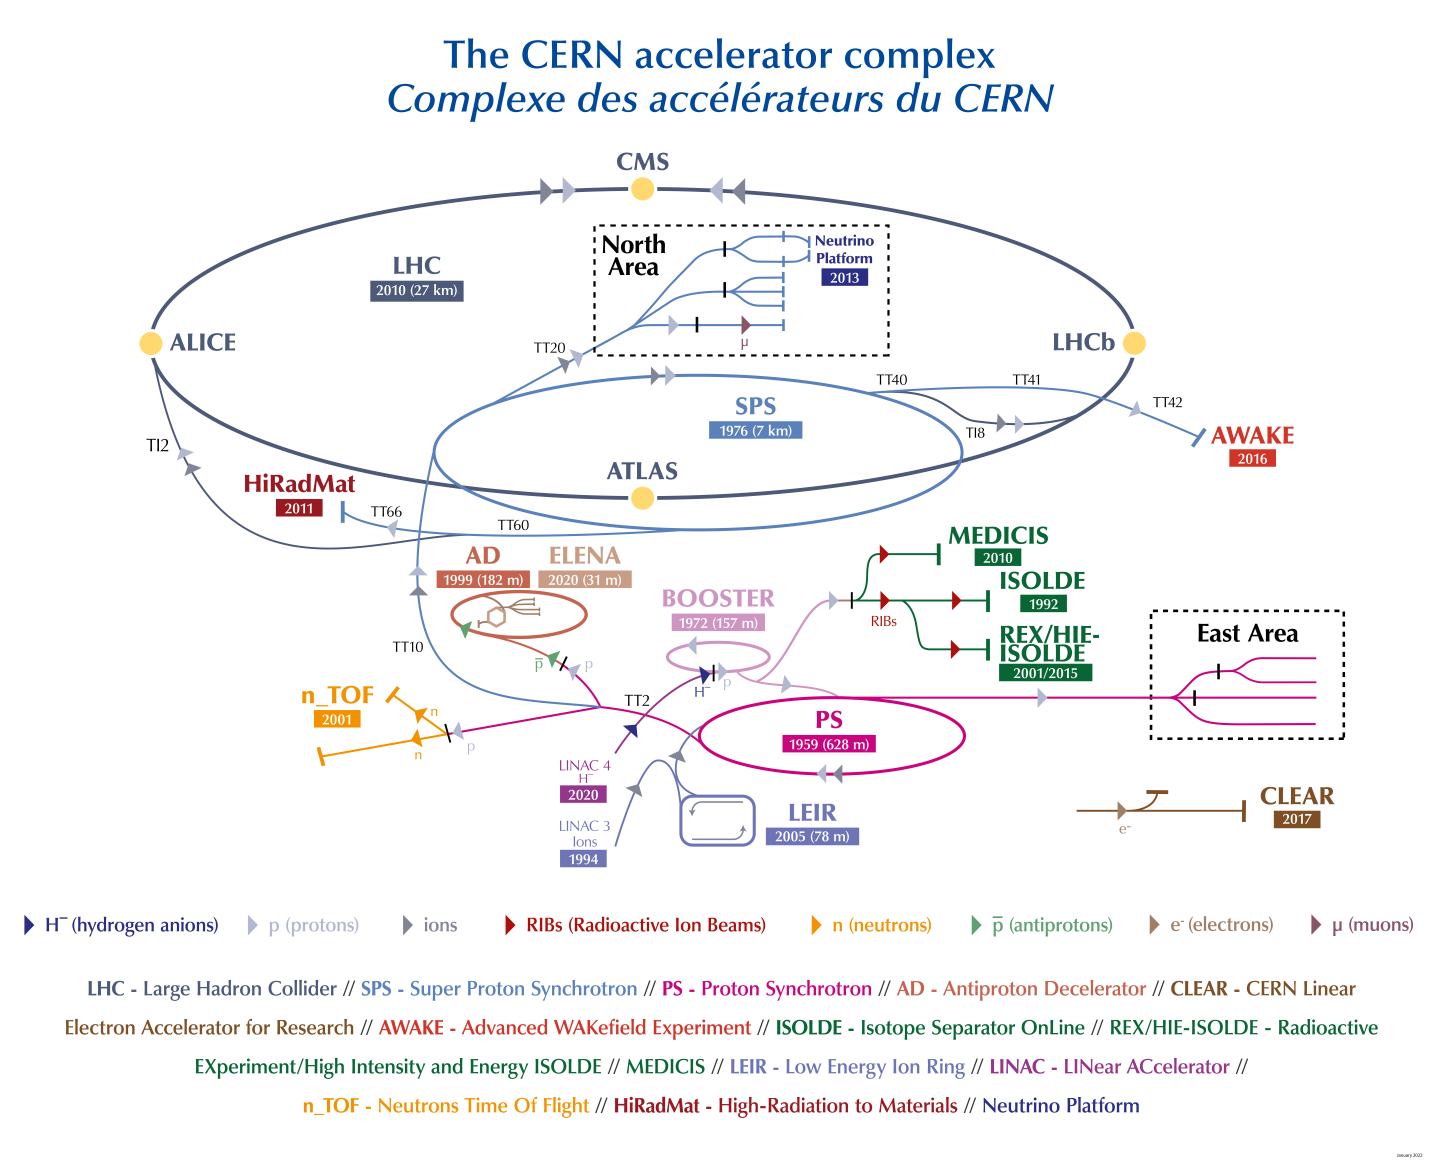
\includegraphics[width=0.8\linewidth]{figures/chapter_II/cern_complex.png}
    \caption{Schematic representation of the CERN accelerator complex.\cite{CERN-complex-2022}}
    \label{fig:cern_complex}
\end{figure}

La cadena comienza con una fuente de gas de hidrógeno, en la que se producen iones de hidrógeno negativos (H$^-$), formados por un protón y dos electrones. Los iones se extraen de la fuente con una energía de $45$ keV y se inyectan en el Linear accelerator (LINAC4), donde un cuadrupolo de radiofrecuencia (RFQ) agrupa los iones en paquetes de partículas y los acelera hasta 3 MeV, tras lo cual una serie de estructuras aceleradoras de radiofrecuencia elevan su energía hasta 160 MeV. A continuación, el haz se inyecta en el Proton Synchrotron Booster (PSB), un sincrotrón formado por cuatro anillos superpuestos, donde una lámina de carbono arranca los dos electrones de cada ion, de forma que a partir de este punto el haz está compuesto únicamente por protones. El PSB acelera los protones hasta 2 GeV antes de transferirlos a la siguiente etapa de la cadena.

Los protones se transfieren después al Proton Synchrotron (PS) donde alcanzan una energía de 26 GeV y donde se define la estructura temporal final del haz: mediante sucesivas divisiones de los paquetes de partículas, se forman trenes de paquetes (\textit{bunches}) separados por 25 ns, que es el espaciado con el que operará posteriormente el LHC. La última etapa previa al LHC es el Super Proton Synchrotron (SPS) que acumula varios trenes procedentes del PS y los acelera hasta 450 GeV, la energía de inyección del LHC.

Desde el SPS, los trenes se transfieren al LHC a través de dos líneas de transferencia independientes, cada una de las cuales llena uno de los dos anillos, de forma que los haces circulan en sentidos opuestos en tubos de vacío separados. Una vez se ha completado el número de paquetes previsto para cada haz, comienza la fase de aceleración gracias a cavidades superconductoras de radiofrecuencia que operan a $400$ MHz. Estas cavidades aportan a los protones del orden de $0.5$ MeV por vuelta y, al mismo tiempo, mantienen los paquetes confinados longitudinalmente. Así, a lo largo de unos veinte minuso, los haces alcanzan su energía final, que durante el Run 3 ha sido de $6.8$ TeV por haz, y una vez estabilizados se hacen colisionar en los cuatro puntos de interacción del anillo.

Estos puntos de intersección están instrumentados con particle detectors installed in underground caverns. "A Toroidal LHC ApparatuS" (ATLAS) and the "Compact Muon Solenoid" (CMS) experiments están situados en los dos diametrically opposite puntos del anillo, y reciben la mayor luminosidad instantánea de colisión. Son los dos general purpose experiments del LHC, diseñados para cubrir un programa de física muy amplio y en gran medida similar. The "LHC beauty" (LHCb) se centra en el estudio de CP-violation y de matter-antimatter asymmetry by studying b quarks physics. "A Large Ion Collider Experiment" (ALICE) is focused mostly on heavy ion collision and quark-gluon plasmas. 



\subsection{LHC Design and parameters}
\label{subsec:LHC_desing}
%
El LHC está instalado en el túnel de $26.7$ km de largo construido to host the LEP collider, por lo que su diseño está en gran parte condicionado por la reutilización de dicho túnel. El diámetro interior del túnel, de apenas $3.7$ m en los arcos, no deja espacio para anillos de imanes separados, por lo que el LHC adopta un diseño \textit{two-in-one}, en el que los dos tubos de vacío por los que circulan los haces en sentidos opuestos, cada uno con sus propias bobinas, se alojan en una misma estructura mecánica y en un mismo criostato.

La energía máxima que puede alcanzar un haz en un anillo de determinada circunferencia viene limitada por el campo magnético capaz de curvar su trayectoria. De esta forma, para mantener en órbita protones de $7$ TeV, el LHC emplea $1232$ dipolos superconductores capaces de generar un campo de $8.33$ T si se enfrían a $1.9$ K, temperatura que se consigue mediante helio superfluido~\cite{Bruning:2004ej}. Además de curvar la trayectoria, es necesario mantener el haz enfocado, para lo que se emplean $392$ cuadrupolos situados a lo largo de todo el anillo junto con imanes de órdenes multipolares superior que se encargan de corregir las imperfecciones del campo. El anillo se divide en ocho arcos, donde se sitúan los dipolos, y ocho secciones rectas, que albergan los puntos de interacción y los sistemas de aceleración, colimación y extracción del haz.

\label{sec:pp_pheno}
Aunque los dos haces de $7$ den lugar a colisiones con energía en el centro de masas de $\sqrt{s}=14$ TeV, la energía disponible para producir nuevas partículas realmente depende de la fracción $x$ delmomento del protón que porte cada uno de sus constituyentes, los partones —quarks y gluones. En consecuencia, la energía efectiva de la interacción es $\sqrt{\hat{s}}=\sqrt{x_1x_2\,s}$, que varía de un suceso a otro, de forma que el LHC explora simultáneamente un amplio rango de energías, y la producción de estados finales pesados, como un par de bosones de Higgs, solo es posible en la fracción de colisiones en que los partones portan una fracción de momento suficiente. El teorema de factorización permite separar la sección eficaz hadrónica QUE TIENE QUE VER AQUI LA SECCION EFICAZ? NO ESTAMOS HABLANDO DE ENERGÍAS? en una parte calculable perturbativamente, la sección eficaz partónica $\hat{\sigma}_{ij}$, y una parte no perturbativa, las funciones de distribución partónica (PDFs) $f_i(x,\mu_F)$, que describen la probabilidad de encontrar en el protón un partón $i$ con fracción de momento $x$~\cite{Collins:1989gx}:
\begin{equation}
    \sigma_{pp\to X} = \sum_{i,j}\int_0^1 dx_1\,dx_2\; f_i(x_1,\mu_F)\,f_j(x_2,\mu_F)\;\hat{\sigma}_{ij\to X}(x_1x_2\,s,\,\mu_R,\,\mu_F).
    \label{eq:factorization}
\end{equation}
Las PDFs no pueden calcularse a partir de primeros principios, sino que se extraen de ajustes globales a datos experimentales~\cite{NNPDF:2017mvq}. Por su parte, la escala de factorización $\mu_F$ y la de renormalización $\mu_R$ no son magnitudes físicas, sino consecuencia del truncamiento de la serie perturbativa, de forma que la dependencia del resultado con ellas refleja los órdenes no calculados. La variación de estas escalas, junto con la incertidumbre de las PDFs, constituye la principal fuente de incertidumbre teórica en la predicción de secciones eficaces, como las de producción de pares de bosones de Higgs discutidas en el Capítulo \ref{ch:theory}.


Dos haces de $7$ TeV dan lugar a colisiones con una energía en el centro de masas de $\sqrt{s}=14$ TeV, pero esta no es la energía disponible para producir nuevas partículas. Los protones no son partículas elementales, por lo que la interacción de interés no se produce entre los protones, sino entre sus constituyentes, los partones —quarks y gluones—, cada uno de los cuales porta una fracción $x$ del momento del protón. En consecuencia, la energía efectiva de la interacción es $\sqrt{\hat{s}}=\sqrt{x_1x_2\,s}$, que varía de un suceso a otro, de forma que el LHC explora simultáneamente un amplio rango de energías, y la producción de estados finales pesados, como un par de bosones de Higgs, solo es posible en la fracción de colisiones en que los partones portan una fracción de momento suficiente. El teorema de factorización permite separar la sección eficaz hadrónica en una parte calculable perturbativamente, la sección eficaz partónica $\hat{\sigma}_{ij}$, y una parte no perturbativa, las funciones de distribución partónica (PDFs) $f_i(x,\mu_F)$, que describen la probabilidad de encontrar en el protón un partón $i$ con fracción de momento $x$~\cite{Collins:1989gx}:

\\

%Los arcos están formados por celdas regulares en las que los dipolos se alternan con los cuadrupolos y los imanes correctores, mientras que las secciones rectas albergan los puntos de interacción y los sistemas de aceleración, colimación y extracción del haz, junto con los cuadrupolos que focalizan los haces antes de cada colisión~\cite{Evans:2008zzb}.

% Luminosidad
El alcance del LHC viene asimismo determinado por la luminosidad instantánea $\mathcal{L}$, que es el parámetro que relaciona el número de sucesos de un proceso dado que se producen por unidad de tiempo y su sección eficaz $\sigma$:
\begin{equation}
    \frac{dN}{dt} = \mathcal{L}\,\sigma .
    \label{eq:event_rate}
\end{equation}
Donde la $\mathcal{L}$ es una magnitud que depende únicamente de las condiciones de los haces. En el LHC, para haces de perfil gaussiano que colisionan con un ángulo de cruce, la luminosidad se expresa como
\begin{equation}
    \mathcal{L} = \frac{\gamma\, f_\text{rev}\, n_b\, N_b^2}{4\pi\, \varepsilon_n\, \beta^*}\, F, \qquad F = \left(1+\left(\frac{\theta_c\,\sigma_z}{2\sigma^*}\right)^2\right)^{-1/2},
    \label{eq:lumi}
\end{equation}
donde $\gamma$ es el factor relativista de los protones, $f_\text{rev}$ la frecuencia de revolución, $n_b$ el número de paquetes por haz, $N_b$ el número de protones por paquete, $\varepsilon_n$ la emitancia transversal normalizada y $\beta^*$ el valor de la función beta en el punto de interacción, que caracteriza el grado de focalización del haz. El factor $F$ da cuenta de la reducción geométrica debida al ángulo de cruce $\theta_c$, y depende del tamaño transversal $\sigma^*$ y longitudinal $\sigma_z$ de los paquetes. Los valores nominales de estos parámetros se recogen en la Tabla \ref{tab:lhc_parameters}.
%
\begin{table}[h!]
    \centering
    \begin{tabular}{l c c}
        \hline
        \textbf{Parameter} & \textbf{Symbol} & \textbf{Nominal value} \\
        \hline
        Beam energy & $E$ & 7 TeV \\
        Revolution frequency & $f_\text{rev}$ & 11.245 kHz \\
        Number of bunches per beam & $n_b$ & 2808 \\
        Protons per bunch & $N_b$ & $1.15\times10^{11}$ \\
        Normalized transverse emittance & $\varepsilon_n$ & 3.75 $\mu$m \\
        Beta function at the interaction point & $\beta^*$ & 0.55 m \\
        Transverse beam size at the interaction point & $\sigma^*$ & 16.7 $\mu$m \\
        Bunch length & $\sigma_z$ & 7.55 cm \\
        Crossing angle & $\theta_c$ & 285 $\mu$rad \\
        Geometric reduction factor & $F$ & 0.836 \\
        Instantaneous luminosity & $\mathcal{L}$ & $10^{34}$ cm$^{-2}$s$^{-1}$ \\
        \hline
    \end{tabular}
    \caption{Nominal LHC parameters for proton-proton collisions~\cite{Bruning:2004ej}.}
    \label{tab:lhc_parameters}
\end{table}

La Ecuación \ref{eq:lumi} muestra cuáles son las vías para aumentar la luminosidad. En primer lugar, la dependencia cuadrática con $N_b$ hace del número de protones por paquete el parámetro más efectivo, y este, junto con la emitancia, viene determinado por la cadena de inyección descrita en la Sección \ref{subsec:LHC_complex}. En segundo lugar, $\beta^*$ puede reducirse focalizando los haces justo antes del punto de interacción, función que desempeñan los cuadrupolos situados a ambos lados de cada experimento. Por último, el número de paquetes está limitado por el espaciado de $25$ ns. Sin embargo, con este espaciado los paquetes de ambos haces se encontrarían también en puntos distintos del de interacción, por lo que los haces deben cruzarse con un pequeño ángulo, lo que reduce la luminosidad a través del factor $F$.\\


Integrando la Ecuación \ref{eq:event_rate} en el tiempo, el número total de sucesos esperado para un proceso es $N=\sigma\int\mathcal{L}\,dt$. La luminosidad integrada, expresada habitualmente en fb$^{-1}$, es por tanto la magnitud que cuantifica el volumen de datos de un análisis, y su medida precisa es imprescindible para convertir un número de sucesos en una sección eficaz. En CMS, esta medida se realiza mediante detectores dedicados, denominados luminómetros, cuya respuesta se calibra en barridos de van der Meer, en los que los haces se desplazan uno respecto al otro para determinar su solapamiento~\cite{CMS:2021xjt}. La precisión alcanzada en cada uno de los años analizados en esta tesis, del orden del porcentaje, se detalla en la Sección \ref{sec:bbtt_systematics}.

% pileup
Sin embargo, con una luminosidad elevada no se produce una única interacción protón-protón por cada cruce de paquetes, sino varias simulaténas, de forma que el número medio de interacciones por cruce viene dado por:
\begin{equation}
    \mu = \frac{\mathcal{L}_b\,\sigma_\text{inel}}{f_\text{rev}},
    \label{eq:pileup}
\end{equation}
donde $\mathcal{L}_b$ es la luminosidad por paquete y $\sigma_\text{inel}$ la sección eficaz inelástica protón-protón. En condiciones nominales, $\mu$ es del orden de 25. Estas interacciones adicionales, conocidas como \textit{pile-up}, son en su inmensa mayoría procesos de baja transferencia de momento que se superponen a la interacción de interés, y a ellas se suman las procedentes de cruces anteriores y posteriores, cuya señal persiste en la electrónica del detector. Por tanto, el pile-up afecta a la reconstrucción de todos los objetos del suceso, y su mitigación constituye uno de los aspectos centrales de los algoritmos descritos en la Sección \ref{sec:POR}. La distribución de $\mu$ registrada por CMS durante el Run 3 se muestra en la Figura \ref{fig:pileup}.


\begin{figure}[h!]
    \centering
    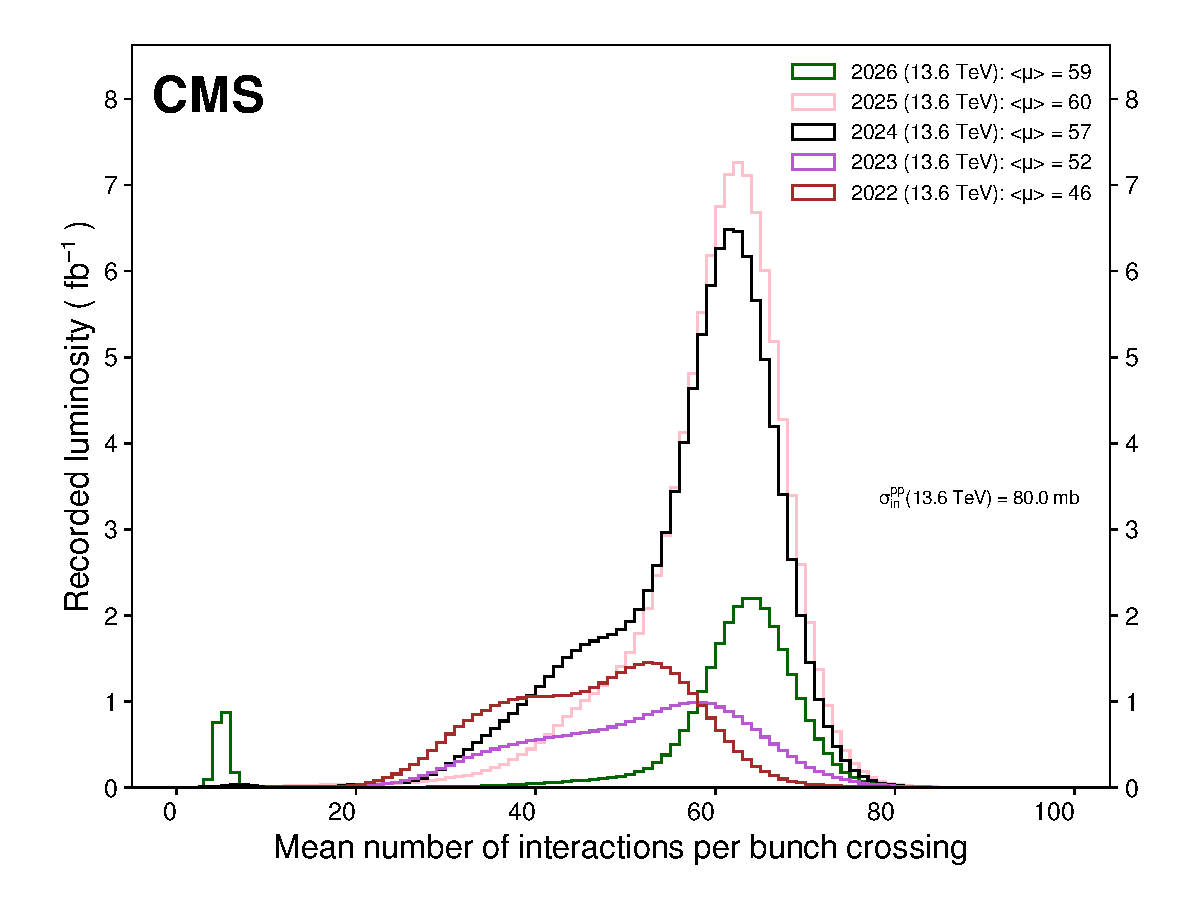
\includegraphics[width=0.75\linewidth]{figures/chapter_II/pileup_run3.pdf}
    \caption{Distribution of the mean number of interactions per bunch crossing recorded by CMS in proton-proton collisions during each year of Run 3, computed assuming an inelastic cross section of 80 mb~\cite{TOTEM:2017asr}. The mean value $\langle\mu\rangle$ of each year is indicated~\cite{CMS-LumiPublicResults}.}
    \label{fig:pileup}
\end{figure}






CIERRE DE LO QUE ME ABRE CADA PARAMETRO

The LHC is installed in a 26.7 km long tunnel built between 1984 and 1989 to host the
CERN Large Electron Positron (LEP) collider. The tunnel is located in the region nearby
Geneva and extends across the French and the Swiss borders. In the LHC, two separate,
counter-rotating particle beam lines are kept in orbit in two magnetic channels thanks to
44 Chapter 2. Experimental apparatus
the field generated by superconduting niobium-titanium coils. The particles are steered
by a magnetic field of 8.3T generated by a current of about 11 kA in the 1232 dipole
magnets, each measuring 15 metres of length and 35 tonnes of weight. The stability of
the beam dynamics is ensured by 392 quadrupoles magnets measuring 5 to 7 metres of
length, that focus the particles and keep them in a narrow beam. Special quadrupoles
are installed in front of the collision points to squeeze the beams and increase the proton
density in the collisions. Superconducting magnets are cooled with superfluid helium-4
and kept to a working temperature of 1.9K.

The LHC ring is made of eight 2.45km long arcs, where bending dipoles are placed, and
and eight 545m long straight sections. Because the tunnel is inherited from LEP, the
LHC design faces some space limitations: in the arcs, for instance, the tunnel has small
internal diameter of 3.7 m. Therefore, instead of implementing separate rings of magnets
for each of the beams, the two counter-rotating beamlines need to be hosted within a
single cryogenic and mechanic assembly; the antiparallel magnetic fields are generated
by two independent sets of coils, although they are are placed close enough to each other
that they are coupled both magnetically and mechanically.
The LHC electromagnets are made of copper-clad niobium-titanium superconductor,
amounting globally to about 470 tonnes. The beams are kept on their circular path
through the magnetic field of 1232 dipoles operating at 8.33 T, while 392 quadrupole
magnets keep the particles focused in narrow beams. Dedicated quadrupoles squeeze
the beams in proximity of the interaction points and magnets of higher multipole orders
correct smaller imperfections in the magnetic field. The operating temperature of the
magnets is 1.9 K (-271.25C); approximately 96 tonnes of superfluid helium-4 are needed
to keep them cool.

kept travelling in opposite directions before colliding in the designated
interaction points once they have reached a target energy; although the design center-ofmass
energy for proton-proton collisions is ps = 14TeV, the target energy of the LHC
acceleration stage changed over the research phases, as detailed in Sec. 2.1.4: 3.5TeV
until 2011, 4 TeV in 2012, 6.5 TeV from 2015 on.

Luminosity


\subsection{Operation}

The accelerator is a 27 km circular collider built around
100 m underground composed by two rings where two beams of protons or heavy
ions circulate in opposite directions inside vacuum pipes. The beams are bended
using 1232 superconducting dipoles, cooled down with super
uid helium to 1.9 K,
which generate an 8.3 T magnetic eld. To focus the beams and avoid spreading,
392 quadrupole magnets are used

The LHC is the last step of the accelerating chain in which the particles reach
the operating energies. The CERN accelerator complex is shown in Fig. 2.1. At the
beginning of the chain, hydrogen atoms are ionized and injected into the LINAC2,
where they are accelerated to an energy of around 50 MeV. Then, the beam is passed
through a series of circular synchrotrons, reaching 1.4 GeV after the BOOSTER,
26 GeV after the PS and 450 GeV after the SPS, before they enter into the LHC
and reach their target energy. The designed center-of-mass energy (ps) for protonproton
collisions is 14 TeV, although the target energy has changed over the different
phases: 7 TeV during 2010 and 8 TeV during 2011 and 2012 (3-year period called
Run 1), 13 TeV during Run 2 (2015-2018) and 13.6 TeV during Run 3 (which started
in 2022).

The accelerator complex at CERN is a succession of machines that accelerate particles to increasingly higher energies to uncover the mysteries of the Universe. Each machine or accelerator boosts the energy of a beam of particles, before injecting the beam into the next machine in the sequence. In the Large Hadron Collider (LHC) – dark blue line – particle beams are accelerated up to the record energy of 6.5 TeV per beam. Most of the other smaller accelerators in the chain have their own experimental halls where beams are used for experiments at lower energies.


Protons are progressively accelerated by Linac4 (purple), PS Booster (pink), PS (magenta), SPS (blue), and ultimately at the LHC (dark grey). The proton beams circulated through the LHC collide in the center of the four particle detectors (yellow dots): ATLAS, ALICE, CMS, and LHCb



- Schema CERN: accelerator complex (experiments)
- design parameters: luminosity
- operation and plan




\section{The CMS Experiment}
\label{sec:CMS}
\subsection{Coordinate system and proton-proton collision phenomenology}
%junto o por separado estas dos secciones?
\subsection{Detector structure (subdetectors)}
\subsection{CMS Trigger System}
\subsection{Data Acquisition and Computing systems}
%??? añadir esta subsection? o no me hace falta?






\section{CMS physics objects reconstruction}
\label{sec:POR}
\subsection{The Particle Flow algorithm}
\subsection{Final state particle reconstruction}
\label{subsec:Finalstate}
\subsection{Muon}
%... ver como me cuadra mas
\subsubsection{Muon}
\subsubsection{Hadronic \texorpdfstring{$\tau$}{τ} leptons}
\label{subsec:Taus}
\noindent The $\tau$-lepton is the heaviest lepton in the SM, with a mass of $1.777$ GeV. It is the only lepton that can decay both leptonically and hadronically, with a short lifetime of $2.9\times 10^{-13}$ s. Leptonic decays account for about $35\%$ of the $\tau$-lepton decay width, while hadronic decays account for approximately $64.8\%$, as shown in Table \ref{tab:tau_decays}, which reports the corresponding branching fractions. In all decays, neutrinos remain undetected, and it is not possible to measure the momentum of the decaying $\tau$ with exact precision.

\begin{table}[h!]
    \centering
    \begin{tabular}{l c}
        \hline
        \textbf{Decay Mode} & \textbf{BR (\%)} \\
        \hline
        \multicolumn{2}{l}{\textbf{Leptonic decays}} \\
        $\tau^- \to e^- \,\bar{\nu}_e\, \nu_\tau$ & 17.8 \\
        $\tau^- \to \mu^- \,\bar{\nu}_\mu\, \nu_\tau$ & 17.4 \\
        \hline
        \multicolumn{2}{l}{\textbf{Hadronic decays}} \\
        $\tau^- \to h^- \nu_\tau$ & 11.5 \\
        $\tau^- \to h^- \pi^0 \nu_\tau$ & 25.9 \\
        $\tau^- \to h^- \pi^0 \pi^0 \nu_\tau$ & 9.5 \\
        $\tau^- \to h^- h^+ h^- \nu_\tau$ & 9.8 \\
        $\tau^- \to h^- h^+ h^- \pi^0 \nu_\tau$ & 4.8 \\
        \textit{Other} & 3.3 \\
        \hline
    \end{tabular}
    \caption{Decay modes of the $\tau$ lepton and corresponding branching fractions (BR) in $\%$; the charged hadrons are denoted by h$^{\pm}$}
    \label{tab:tau_decays}
\end{table}


In the leptonic decay mode, the lepton is accompanied by two neutrinos and is reconstructed simply as the corresponding electron or muon following the standard procedures describes in the previous sections, along with the to neutrinos emitted along the $\tau$-lepton flight direction. While neutrinos do not leave a direct trace upon escaping the detector, they do generate a momentum imbalance in the transverse plane. By measuring the missing transverse momentum in the event, their presence can be inferred. Therefore, the main challenge in identifying such decays lies in reconstructing and measuring the missing transverse momentum (MET), which serves as an indirect measurement of neutrinos, as described in Section \ref{sec:MET}. In addition, the energy fraction of the decaying $\tau$-lepton carried by the electron or muon falls within a continuous spectrum, which makes it difficult to distinguish between leptonic $\tau$ decays and prompt leptons. These effects makes the identification and reconstruction of $\tau$ leptonic decay a particularly challenging task.

Nevertheless, since leptonic decays are reconstructed based on the corresponding light lepton, discussing the reconstruction of $\tau$ leptons implicitly refers to hadronic $\tau$ ($\tau_h$) reconstruction. Hadronic decay can occur either directly or via intermediate resonances such as $\rho$(770) or $a_1$(1260), resulting in a variety of charged and neutral hadrons. Due to charge conservation, the decay products include and odd number of charged hadrons, typically one or three, which are reconstructed as hadron jets and a neutrino $\nu_{\tau}$. Due to the high particle multiplicity in hadronic $\tau$ decays, a reliable reconstruction algorithm must be able to identify the PF candidates associated with the charged hadrons, as well as the photons originating from $\pi^0$ decay; group them to determine the decay mode; and determine the kinematic properties of the $\tau_h$. To meet these requirements, the reconstruction of hadronically decaying $\tau$ leptons is operated in CMS with the Hadron-Plus-Strips (HPS) algorithm {\color{red}[\ref{}]}.

The HPS algorithm is employed to identify and reconstruct $\tau_h$ candidates by verifying the compatibility of all PF jet candidates with a $\tau$-lepton. To this end, the HPS algorithm is seeded by the AK4 PF jet candidates reconstructed as in Section \ref{sec:Jet}, and for each seeding jet, all particles within a cone of radios $\Delta R<0.5$ around the jet axis are tested as hadron candidates or clusters of electron and photon candidates originating form neutral pions decays (photons from $\pi^0$ decays may convert into electron-positron pairs). These reconstructed objects are referred to as \textit{strips}, and their reconstruction is performed iteratively: candidates within the clustering region around each strip are progressively added, and the strip position is recomputed using a $p_T$-weighted average. The $\eta \times \varphi$ window is dynamically adjusted in each iteration to adapt to the strip $p_T$ and ensure optimal energy collection. This procedure is repeated until no further candidates are found. At this stage, the HPS algorithm combines both charged hadrons and strips inside the PF jet to form all the possible combinations of hadrons for the various decay modes (listed in Table \ref{tab:tau_decays}): h$^{\pm}$, h$^{\pm}\pi^0$, h$^{\pm}\pi^0\pi^0$, h$^{\pm}$h$^{\mp}$h$^{\pm}$ and h$^{\pm}$h$^{\mp}$h$^{\pm}\pi^0$ (plus the additional $\nu_{\tau}$). Each decay mode hypothesis includes additional quality and invariant mass requirements to ensure it aligns with a genuine $\tau_h$. Among all candidates within a seed region, the hadronic $\tau_h$ with the highest $p_T$ is selected.

One of the major challenges in the $\tau_h$ reconstruction lies in accurately distinguishing genuine $\tau$ leptons from misidentified objects, such as background events involving QCD multi-jet production. To enhance the purity of the hadronic $\tau$ reconstruction, a convolutional neural network (CNN), the \textsc{DeepTau} identification method {\color{red}[\ref{}]}, has been adopted in CMS analyses since the end of the LHC Run 2 as a tool to discriminate real $\tau_h$ from quark and gluon jets, as well as from electrons and muons. This machine learning (ML)-based algorithm integrates information from high-level reconstructed $\tau_h$ features, the decay mode extracted from the HPS algorithm and low-level data used to construct the PF candidates. The \textsc{DeepTau} algorithm defines three different discriminators, each targeting a specificy type of background: jets \textsc{DeepTauVSjet}, electrons \textsc{DeepTauVSe}, and muons \textsc{DeepTauVSmu}. Each discriminator has a different set of working points (WP). 

Although the origins of this identification method date back to Run 2, the \textsc{DeepTau} algorithm received major updates at the start of Run 3. This new version includes upgrades such as reducing discrepancies between data and simulation in regions of high hadronic purity by integrating domain adaptation techniques, and improving data handling, resulting in overall enhanced performance. The \textsc{DeepTau} algorithm has been shown to achieve a significant improvement in the identification and reconstruction of $\tau_h$ compared to previous algorithm. {\textcolor{red}{Figure illustrates this enhancement for the three discriminators.}}

For example, for a given jet rejection level, the efficiency for genuine tau h candidates is increased by 10–30%.

A further advancement in Run 3 pertains to boosted topologies. When $\tau$ leptons are produced by highly boosted resonances, their decay products become collimated within a narrow cone, often forming a single jet, similar to the behavior observed for AK8 jets. While no dedicated reconstruction existed in Run 2, an extension of the HPS algorithm has been developed for Run 3 to target high-momentum candidates by exploiting the jet substructure of the $\tau_h$ candidates. The algorithm reverses the final step in the clustering sequence that forms the large-radius jet to identify two sub-jets that are compatible with the expected topology of boosted $\tau$ decay. Specific requirements are in place to suppress misidentification with quark-gluon jets, electrons or muons. This approach has been shown to outperform the standard HPS for highly boosted $\tau$ leptons while maintaining optimal misidentification rates. The selected boosted $\tau$ candidates are then passed to the HPS algorithm for standard $\tau$ reconstruction.


Hadronically decaying tau leptons are key elements for analysis involving complex final states, such as the $HH\rightarrow bb\tau\tau$ analysis, where robust $\tau$ reconstruction plays a central role. Accurate and reliable reconstruction and identification of $\tau$ leptons are essential, as the performance of the algorithms described in this section directly impacts the sensitivity to such signatures. Therefore, their validation becomes a crucial component of this work, which will focus on a detailed assessment of the identification algorithms used in Run-3 and its performance across the 2022-2026 data-taking periods in Chapter \ref{ch:Tau}.







\section{Trigger???}
\label{sec:TRG}

  \part{Search for Higgs boson pair production in the bb\texorpdfstring{$\tau\tau$}{ττ} final state}
  \chapter{The \texorpdfstring{$\tau_h$}{τh} identification algorithms and their performance}
\label{ch:Tau}
%
The precise and accurate reconstruction of $\tau$ leptons is a crucial part of the $HH\rightarrow bb\tau\tau$ analysis covered in Chapter \ref{ch:bbtt_analysis}. Furthermore, a significant number of physics analyses — such as measurements of Higgs boson production~\cite{CMS-HIG-16-043,CMS-HIG-19-010} and of the \CP structure of its Yukawa coupling to $\tau$ leptons~\cite{CMS-HIG-20-006}, and searches for new physics in final states with $\tau$ leptons~\cite{CMS-HIG-21-001,CMS-PAS-EXO-24-012,CMS-PAS-EXO-24-020} — rely on the adequate identification of $\tau$ decay products and their properties. This broad physics program necessitates continuous development of reconstruction and identification techniques, which in CMS for $\tau$ leptons are coordinated within the Tau Physics Object Group (Tau POG). A central component of the study of $\tau$ leptons, which will be emphasized subsequently, involves validating the applied techniques to ensure their correct behavior in data.

In CMS, the reconstruction and identification of hadronic $\tau$ leptons constitute two complementary steps. The reconstruction stage, performed by the HPS algorithm~\cite{CMS-TAU-14-001} (see Section \ref{subsec:Taus}), assembles the visible decay products into a $\tau_h$ candidate and determines its decay mode and kinematic properties. The identification step then classifies these reconstructed candidates as a genuine $\tau$ lepton or as a misidentified jet, electron or muon.

This chapter provides a detailed examination of the identification of hadronic $\tau$ leptons. Section \ref{sec:Tau_MisID} lays the groundwork and emphasizes the challenges associated with distinguishing genuine $\tau_h$ candidates from background objects, Section \ref{sec:DeepTau2.5} summarizes the identification algorithms and compares their performance, and Section \ref{sec:Tau_validation} presents their validation with the data recorded by CMS from 2022 to 2026. This validation is the contribution of this thesis to the Tau POG, and its results with the 2024 and 2025 data have been published in Ref.~\cite{CMS-DP-2025-074}.


\section{Challenges in \texorpdfstring{$\tau_h$}{τh} identification}
\label{sec:Tau_MisID}
%
As described in Section \ref{subsec:Taus}, the HPS algorithm is configured to prioritize the reconstruction efficiency of genuine $\tau_h$, which exceeds $80\%$ for $p_T > 30$ GeV and approaches $90\%$ above $100$ GeV~\cite{CMS-TAU-20-001}. Therefore, it inevitably suffers from contamination by other processes, meaning that a fraction of reconstructed $\tau_h$ candidates originates from objects that mimic the topology of hadronic $\tau$ decay. The dominant source of misidentification arises from jets, since the HPS algorithm is seeded by PF jets that can reproduce the charged-track multiplicity and electromagnetic signature characteristic of $\tau$ decays, i.e., a highly collimated quark or gluon jet can resemble a $\tau$ decay, as illustrated in Figure \ref{fig:tau_fakes}. Light leptons can also be misidentified as $\tau$ leptons. A muon can mimic a one-prong decay when it deposits a significant fraction of its energy in the calorimeters, while an electron can be taken as the charged hadron of the decay, with the photons it radiates through bremsstrahlung clustered into a strip, which reproduces the signature of a h$^{\pm}\pi^0$ decay. These signatures are also illustrated in Figure \ref{fig:tau_fakes}.
%
% \begin{figure}[h!]
% \centering
% \begin{subfigure}[t]{0.48\linewidth}
%   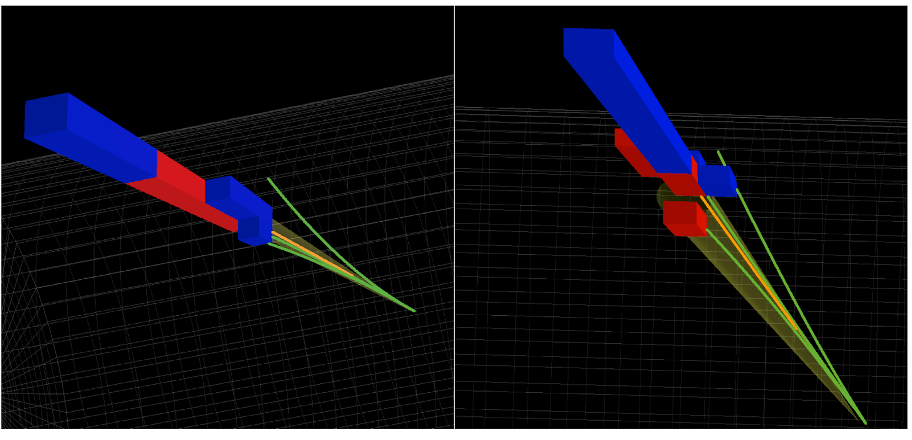
\includegraphics[width=1\linewidth]{figures//chapter_III/tau_jet_sim.png}
%     \caption{Simulation of a $\tau_h$ decay into h$^{\pm}$h$^{\mp}$h$^{\pm}\pi^0$ (left) and of a collimated jet resembling a $\tau_h$ (right) in the CMS detector.}
%     \label{fig:tau_jet_sim}  
% \end{subfigure}
% \hfill
% \begin{subfigure}[t]{0.48\linewidth}
%     \centering
%     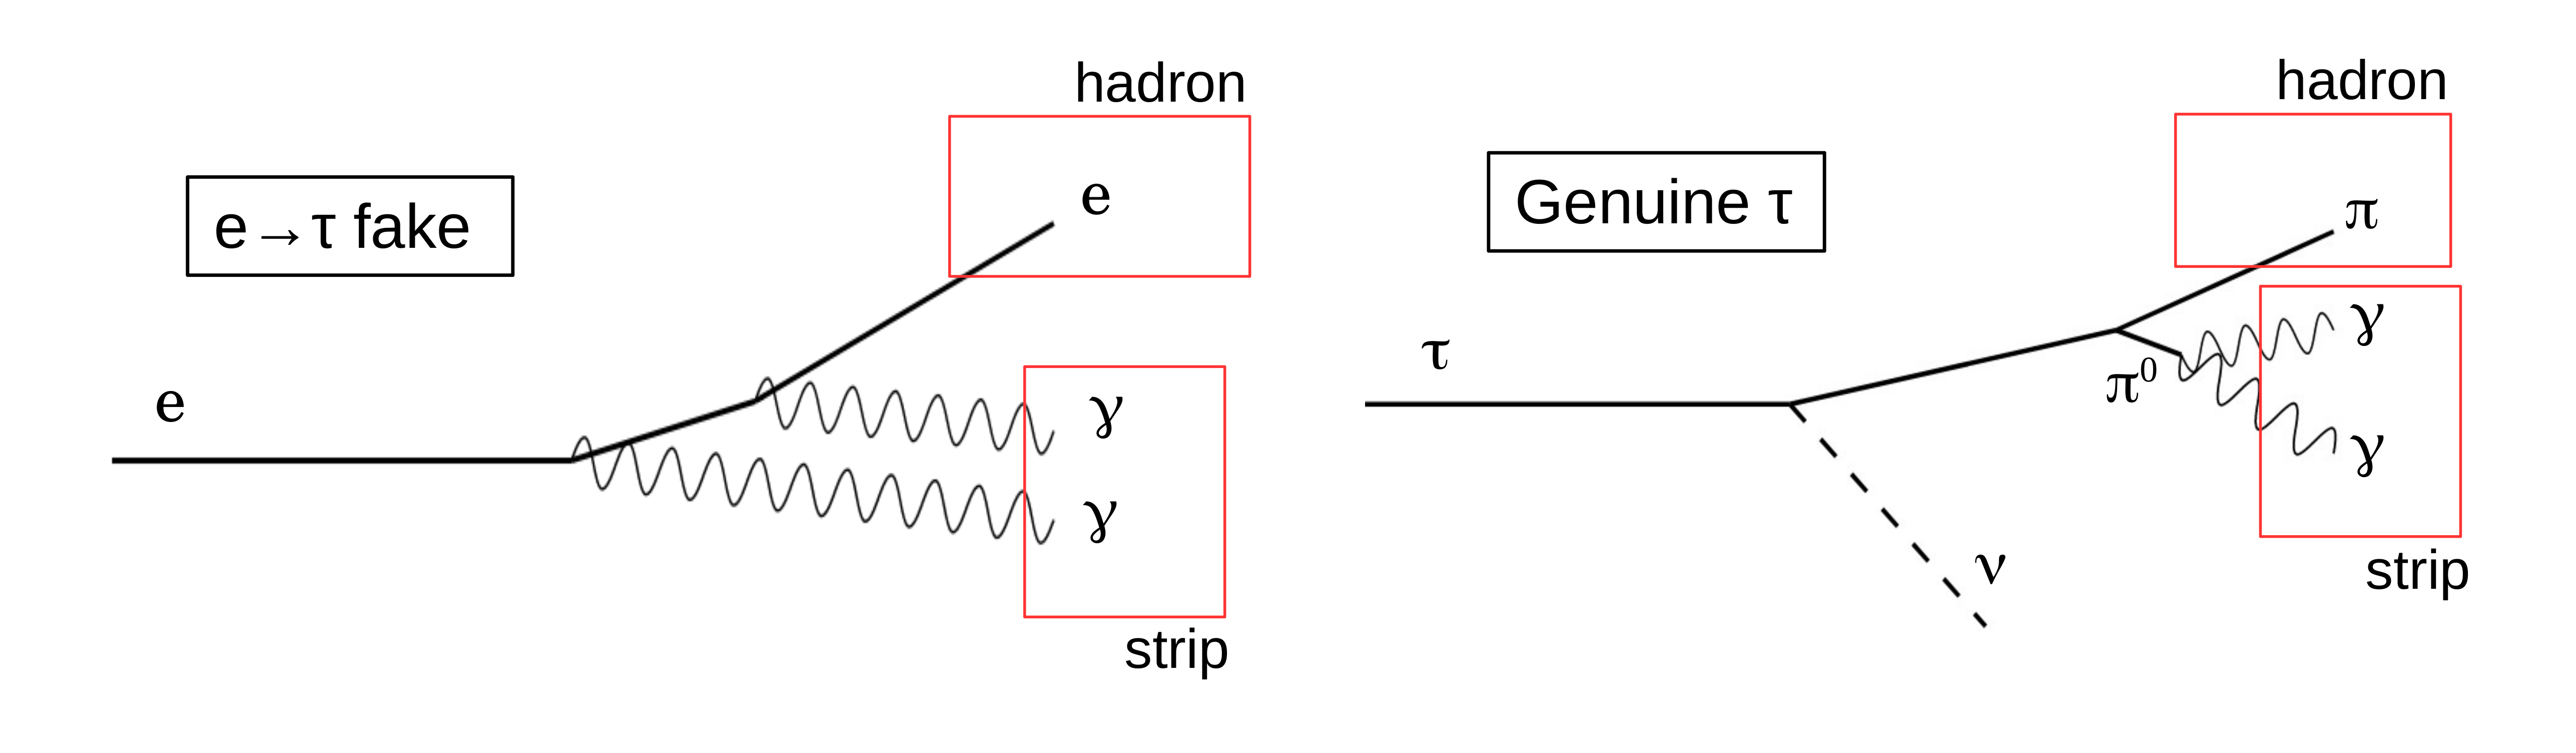
\includegraphics[width=1\linewidth]{figures//chapter_III/electron_faking_tau.png}
%     \caption{Schematic representation of the signatures identified by the HPS algorithm for an electron faking a $\tau_h$ (left) and a genuine $\tau_h$ (right). \textcolor{red}{hacer más grande esta figura}}
%     \label{fig:ele_fake_tau}
% \end{subfigure}
% \caption{Examples of objects misidentified as $\tau_h$ candidates by the HPS algorithm}
% \label{fig:tau_fakes}
% \end{figure}
\begin{figure}[h!]
    \centering
    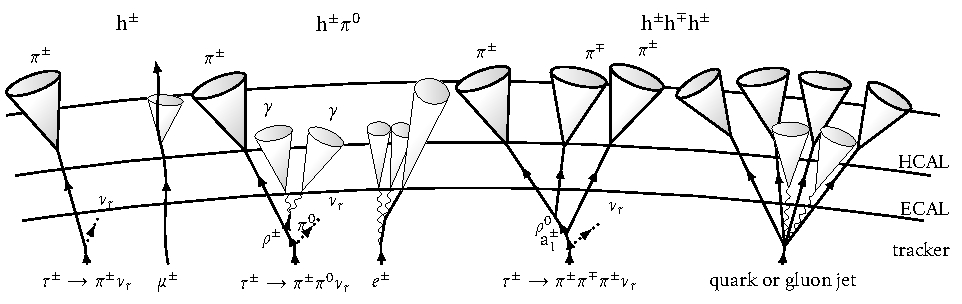
\includegraphics[width=\linewidth]{figures/chapter_III/tau_fakes_tikz.pdf}
    \caption{Signatures of genuine $\tau_h$ decays and of the objects that the HPS algorithm can reconstruct in the same decay mode, indicated above each pair. From left to right, a one-prong decay and a muon that deposits part of its energy in the calorimeters, a one-prong decay with a neutral pion and an electron whose bremsstrahlung photons are clustered into a strip and whose shower reaches the HCAL, and a three-prong decay and a quark or gluon jet, which usually contains more particles spread over a wider angle. Adapted from Ref.~\cite{Neutelings:tau_decay}.}
    \label{fig:tau_fakes}
\end{figure}

The reconstruction of genuine $\tau_h$ has its own limitations. Depending on the decay mode, between $11\%$ (h$^{\pm}$) and $25\%$ (h$^{\pm}\pi^0$) of the generated $\tau_h$ are not reconstructed in any of the HPS decay modes, mainly because the tracks of charged hadrons are reconstructed with an efficiency of about $90\%$~\cite{CMS-TAU-20-001}. Part of the three-prong decays in which one track is lost are recovered as two-prong candidates, but their charge is correctly assigned in only about $70\%$ of the cases, compared with $99\%$ for the other decay modes~\cite{CMS-TAU-20-001}, which is why they are not among the four decay modes used in analyses (Figure \ref{fig:tau_DMs}). These candidates, lost or misreconstructed by HPS, are one of the motivations for the identification algorithms that do not depend on it, presented in Section \ref{subsec:PNet}.

These effects reflect the challenges associated with the complex topology of hadronic $\tau$ decays, and highlight the need for a dedicated identification step to improve the purity of reconstructed $\tau_h$ candidates. To this end, various methods have been implemented in CMS over the years, ranging from cut-based isolation sum discriminators and Boosted Decision Tree discriminator~\cite{CMS-TAU-14-001,CMS-TAU-16-003} to more sophisticated deep learning-based algorithms, described in the following section.


\section{The \texorpdfstring{$\tau_h$}{τh} identification algorithms}
\label{sec:DeepTau2.5}
%
Given the aforementioned reconstruction limitations, a dedicated identification approach is needed. The challenge of discriminating between the reconstructed $\tau_h$ candidates, given the large number of correlated observables involved in this type of task, has led to the adoption of advanced deep learning techniques capable of fully exploiting the available information and ensure robust performance across different data-taking conditions. 

The \textsc{DeepTau} neural network-based algorithm was deployed at the end of Run 2, and has since become the standard $\tau_h$ identification method in CMS. The first version v2.1~\cite{CMS-TAU-20-001} was presented initially, and was then upgraded to v2.5~\cite{CMS-TAU-24-001} during the early Run 3 period, introducing major improvements that will be briefly discussed next. In parallel, alternative identification strategies for genuine $\tau_h$ candidates are being explored, leveraging modern architectures such as graph neural networks (\textsc{PNet}) and transformers (\textsc{UParT}) to treat $\tau_h$ candidates within a broader jet classification framework.



\subsection{The \textsc{DeepTau} algorithm}
\label{subsec:DeepTau}
%
\textsc{DeepTau} is a convolutional neural network that classifies each $\tau_h$ candidate reconstructed by HPS as a genuine $\tau_h$, a quark or gluon jet, an electron or a muon, so that the three discriminations described in Section \ref{sec:Tau_MisID} are performed by a single network~\cite{CMS-TAU-20-001,CMS-TAU-24-001}. To do so, it combines two types of information. The first is a set of high-level variables that describe the candidate as a whole, such as its kinematics, its isolation, or the compatibility of its tracks with the primary vertex. The second is the set of all particles reconstructed around the candidate, whose individual properties are arranged in two grids in the $\eta$-$\phi$ plane centered on the $\tau_h$ axis, an inner grid covering the region of the decay products and a wider outer grid that captures the surrounding activity, which is larger for jets than for genuine $\tau_h$. The input variables of both types are summarized in Table \ref{tab:deeptau_inputs}.
%
\begin{table}[h!]
    \centering
    \begin{tabular}{l l}
        \hline
        \textbf{Input block} & \textbf{Variables} \\
        \hline
        \multicolumn{2}{l}{\textit{High-level features ($43$ variables)}} \\
        $\tau_h$ candidate & $p_T$, $\eta$, energy, charge, number of charged and neutral constituents \\
        Isolation          & energy sums of the different particle types around the candidate \\
        Lifetime           & impact parameters of the leading track, properties of the SV \\
        Strips             & spread in $\eta$ and $\phi$ of the energy in the strips \\
        Electron rejection & calorimeter variables discriminating against electrons \\
        Pileup             & pileup energy density $\rho$ \\
        \hline
        \multicolumn{2}{l}{\textit{Low-level features (inner and outer grids around the $\tau_h$ axis)}} \\
        Particle types     & PF electrons, muons, photons, charged and neutral hadrons, \\
                           & standalone electrons and muons \\
        Kinematics         & $p_T$, $\Delta\eta$ and $\Delta\phi$ with respect to the $\tau_h$ axis, charge \\
        Tracks             & track quality, compatibility with the PV or an SV \\
        Detector deposits  & ECAL and HCAL energy, muon station hits \\
        Pileup             & PUPPI weight \\
        \hline
    \end{tabular}
    \caption{Summary of the input features used by the \textsc{DeepTau} v2.5 algorithm~\cite{CMS-TAU-24-001}.}
    \label{tab:deeptau_inputs}
\end{table}

This set of input information is processed by a combination of dense and convolutional layers, and the final layer of the network acts as a multiclass classifier~\cite{CMS-TAU-20-001}, providing the probabilities that the reconstructed $\tau_h$ candidate corresponds to a genuine $\tau_h$, an electron, a muon, or a quark or gluon jet. From these probabilities, three discriminators are built, one against each type of background (\textsc{VSjet}, \textsc{VSe}, \textsc{VSmu}), by comparing the probability of the genuine $\tau_h$ class with that of the corresponding background. Each discriminator has its own set of working points, defined by the efficiency for genuine $\tau_h$, as described in Section \ref{subsec:Taus}. 

% This set of input information is processed by a combination of dense and convolutional layers, and the final layer of the network acts as a multiclass classifier~\cite{CMS-TAU-20-001}, providing the probabilities that the reconstructed $\tau_h$ candidate corresponds to a genuine $\tau_h$, an electron, a muon, or a quark or gluon jet. From these probabilities, three discriminators are built, one against each type of background (\textsc{VSjet}, \textsc{VSe}, \textsc{VSmu}), defined as
% \begin{equation}
%     D_\alpha = \frac{y_\tau}{y_\tau + y_\alpha}, \qquad \alpha \in \{e,\,\mu,\,\text{jet}\},
%     \label{eq:deeptau_discriminant}
% \end{equation}
% %
% where $y_\tau$ and $y_\alpha$ are the probabilities assigned to the genuine $\tau_h$ class and to the background class $\alpha$, so that $D_\alpha$ approaches unity for genuine $\tau_h$. Each discriminator has its own set of working points, defined by the efficiency for genuine $\tau_h$, as described in Section \ref{subsec:Taus}.
As already mentioned, two versions of \textsc{DeepTau} have been used in CMS. The first, v2.1, was introduced at the end of Run 2 and trained exclusively on simulated events. Its successor, v2.5, used in Run 3 and in the analysis presented in this thesis, keeps essentially the same architecture, but was retrained with a larger and more balanced dataset, optimized hyperparameters and a revised set of inputs. As shown in Figure \ref{fig:DeepTau_versions}, the probability for jets to be misidentified as $\tau_h$ is reduced by $30$–$50\%$ over the whole efficiency range, the rejection of electrons improves mainly for the tightest working points, where the misidentification probability is reduced by almost a factor of two, and the rejection of muons remains unchanged.
%
\begin{figure}[h!]
    \centering
    \begin{subfigure}[t]{0.32\linewidth}
        \centering
        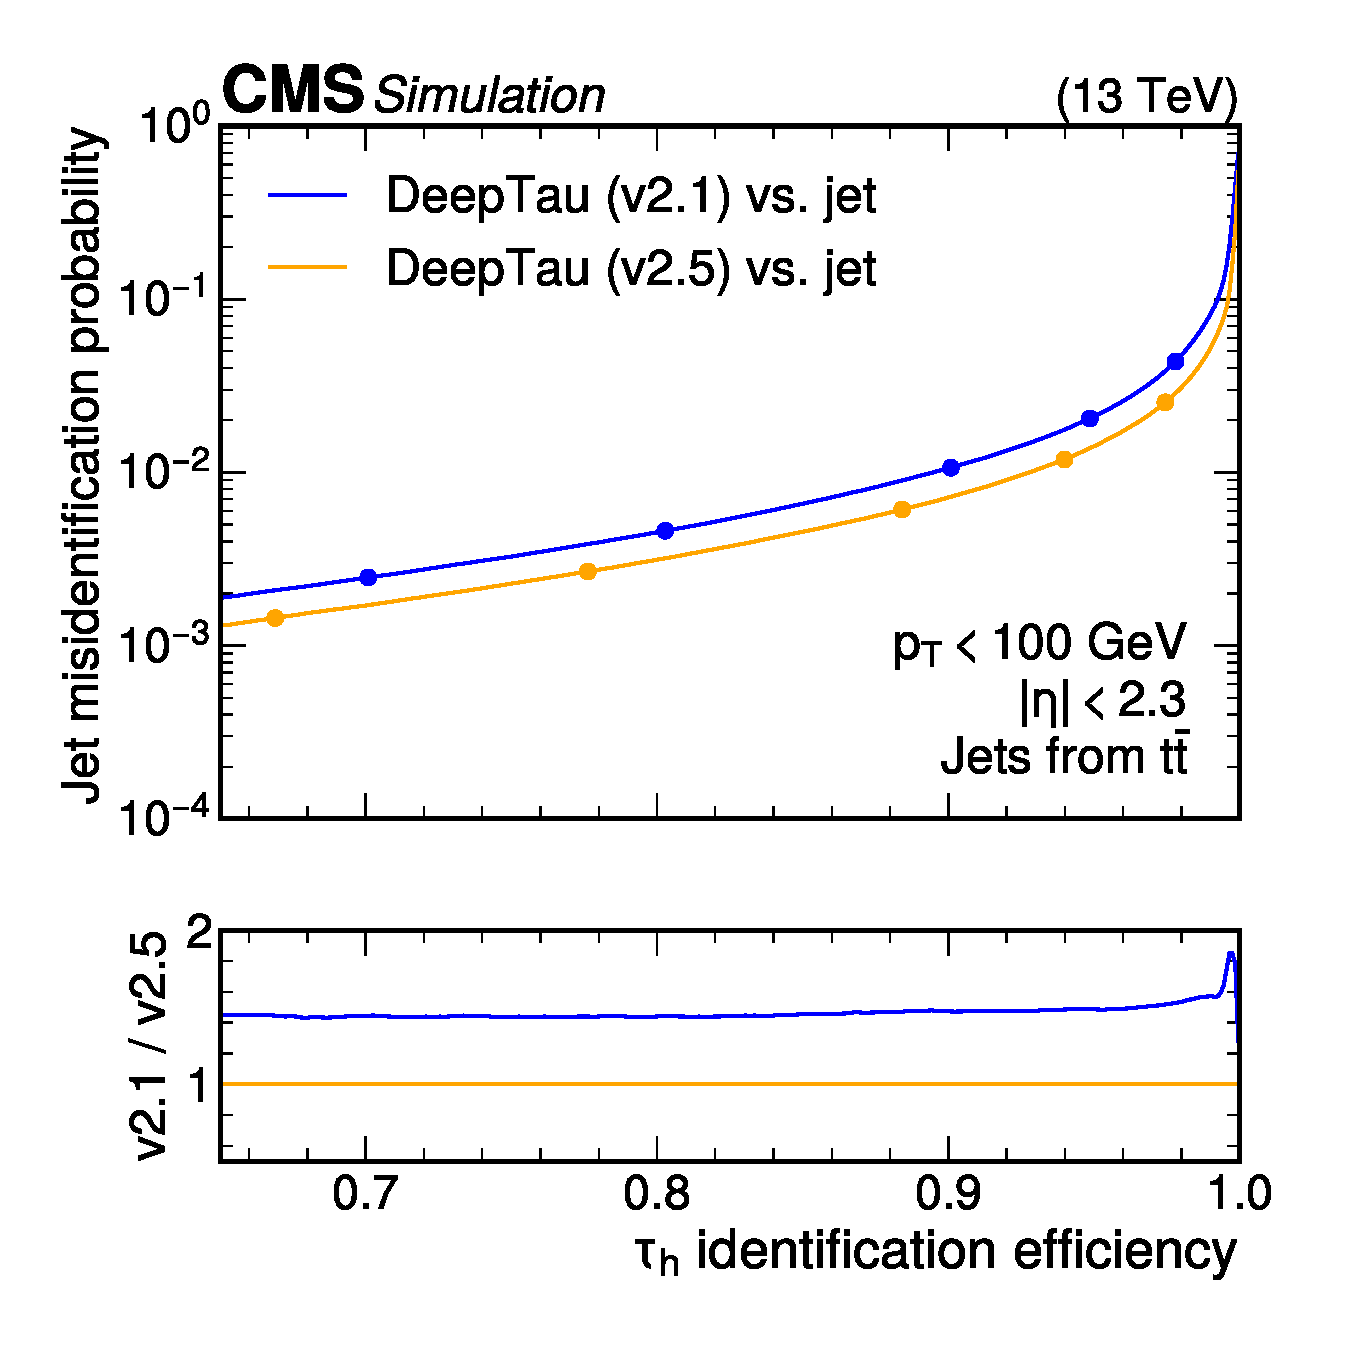
\includegraphics[width=\linewidth]{figures/chapter_III/CMS-TAU-24-001_Figure_006-a.pdf}
        \caption{\textsc{VSjet}}
        \label{fig:DeepTau2p5VSjet}
    \end{subfigure}
    \hfill
    \begin{subfigure}[t]{0.32\linewidth}
        \centering
        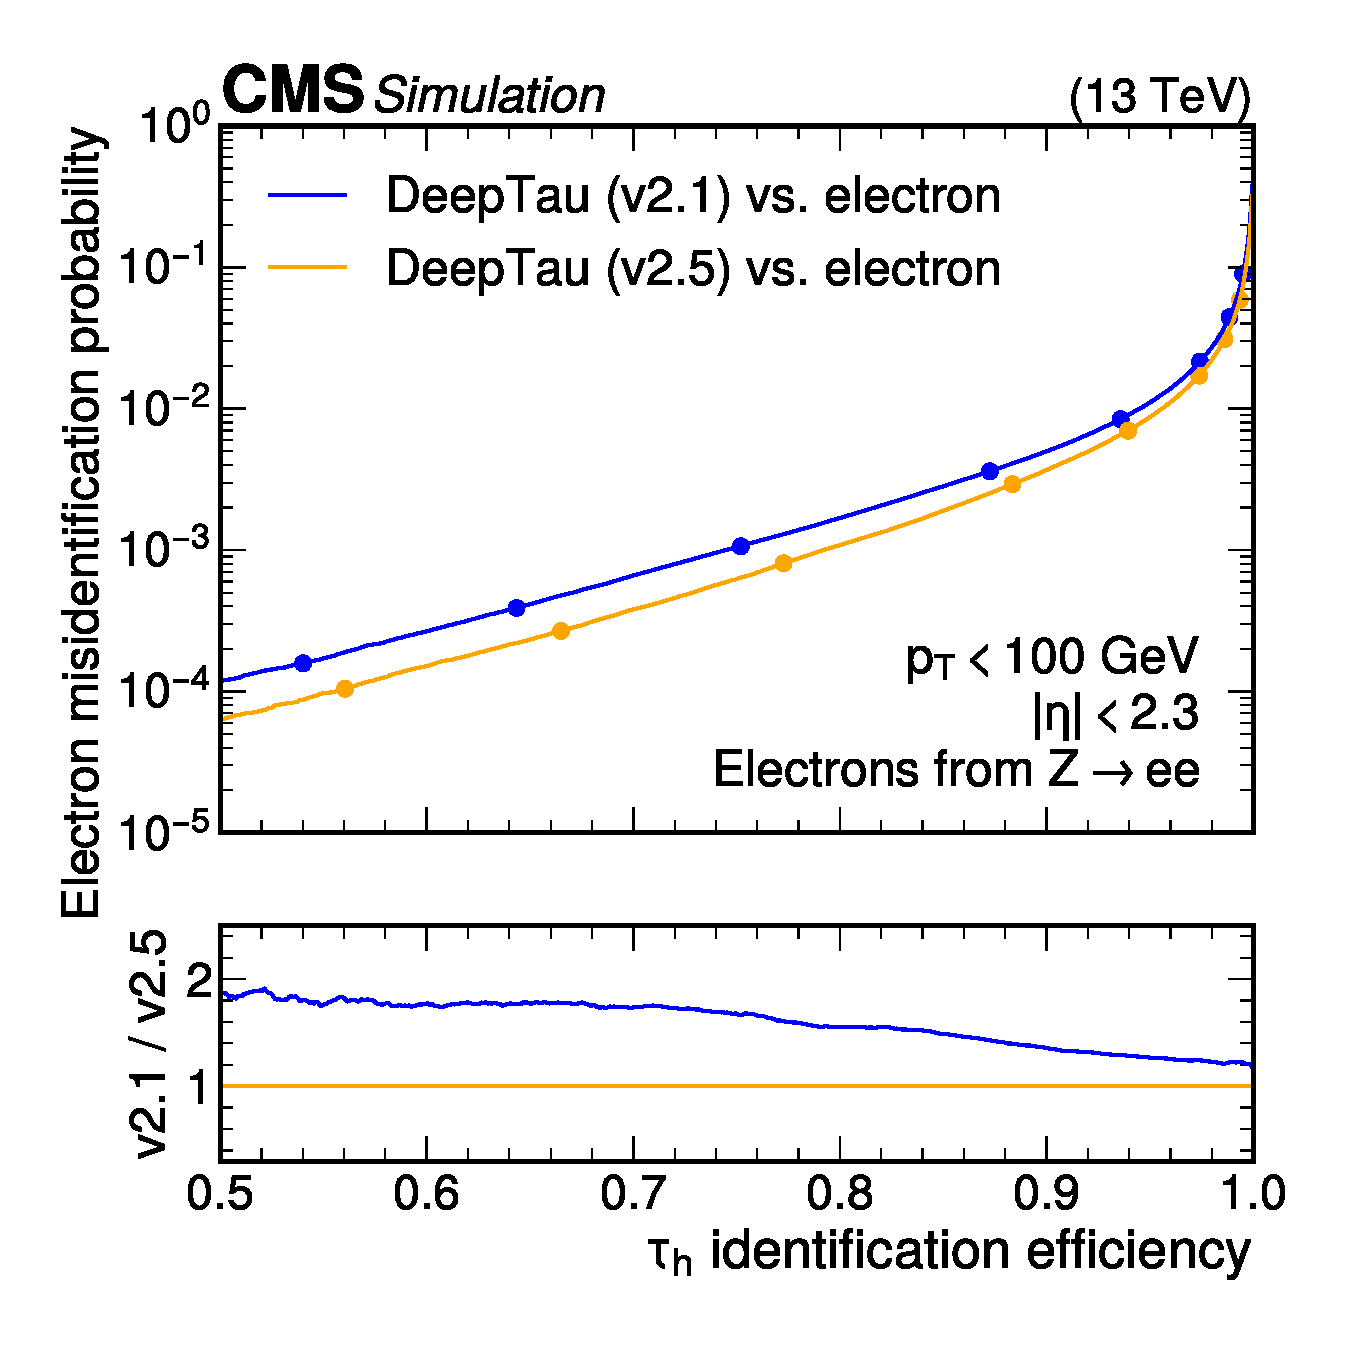
\includegraphics[width=\linewidth]{figures/chapter_III/CMS-TAU-24-001_Figure_007-a.pdf}
        \caption{\textsc{VSe}}
        \label{fig:DeepTau2p5VSe}
    \end{subfigure}
    \hfill
    \begin{subfigure}[t]{0.32\linewidth}
        \centering
        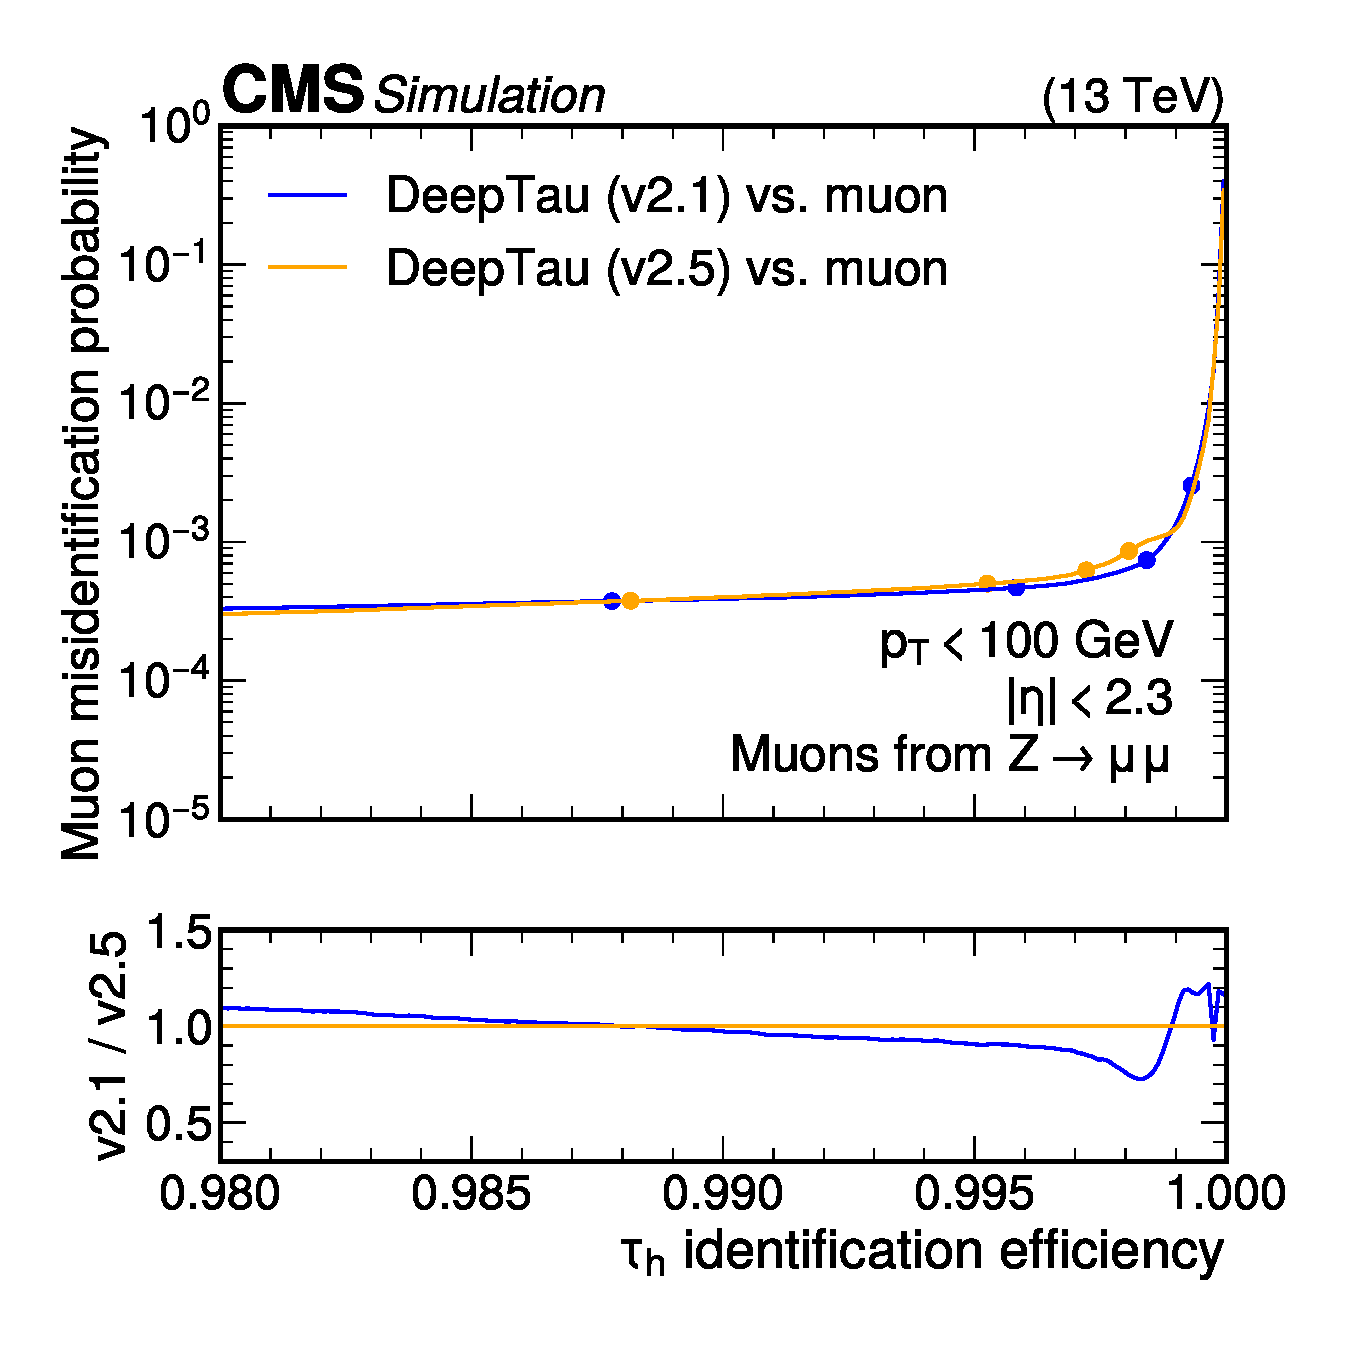
\includegraphics[width=\linewidth]{figures/chapter_III/CMS-TAU-24-001_Figure_008-a.pdf}
        \caption{\textsc{VSmu}}
        \label{fig:DeepTau2p5VSmu}
    \end{subfigure}
    \caption{Misidentification probability of quark and gluon jets (a), electrons (b) and muons (c) as a function of the identification efficiency for genuine $\tau_h$, for the \textsc{DeepTau} v2.1 (blue) and v2.5 (orange) discriminants. The efficiency is evaluated with $H\to\tau\tau$ events and the misidentification probabilities with $t\bar{t}$, $Z\to ee$ and $Z\to\mu\mu$ events, respectively, all simulated with 2018 conditions, for $\tau_h$ candidates with $p_T<100$ GeV and $|\eta|<2.3$. The working points are indicated by filled circles, and the lower panels show the ratio between both versions~\cite{CMS-TAU-24-001}.}
    \label{fig:DeepTau_versions}
\end{figure}

The second novelty of v2.5 is the use of domain adaptation~\cite{CMS-TAU-24-001}. Since v2.1 was trained only on simulation, any mismodeling of its inputs translated into differences between data and simulation in its output. To reduce them, v2.5 is trained on a mixture of simulated events and collision data, so that the network learns to classify $\tau_h$ candidates while avoiding the features that are described differently in data and in simulation. The classification itself is still learned only from simulation, while the collision data come from a sample of $Z\to\tau\tau\to\mu\tau_h$ events rich in genuine $\tau_h$ — the same final state used for the validation in Section \ref{sec:Tau_validation}. As a result, the agreement between data and simulation improves in the highest-score bins, and the corrections that analyses must apply move closer to unity.
%As a result, the agreement between data and simulation improves in the highest-score bins, where the difference in the last bin of the 2018 data used for the training is reduced from $17.4\%$ to $0.9\%$, and also in the 2022 data~\cite{CMS-TAU-24-001}, so that the corrections that analyses must apply move closer to unity.

%


%The corrections are systematically closer to unity for \textsc{v2.5} than for \textsc{v2.1} in both data-taking periods, which confirms the improvement in data-to-simulation agreement brought by the domain adaptation. Their absolute value remains below unity, an effect attributed to the modelling of hadronization and to imperfections in the simulation of the detector alignment and of the track hit reconstruction efficiency~\cite{CMS-TAU-24-001}. The agreement is visibly better for the 2018 dataset, which benefits from an optimized legacy reprocessing and from more mature algorithm calibrations than the early Run-3 data collected in 2022.



%In summary, the use and continuous development of deep-learning algorithms has proven essential for the challenging task of identifying $\tau_h$ leptons. These algorithms effectively complement the HPS reconstruction, yielding highly satisfactory results in background rejection. As a result, these developments significantly reduce the misidentification rate while preserving the efficiency for genuine $\tau_h$ leptons, thereby increasing the overall performance of $\tau$-based analysis.



\subsection{Alternative strategies for \texorpdfstring{$\tau_h$}{τh} identification}
\label{subsec:PNet}
%
In recent years, a different approach to $\tau_h$ identification has emerged in CMS as part of a \textit{unified jet tagging} strategy, in which the $\tau_h$ is treated as one more type of jet, and a single network classifies each jet according to its origin, whether a $b$ quark, a $c$ quark, a light quark, a gluon, an electron, a muon or a hadronically decaying $\tau$ lepton. This approach consistently models the correlations between the identification of the different objects, allows the selection to be optimized against specific sources of contamination, and concentrates computing resources in a single algorithm, used both in the offline reconstruction and in the HLT. Two algorithms follow this strategy, \textsc{ParticleNet} (\textsc{PNet})~\cite{PNet} and the Unified Particle Transformer (\textsc{UParT})~\cite{Qu:2022mxj,CMS-UParT}, both already introduced in Section \ref{subsec:Jets} for the identification of $b$ jets. 


\subsubsection{The Particle Net algorithm}
%
\textsc{PNet} represents the jet as a \textit{particle cloud}, an unordered set of its constituent PF candidates, in contrast with the image in the $\eta$-$\phi$ plane used by \textsc{DeepTau} and with the ordered lists of particles used by \textsc{DeepJet} (Section \ref{subsec:Jets}). This is a natural representation of a jet, whose constituents have no intrinsic order and are distributed irregularly in space. The particle cloud is processed by a graph neural network, a family of architectures suited to sets of elements without a fixed order or geometric structure, in which the features of each particle are updated using those of its nearest neighbors, so that the network learns the relations between the constituents. Unlike \textsc{DeepTau}, whose inputs rely on the intermediate reconstruction performed by HPS, \textsc{PNet} uses only the properties of the individual constituents of the jet, without any previous $\tau_h$-specific reconstruction.

At the time of its introduction, \textsc{PNet} achieved state-of-the-art performance in jet tagging, clearly surpassing the existing methods~\cite{PNet}, and it has since been widely adopted in CMS. Its main application in Run 3, however, has been the identification of $b$ and $c$ jets, for which it was the recommended algorithm in 2022 and 2023 (Section \ref{subsec:Jets}). For $\tau_h$, its use is so far limited to the HLT, where it replaced the online version of \textsc{DeepTau} in 2024 (Section \ref{sec:triggers}), while offline analyses, including the one presented in this thesis, still rely on \textsc{DeepTau}.




\subsubsection{The Unified Particle Transformer algorithm}
%
\textsc{UParT} also represents the jet as a particle cloud, but processes it with a transformer architecture, whose self-attention mechanism weighs the relation between every pair of constituents at once, instead of only between neighbors. Additionally, the \textsc{UParT} algorithm introduces variables that characterize the interaction between jet constituents and secondary vertices, known as pairwise interaction features, enhancing the sensitivity to internal structure of the jet

The first version of \textsc{UParT} was released in 2024~\cite{CMS-UParT}, and an updated version, v2, trained on a dataset twice as large and with a larger network, in 2025~\cite{CMS-DP-2025-081}. As shown in Figure \ref{fig:btag_evolution}, \textsc{UParT} improves on the performance of \textsc{PNet} in the identification of $b$ jets, and it has replaced it as the recommended algorithm for this task since 2024.\medskip



\noindent In both algorithms, the $\tau_h$ is treated as a one more type of jet, and the network returns the probability that the jet belongs to each of the classes considered in the training, which correspond to jets originating from $b$ quarks, $c$ quarks, light quarks and gluons, and to electrons, muons and $\tau_h$ reconstructed as jets, together with a regression of the jet energy~\cite{CMS-UParT}. Therefore, algthough both algorithms were originally designed and customized for AK4 jet classification, they both perform in an inclusive manner heavy flavor and hadronic $\tau$ identification combined with a flavor-aware jet energy and jet resolution regression~\cite{CMS-UParT}. The $\tau_h$ classes are further split according to the charge and the decay mode of the $\tau$ lepton, so that the decay mode of a candidate is not reconstructed from its constituents, as in HPS, but corresponds to the $\tau_h$ class with the highest probability — labeled with the convention of Equation \ref{eq:tau_DM} —, and its charge is obtained in the same way. Since these classes are defined from the generated decay, the networks can separate the h$^{\pm}\pi^0$ and h$^{\pm}\pi^0\pi^0$ modes, which HPS merges into a single decay mode (Section \ref{subsec:Taus}). The class probabilities are then combined into three discriminants against jets, electrons and muons, analogous to those of \textsc{DeepTau} and each with its own set of working points, while the energy regression provides the visible $p_T$ of the $\tau_h$. The whole description of the candidate thus comes from the network itself, without relying on any previous $\tau_h$-specific reconstruction.

Whether these techniques offer a performance competitive with or complementary to that of \textsc{DeepTau} cannot be inferred from their architectures alone, since each algorithm operates on a different reconstructed object, and is assessed in Section \ref{subsec:tau_IDcomparison}. The main features of the three algorithms are summarized in Table \ref{tab:algo_comparison}.
%
\begin{table}[h!]
    \centering\footnotesize
    \begin{tabular}{l l l l}
        \hline
         & \textbf{HPS+\textsc{DeepTau}} & \textbf{CHS+\textsc{PNet}} & \textbf{PUPPI+\textsc{UParT}} \\
        \hline
        Input object      & HPS $\tau_h$ candidate & AK4 jet & AK4 jet \\
        Inputs            & high- and low-level & low-level & low-level \\
        Representation    & $\eta$-$\phi$ grids & particle cloud & particle cloud \\
        Architecture      & CNN & graph NN & transformer \\
        Relations between & neighboring cells & nearest neighbors & all pairs, with \\
        constituents      &                   &                   & pairwise features \\
        Decay mode        & HPS (DMs $0$, $1$, $10$, $11$) & network (DMs $0$, $1$, $2$, $10$, $11$) & network (DMs $0$, $1$, $2$, $10$, $11$) \\
        Charge            & HPS & network & network \\
        Outputs           & \textsc{VSjet}, \textsc{VSe}, \textsc{VSmu} & jet flavor and $\tau_h$ classes, & jet flavor and $\tau_h$ classes, \\
                          &                                             & $p_T$ regression & $p_T$ regression \\
        \hline
    \end{tabular}
    \caption{Summary of the main features of the three $\tau_h$ identification algorithms compared in this chapter.}
    \label{tab:algo_comparison}
\end{table}




%Thus, as a particle-cloud tagger, the algorithm uses information directly from the PF candidates — which constitute the elements of the cloud — and is trained using low-level inputs and their correlations. Additionally, the \textsc{UParT} algorithm introduces variables that characterize the interaction between jet constituents and secondary vertices, known as pairwise interaction features, enhancing the sensitivity to internal jet structure. The transformer architecture provides greater flexibility for capturing global patterns, thereby complementing the description based on particle interactions characteristic of graph-based approaches such as~\textsc{PNet}.






\subsection{Comparison between \texorpdfstring{$\tau_h$}{τh} identification algorithms}
\label{subsec:tau_IDcomparison}
%DP2025-073 
To understand the complementarity of the described algorithms for identifying hadronic $\tau$ leptons based on advanced ML techniques, the subsequent section presents a comparison of the performance of each of them: \textsc{DeepTau v2.5}, \textsc{PNet} and \textsc{UParT v2}. The comparison will be made in terms of efficiency in the reconstruction and identification of genuine $\tau_h$ versus the ability to reject misidentified objects, as well as the accuracy in classifying $\tau$ decay modes, with the aim of discerning the strenghts of each algorithm and understanding how they complement one another. 

As previously discussed, a key distinction between the algorithms lies in the neural network architectures they exploit to perform the identification. However, this task requires the use of different reconstructed objects as input for each respective algorithm. To ensure a valid comparison, it is essential to consider the distinct reconstructed objects on which each algorithm operates. As indicated previously, \textsc{DeepTau} operates directly on HPS $\tau_h$ candidates; \textsc{PNet} and \textsc{UParT}, on the other hand, are fed AK4 jets that have been reconstructed by CMS taking into account the subtraction of pileup particles using dedicated algorithms, described in Section \ref{subsec:Jets}: charged-hadron substraction (CHS) and pileup-per-particle identification (PUPPI). Therefore, given the varying reconstruction efficiencies of these objects, a unified collection of $\tau$ candidates is defined, obtained as the union of HPS $\tau$ candidates, CHS jets, and PUPPI jets, to which a very loose selection is applied.

Accordingly, the performance of the classifiers is evaluated by taking into account the reconstruction efficiency of their associated reconstruction algorithm. This evaluation is based on ROC curves that show the fraction of no-$\tau_h$ objects that pass the discriminant (misidentification probability) compared to the fraction of genuine $\tau_h$ from the unified collection that pass the discriminant (efficiency) for each individual discriminant: \textsc{VSjet}, \textsc{VSe} and \textsc{VSmu}. This is depicted in Figure \ref{fig:ROC_tauID}, which demonstrates the performance of each discriminant for quark and gluon jets, electrons, and muons misidentified as $\tau_h$ using HPS+\textsc{DeepTau} (blue in the figure), CHS+\textsc{PNet} (yellow), PUPPI+\textsc{PNet} (red), and PUPPI+\textsc{UParT} (purple), where the solid markers indicate the respective working points. As illustrated in Figure \ref{fig:ROC_tauID}, the intrinsic efficiency of the HPS reconstruction is approximately \textcolor{red}{70\%}, and it can be easily recovered using \textsc{PNet}/\textsc{UParT}. The ROC curves also yield different conclusions depending on the discriminant evaluated. Thus, for discrimination agains quark and gluon jets, CHS+\textsc{PNet} demonstrates the most optimal global performance, with HPS+\textsc{DeepTau} offering a close second in the high-purity regime, configuration frequently employed in analyses; whereas in discrimination against electrons and muons, \textsc{UParT} emerges as the leader in performance, with HPS+\textsc{DeepTau} ranking second in the high-purity regime.

UParT achieves the best performance, followed by HPS+DeepTau in high-rejection mode, where its efficiency is not limited by the inefficiency of the HPS reconstruction.

The comparison must be read along two different axes. At a fixed efficiency within the
range accessible to all algorithms, the performances are comparable: CHS+\textsc{PNet}
provides the lowest jet misidentification rate, reducing it by 15--25\% with respect to
HPS+\textsc{DeepTau}, whereas PUPPI+\textsc{UParT} performs worse than
HPS+\textsc{DeepTau} against jets and clearly better against electrons and muons. The
qualitative difference appears instead in the accessible range: HPS+\textsc{DeepTau}
saturates at a $\tau_h$ efficiency of about 70\%, set by the HPS reconstruction itself,
while the jet-based taggers extend up to approximately 90\%, recovering candidates that HPS
does not reconstruct at all.


\begin{figure}[htbp]
    \centering
    
    \begin{subfigure}{0.32\textwidth}
        \centering
        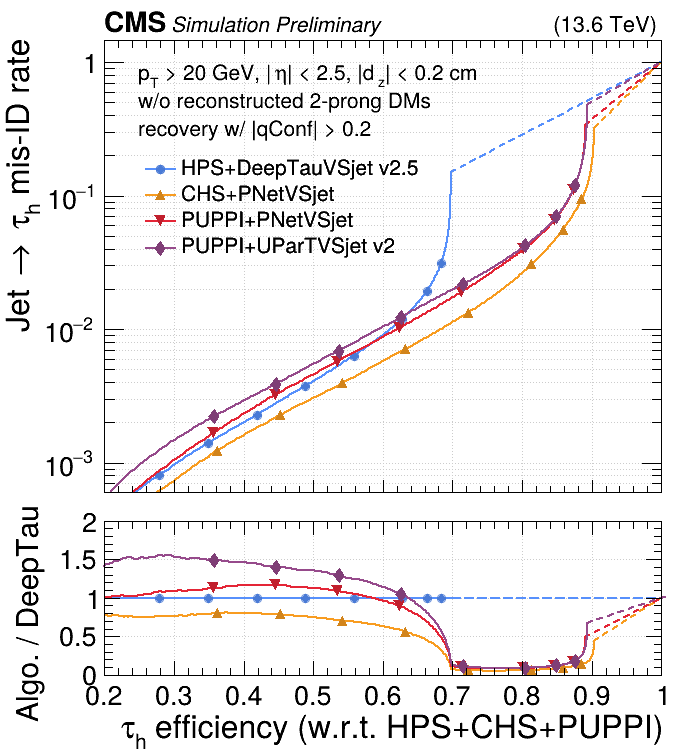
\includegraphics[width=\linewidth]{figures/chapter_III/ROC_IDvsJET.png}
        \caption{\textsc{VSjet}}
    \end{subfigure}
    \hfill
    \begin{subfigure}{0.32\textwidth}
        \centering
        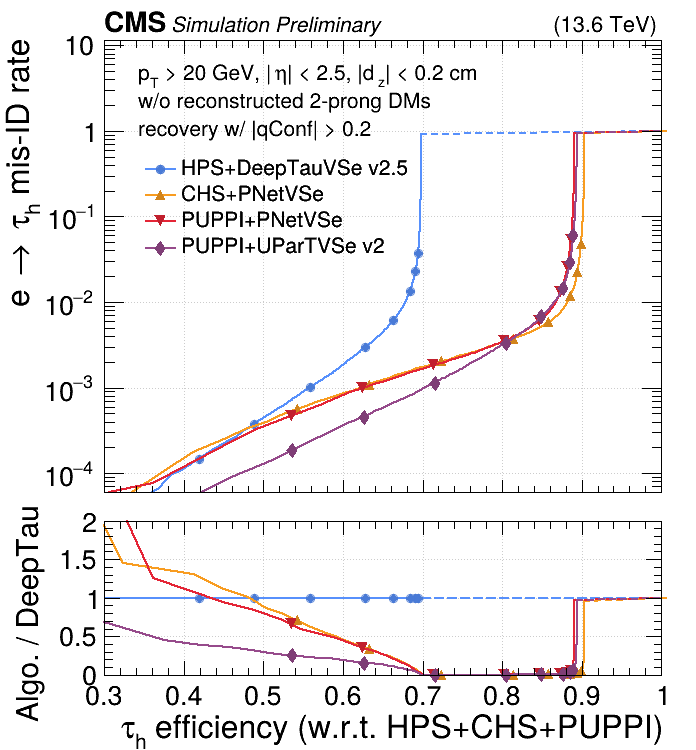
\includegraphics[width=\linewidth]{figures/chapter_III/ROC_IDvsE.png}
        \caption{\textsc{VSe}}
    \end{subfigure}
    \hfill
    \begin{subfigure}{0.32\textwidth}
        \centering
        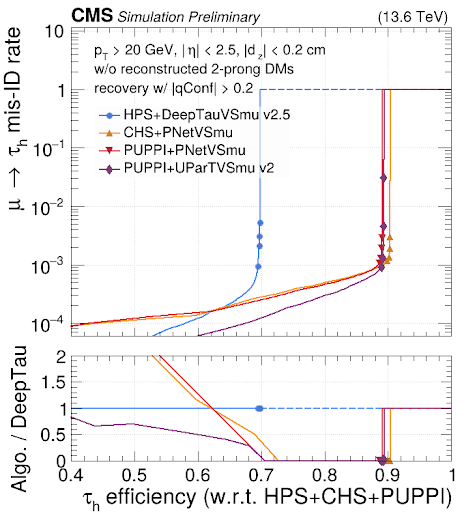
\includegraphics[width=\linewidth]{figures/chapter_III/ROC_IDvsMU.png}
        \caption{\textsc{VSmu}\textcolor{red}{ calidad de imagen}}
    \end{subfigure}
    
    \caption{ROC curves illustrating the performance of the \textsc{DeepTau}, \textsc{PNet}, and \textsc{UParT} algorithms to discriminate quark and gluon jets (a), electrons (b) and muons (c) misidentified as $\tau_h$ candidates. The efficiencies are evaluated taking into account the preceding reconstruction and pileup mitigation algorithms used, labeled HPS, CHS, and PUPPI. Extracted from \textcolor{red}{ref}}
    
    \label{fig:ROC_tauID}
\end{figure}

The key finding from this comparison is the competitive performance of these algorithms across various scenarios. Therefore, the subsequent concern to be adressed is the overlap between the $\tau_h$ candidates identified by each algorithm.

This is illustrated in Figure \ref{fig:venn_combined}, which displays the overlap and complement between $\tau_h$ candidates from the various reconstruction and identification combinations for the described algorithms. This behavior is represented graphically via Venn diagrams, which present the proportion
of candidates identified exclusively by each algorithm or concurrently by multiple algorithms following the application of the Medium WP of the discriminant \textsc{VSjet}. It has been determined that CHS+\textsc{PNet} and PUPPI+\textsc{UParT} can successfully recover between 24-32\% of genuine $\tau_h$ candidates that have not been reconstructed by the HPS algorithm or identified by \textsc{DeepTau}. However, it should be noted that these recovered candidates are more likely to be misidentified jets. This illustrates the complementary nature of the algorithms: while \textsc{DeepTau} maintains high purity, \textsc{PNet} and \textsc{UParT} demonstrate highly efficient performance capable of recovering lost candidates.


\begin{figure}[h!]
    \centering

    \begin{subfigure}[t]{0.48\linewidth}
        \centering
        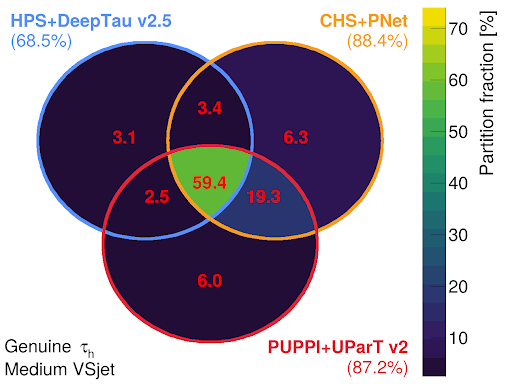
\includegraphics[width=\linewidth]{figures/chapter_III/Venn_1.png}
        \caption{Genuine $\tau_h$ candidates}
        \label{fig:venn1}
    \end{subfigure}
    \hfill
    \begin{subfigure}[t]{0.48\linewidth}
        \centering
        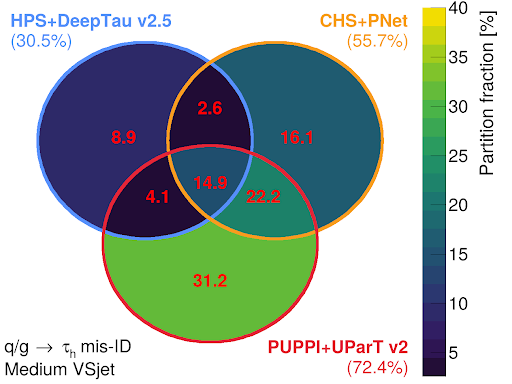
\includegraphics[width=\linewidth]{figures/chapter_III/Venn_2.png}
        \caption{Quark and gluon jets misidentified as $\tau_h$}
        \label{fig:venn2}
    \end{subfigure}

    \caption{Venn diagrams illustrating the overlap and complement between $\tau_h$ candidates from the HPS+\textsc{DeepTau} (blue circle), CHS+\textsc{PNet} (orange circle) and PUPPI+\textsc{UParT} (red circle) algorithms for genuine $\tau_h$ candidates (a) and jets misidentified (b). The red number and fill color of each partition indicate the fraction of candidates it contains relative to the union of all partitions in the diagram. Extracted from \textcolor{red}{ref}}
    \label{fig:venn_combined}
\end{figure}

\textsc{PNet} and \textsc{UParT} have been shown to outperform in terms of $\tau_h$ recovery. Additionally, in terms of decay mode assignment, they both exhibit superior capability compared to the HPS algorithm, as they provide finer resolution in the separation of decay modes and distinguish between the $h^{\pm}\pi^0$ and $h^{\pm}\pi^0\pi^0$ DMs, which were merged by HPS.\medskip


Overall, the revised comparison indicates that the performance of the algorithms varies across misidentified objects and in their description of the internal structure of the $\tau_h$ candidate. Each of the classifiers has been found to have different strengths. \textsc{PNet} provides the best rejection of misidentified quark and gluon jets, while \textsc{DeepTau v2.5} and \textsc{UParT v2} provide the best rejection of misidentified electrons and muons. When it comes to assign the DM, \textsc{PNet} and \textsc{UParT v2} show overall superiority. This underscores the potential value of exploring diverse machine learning architectures in enhancing $\tau_h$ candidate identification, and the efficacy of combining these architectures to achieve the most advanced $\tau_h$ identification to date.

% Finally, it should be noted that while this text has focused on standard CMS strategies, additional algorithms have been developed to target topologies not adequately covered by standard reconstruction and identification techniques. These additional algorithms are briefly mentioned below: \textsc{DisTau} \textcolor{red}{ref}, used to identify $\tau_h$ candidates that have been produced displaced from the primary interaction vertex; \textsc{Boosted DeepTau} \textcolor{red}{ref}, specially designed for $\tau_h$ candidates that have been produced as part of a boosted $\tau\tau$ system; and a modified version of HPS algorithm tailored to low-$p_T$ $\tau_h$ candidates \textcolor{red}{ref}, accompanied by a dedicated energy flow neural network called \textsc{TauNet} \textcolor{red}{ref}. \cite{CMS-DP-2025-047}

\section{Performance with \texorpdfstring{$\sqrt{13.6}$}{√13.6} TeV data}
\label{sec:Tau_validation}

Validating the performance of the algorithms presented for reconstructing and identifying $\tau_h$ in real data is an essential step in ensuring the reliability of any physics analysis using hadronic $\tau$ particles. Therefore, although the algorithms detailed in the previous section have been extensively optimized and evaluated in simulations, it is imperative to verify their performance in each data run conducted by CMS, and, by doing so, monitor the behavior of the techniques developed and actually used in analyses under real experimental conditions.

As part of this thesis work, the $\tau_h$ reconstruction and identification performance of these algorithms has been systematically validated within the Tau POG by evaluating data from all years of Run-3, covering the data-taking periods from 2022 through early 2026. The following sections present two fundamental aspects of this validation. First, Section \ref{subsec:Data-MC-agreement} presents the results in terms of Data to MC comparison for all the aforementioned data-taking periods, which resulted in an internal CMS Detector Performance note \textcolor{red}{DP-2025-074}. Second, Section \ref{subsec:TES_checks} addresses the stability and consistency of performance across the different years of data collection and, consequently, across the changing conditions of the detector. \textcolor{red}{invertir el orden? hablar primero de stability de los datos y luego data-to-MC?}


\subsection{Data-to-MC comparison in Run-3}
\label{subsec:Data-MC-agreement}

To evaluate the performance of the $\tau_h$ modeling in CMS, the simulation is compared with data collected during different data-taking periods for various distributions of relevant variables. The simulation utilized for the comparison is based on the Summer24 NanoAODv15 campaign, which serves as the most up-to-date reference, incorporating the variables required for the recent \textsc{PNet} and \textsc{UParT v2} models. The Monte Carlo (MC) simulation is validated using data from all years of Run-3 processed (or reprocessed in the case of data collected during 2022 and 2023) within the same NanoAODv15 campaign, ensuring consistency between the comparison. 

The simulated samples include the main processes contributing to the selected final state: Drell-Yan, top quark pair production, W+jets, and di-Boson processes. The simulation is partially calibrated to describe the data, including corrections unrelated to the $\tau$ particles, such as calibration of the number of pileup interactions, corrections to the $t\bar{t}$ system momentum and $Z$ boson transverse momentum spectra, and correction factors for muon identification and isolation efficiency. Multijet QCD contribution, which is challenging to model in simulation, is estimated directly from the data in a sideband region adjacent to that used in the validation, and is extrapolated to the signal region.

%\textcolor{red}{No dar tanto detalle?}
%To ensure the accuracy of the validation, events in both data and MC simulations are selected within a well-controlled region enriched in $Z\rightarrow \tau\tau \rightarrow \mu \tau_h$ events using a combination of triggers to select muons with $p_T>24$ GeV. A series of selection criteria is the applied to the $\mu$ and $\tau$ candidates, as briefly described in the following. First, both candidates must have opposite electric charges to ensure that the selected topology is compatible with the $Z\rightarrow \tau\tau$ decay and to suppress other background contributions. The $\mu$ is selected using standard CMS cuts: $p_T>26$ GeV, $|\eta|<2.4$, isolation $<0.15$, and the Medium Working Point for the Muon ID in CMS \textcolor{red}{ref}. The $\tau$ is selected with $p_T > 20$ GeV and $|\eta|<2.5$, and it satisfies the following Working Points corresponding to \textsc{DeepTau v2.5}: VVLoose \textsc{VSe}, Tight \textsc{VSmu}, and Medium \textsc{VSjet}, corresponding to reconstruction efficiencies of 99\%, 99.5\% y 70\% respectively. This selection is replaced by an analogous one for the \textsc{PNet} and \textsc{UParT v2} algorithms. Finally, to define the enriched region in $Z\rightarrow \tau\tau \rightarrow \mu \tau_h$, a cut is made on the transverse mass in the muon - Missing Transverse Energy (MET) system, $m_T(\mu,MET)$, requiring $m_T(\mu,MET)<65$ GeV, as illustrated in Figure \ref{fig:mT_cut_baseline}. This is motivated to exclude

To guarantee the precision of the validation, events in both data and MC simulations are selected within a well-controlled region enriched in $Z\rightarrow \tau\tau \rightarrow \mu \tau_h$ events using data collected with muon triggers. A series of standard selection criteria is applied to the $\mu$ and $\tau$ candidates, which will not be detailed, to ensure a well-reconstructed set of objects. To facilitate reliable identification performance, the $\tau_h$ must satisfy the following Working Points (WPs) in accordance with \textsc{DeepTau v2.5}: VVLoose \textsc{VSe}, Tight \textsc{VSmu}, and Medium \textsc{VSjet}, corresponding to reconstruction efficiencies of 99\%, 99.5\% y 70\% respectively. This selection is replaced by an analogous one for the \textsc{PNet} and \textsc{UParT v2} algorithms, aiming at keeping the same yield for the $Z\rightarrow \tau\tau \rightarrow \mu \tau_h$ process. To define the region enriched in $Z\rightarrow \tau\tau \rightarrow \mu \tau_h$, a requirement is imposed on the transverse mass in the muon - $p_T^\text{miss}$ system, $m_T(\mu, p_T^\text{miss})$, requiring $m_T(\mu,MET)<65$ GeV, as illustrated in Figure \ref{fig:mT_cut_baseline}. This cut excludes the high-$m_T$ region dominated by W+jet contribution, where the $\mu$ originates from a $W\rightarrow\mu\nu$ decay and the accompanying jet has a high probability of being misidentified as a $\tau_h$. In contrast, genuine $Z\rightarrow\tau\tau$ events populate the low-$m_T$ region due to the softer and less back-to-back MET arising from the $\tau$ decays, making this selection highly effective for isolating the signal enriched region.

% \begin{figure}
%     \centering
%     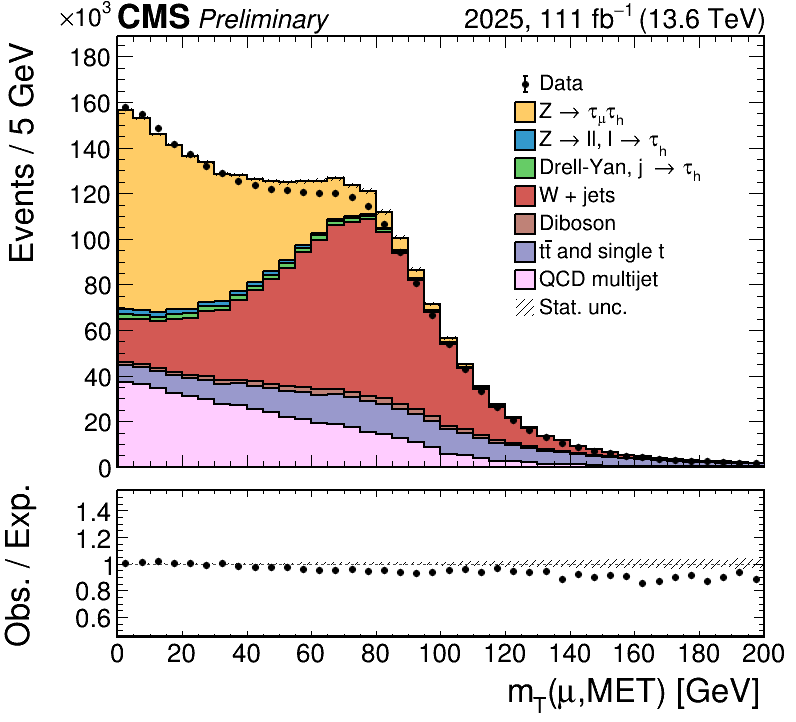
\includegraphics[width=1\linewidth]{figures//chapter_III/mT_2025.png}
%     \caption{Enter Caption}
%     \label{fig:mT_cut_baseline}
% \end{figure}
\begin{figure}
    \centering
    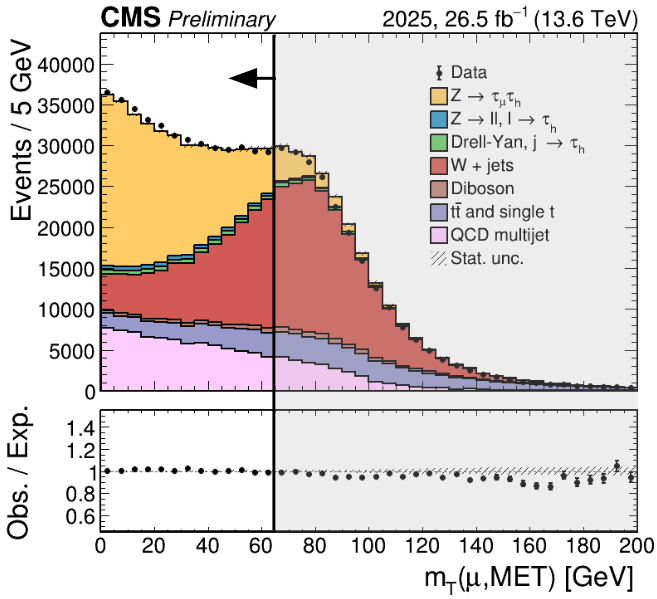
\includegraphics[width=0.5\linewidth]{figures//chapter_III/mT_2025_captura.png}
    \caption{Transverse mass distribution in the $\mu$-MET system, comparing 2025 data with MC simulation. The black line delimits the $Z\rightarrow\tau\tau\rightarrow\mu\tau_h$ enriched signal region below $m_T<65$ GeV, as marked by the arrow. The shaded region indicates the excluded region rich in W+jets contribution, and therefore with a high jet misidentification rate. \textcolor{red}{Hacerla en buena calidad (es screenshot)}}
    \label{fig:mT_cut_baseline}
\end{figure}

Figure \ref{fig:kinematics_mu_tau_2024} shows the simulation-to-data agreement in the signal region, as previously defined, for the kinematic behavior of the reconstructed objects, namely the $\mu$ and the $\tau_h$. To illustrate the validity of the modeling of the reconstructed objects, the distributions in $p_T$, $\eta$ and $\phi$ for both $\mu$ and $\tau_h$ are displayed for a representative year, 2025 in this case. The figure indicate that there are no substantial discrepancies in the shape of the distributions, and the data-to-MC agreement is generally as expected. Minor normalization discrepancies resulting from the absence of dedicated corrections are also anticipated.


\begin{figure}[htbp]
    \centering

    %------------------ ROW 1: MUON ------------------%
    \begin{subfigure}[t]{0.32\linewidth}
        \centering
        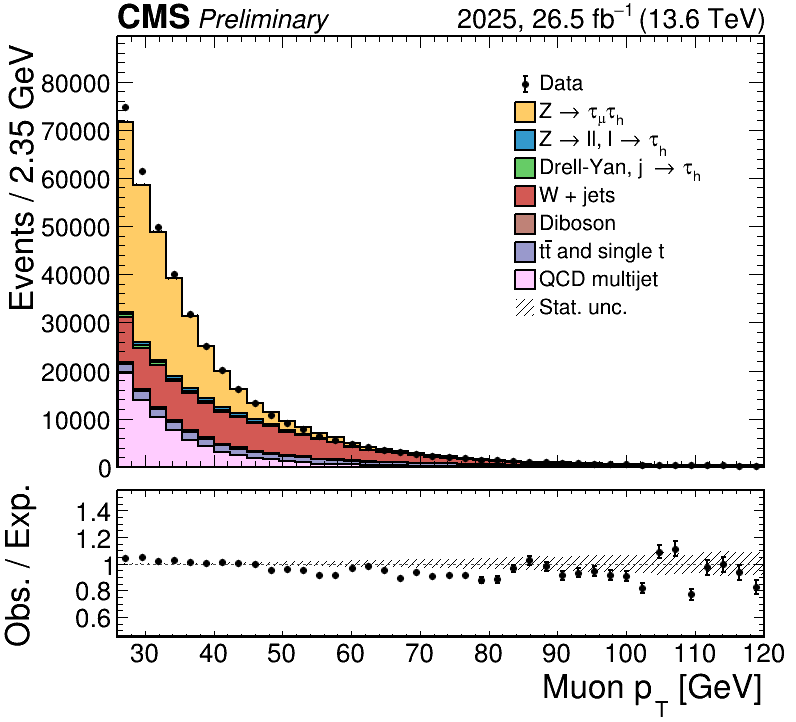
\includegraphics[width=\linewidth]{figures/chapter_III/muon_pt_2025.png}
        \caption{$p_T(\mu)$}
        \label{fig:muon_pt_2024}
    \end{subfigure}
    \hfill
    \begin{subfigure}[t]{0.32\linewidth}
        \centering
        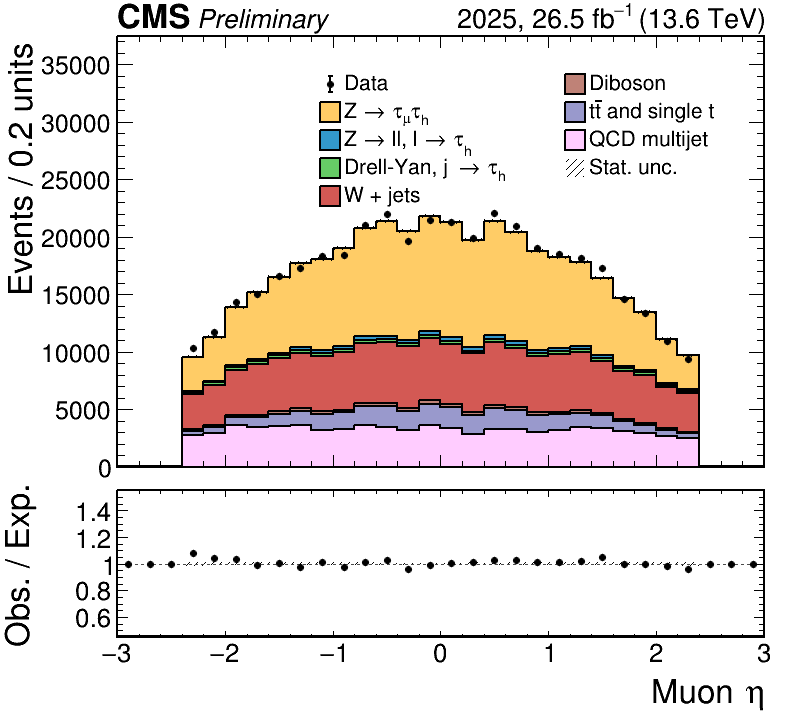
\includegraphics[width=\linewidth]{figures/chapter_III/muon_eta_2025.png}
        \caption{$\eta(\mu)$}
        \label{fig:muon_eta_2024}
    \end{subfigure}
    \hfill
    \begin{subfigure}[t]{0.32\linewidth}
        \centering
        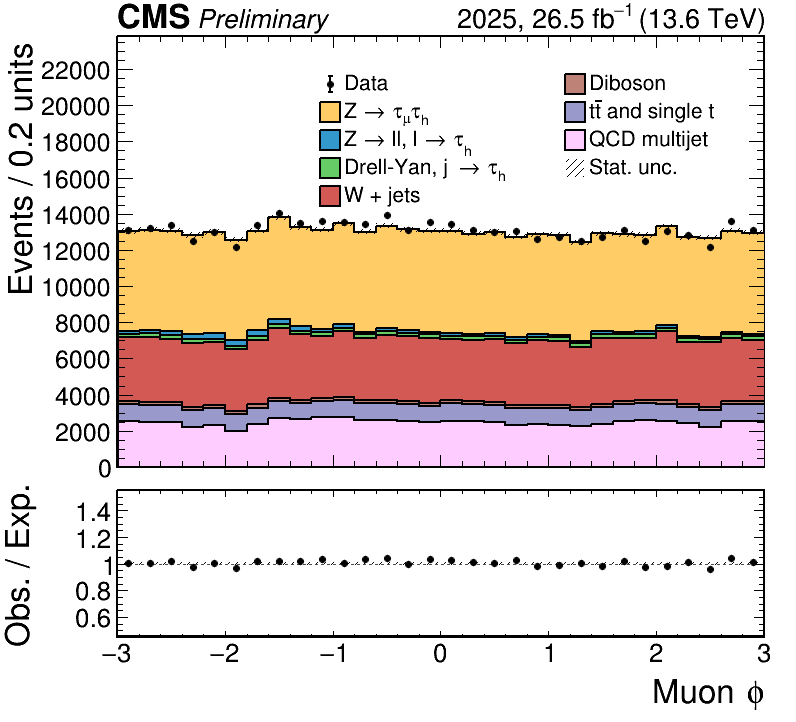
\includegraphics[width=\linewidth]{figures/chapter_III/muon_phi_2025.png}
        \caption{$\phi(\mu)$}
        \label{fig:muon_phi_2024}
    \end{subfigure}

    \vspace{0.5cm}

    %------------------ ROW 2: TAU ------------------%
    \begin{subfigure}[t]{0.32\linewidth}
        \centering
        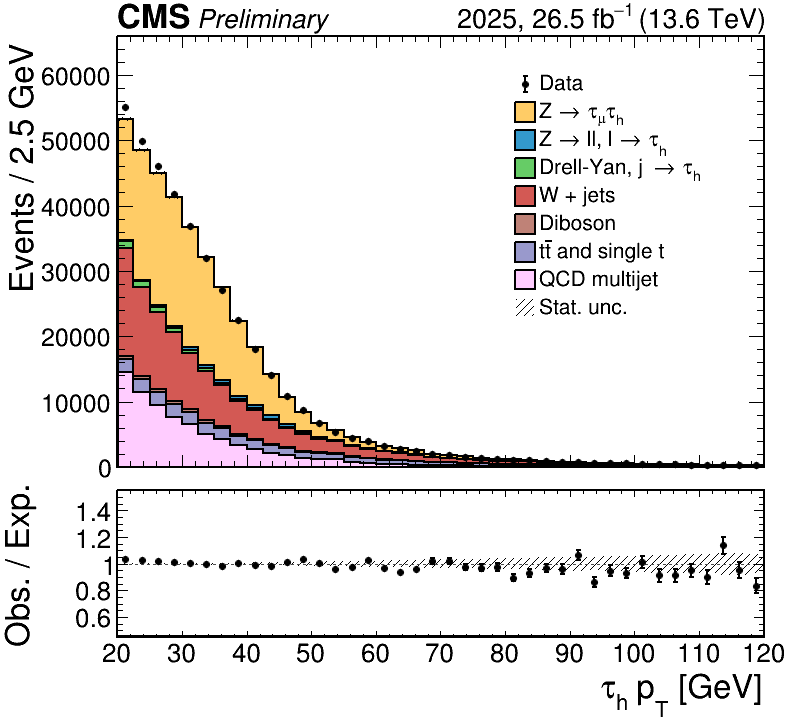
\includegraphics[width=\linewidth]{figures/chapter_III/tau_pt_2025.png}
        \caption{$p_T(\tau_h)$}
        \label{fig:tau_pt_2024}
    \end{subfigure}
    \hfill
    \begin{subfigure}[t]{0.32\linewidth}
        \centering
        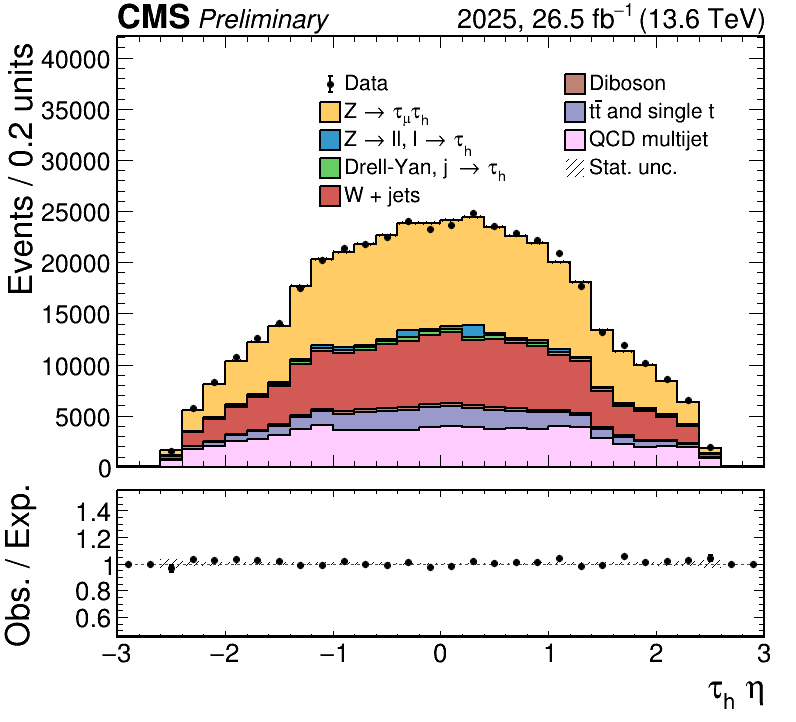
\includegraphics[width=\linewidth]{figures/chapter_III/tau_eta_2025.png}
        \caption{$\eta(\tau_h)$}
        \label{fig:tau_eta_2024}
    \end{subfigure}
    \hfill
    \begin{subfigure}[t]{0.32\linewidth}
        \centering
        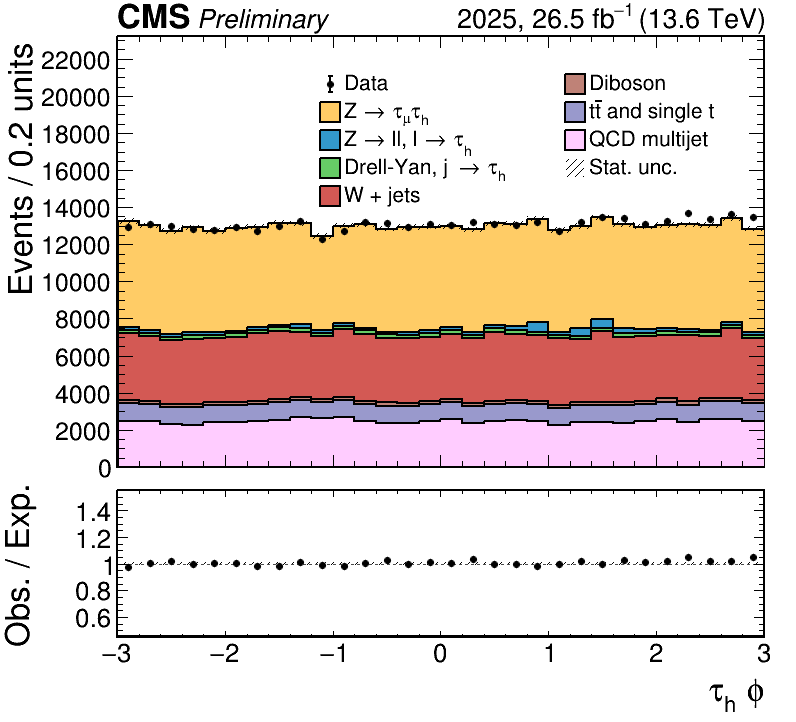
\includegraphics[width=\linewidth]{figures/chapter_III/tau_phi_2025.png}
        \caption{$\phi(\tau_h)$}
        \label{fig:tau_phi_2024}
    \end{subfigure}

    \caption{Comparison between data and simulation for the kinematic distributions of the muon (top row) and the $\tau_h$ candidate (bottom row) in the signal region using 2025 data}
    \label{fig:kinematics_mu_tau_2024}
\end{figure}

The reliability of the $\tau_h$ modeling across the various years of Run-3 is illustrated in Figure \ref{fig:mvis_all_years}. The reference variable used for comparison is the invariant mass of the visible objects in the $\mu\tau_h$ system, $m_{vis}$, since it is a robust observable that is sensitive to possible discrepancies in the $\tau_h$ reconstruction owing to the fact that the behavior of the $\mu$ is widely understood in CMS. The $m_{vis}$ distribution is shown separately for each of the data-taking periods, covering 2022, 2023, 2024, 2025, and 2026. All distributions demonstrate strong data/MC alignment, where the consistency of the shape over the years confirms the good performance in the reconstruction and identification of the $\tau_h$ during Run-3. However, for a more detailed overview, the subsequent Section \ref{subsec:TES_checks} thoroughly examines the stability in the performance of the data collected across the years in terms of relative efficiencies and misidentification rates.
%
%No $\tau_h$-related corrections are applied in these distributions: neither the identification efficiency scale factors nor the energy scale corrections discussed in Section \ref{...}. The residual normalization differences observed in the ratio panels are therefore a direct measure of the size of those corrections, rather than an indication of mismodelling of the $\tau_h$ reconstruction itself.
%
\begin{figure}[htbp]
    \centering

    %------------------ ROW 1 ------------------%
    \begin{subfigure}[t]{0.32\linewidth}
        \centering
        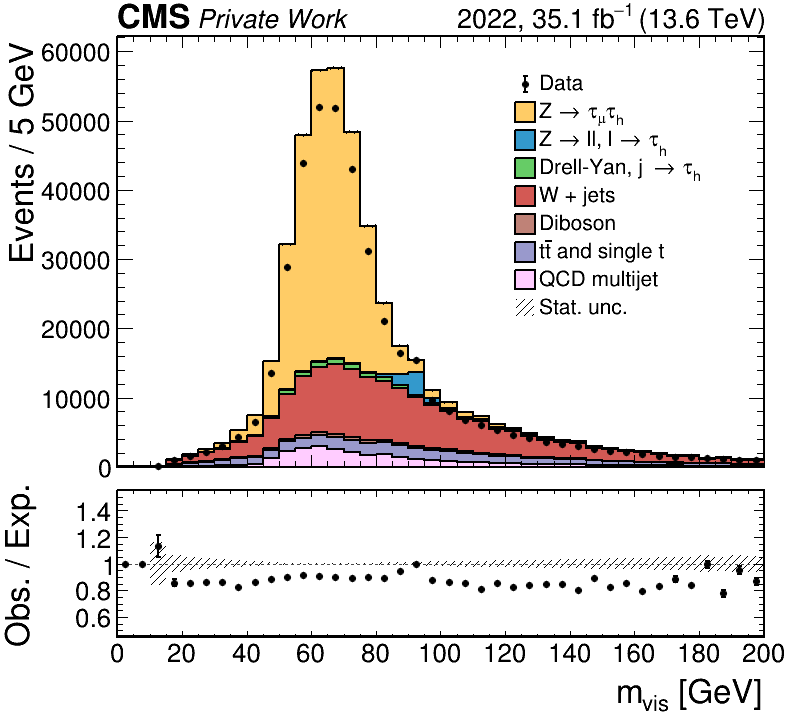
\includegraphics[width=\linewidth]{figures/chapter_III/mvis_2022.png}
        \caption{2022}
        \label{fig:mvis_2022}
    \end{subfigure}
    \hfill
    \begin{subfigure}[t]{0.32\linewidth}
        \centering
        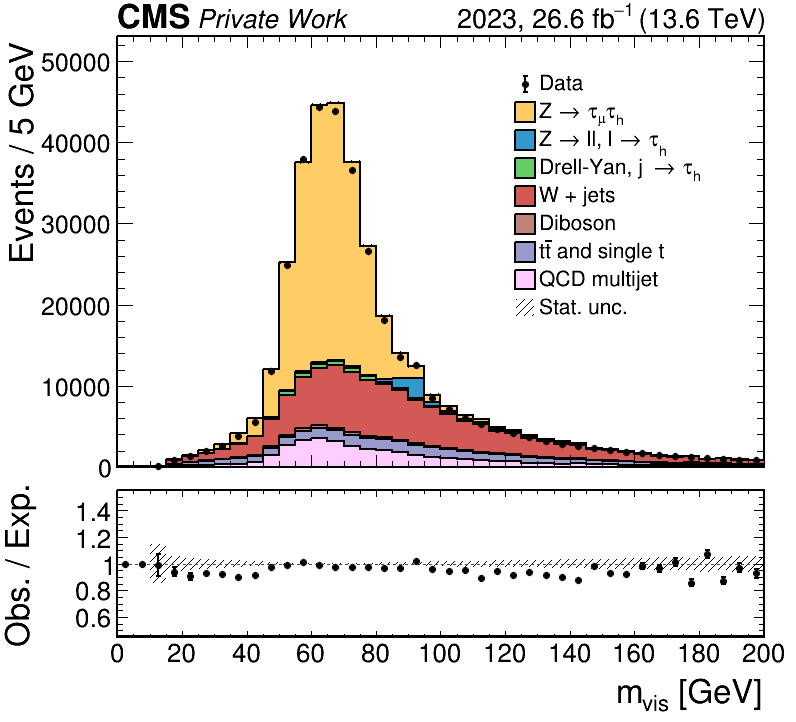
\includegraphics[width=\linewidth]{figures/chapter_III/mvis_2023.png}
        \caption{2023}
        \label{fig:mvis_2023}
    \end{subfigure}
    \hfill
    \begin{subfigure}[t]{0.32\linewidth}
        \centering
        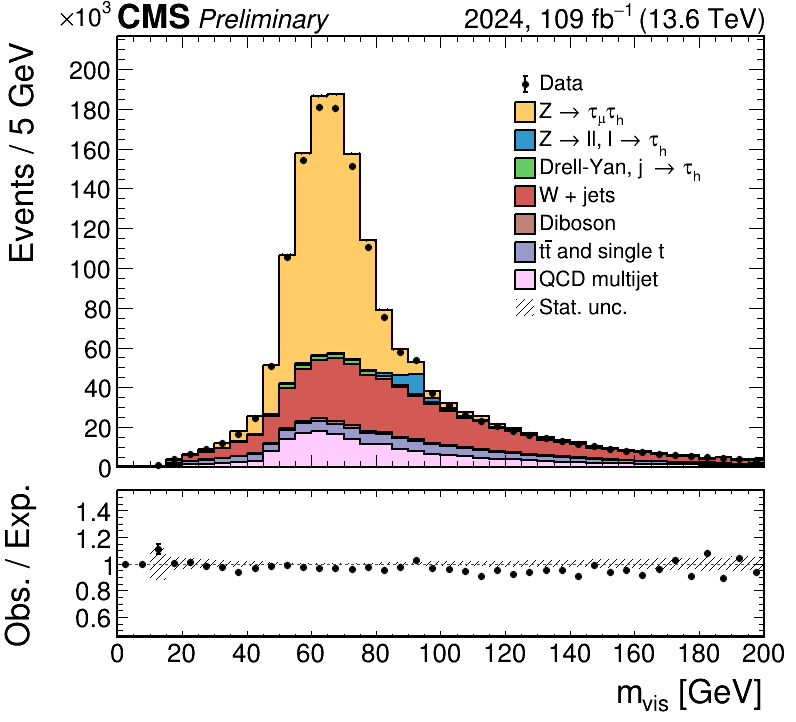
\includegraphics[width=\linewidth]{figures/chapter_III/mvis_DeepTau_2024.png}
        \caption{2024}
        \label{fig:mvis_2024}
    \end{subfigure}

    \vspace{0.6cm}

    %------------------ ROW 2 ------------------%
    \begin{subfigure}[t]{0.32\linewidth}
        \centering
        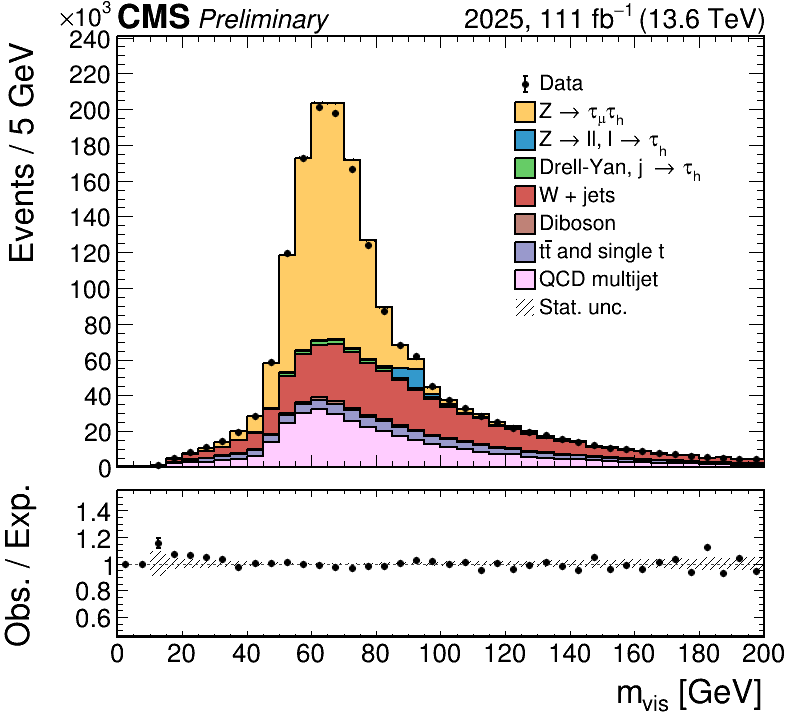
\includegraphics[width=\linewidth]{figures/chapter_III/mvis_DeepTau_2025.png}
        \caption{2025}
        \label{fig:mvis_2025}
    \end{subfigure}
    \hspace{0.03\linewidth} 
    \begin{subfigure}[t]{0.32\linewidth}
        \centering
        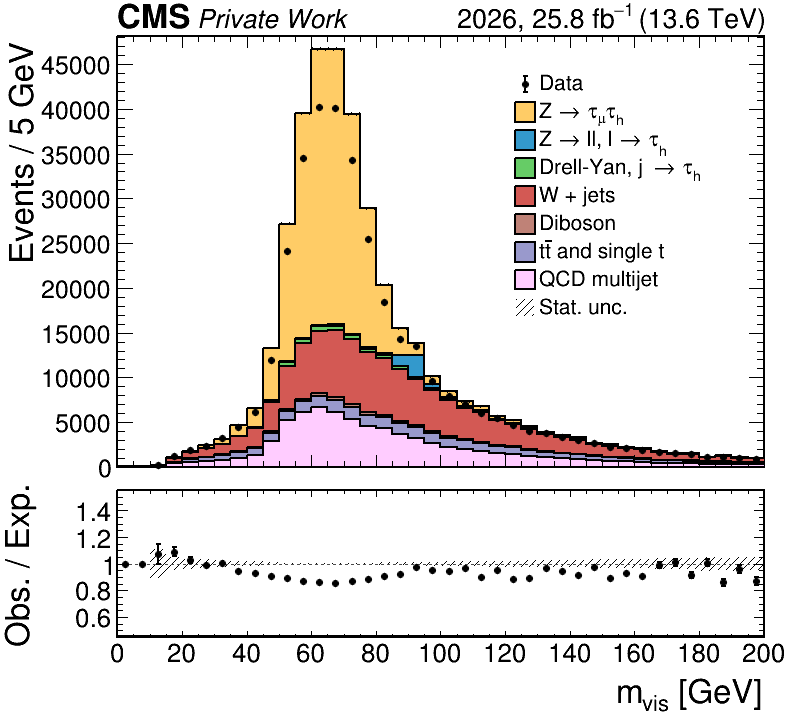
\includegraphics[width=\linewidth]{figures/chapter_III/mvis_2026.png}
        \caption{2026}
        \label{fig:mvis_2026}
    \end{subfigure}

    \caption{Comparison between data and simulation for the visible mass distribution $m_{vis}$ in the signal region for the years 2022 (a), 2023 (b), 2024 (c), 2025 (d) and 2026 (e).}
    \label{fig:mvis_all_years}
\end{figure}


The performance of the aforementioned $\tau_h$ identification algorithms (\textsc{DeepTau v2.5}, \textsc{PNet} and \textsc{UParT}) is compared in Figure \ref{fig:algorithms}, with data from 2024 serving as a reference. The figure illustrates the performance of each classifier through various sets of distribution:

\paragraph{Score distributions:}
The top row of Figure \ref{fig:algorithms} displays the score distributions of the discriminator \textsc{VSjet} returned by each identification algorithm, where the requirement that the $\tau_h$ candidates satisfy the medium \textsc{VSjet} WP has been removed. The range selected for each discriminator score distribution is chosen to ensure the retention of 90\% of the genuine hadronic $\tau$ candidates. The shape of the score distribution for each classifier shows discrepancies linked to the nature of each different architecture. The figure illustrates that the three $\tau_h$ identification algorithms demonstrate strong performance in terms of data-MC agreement, with \textsc{DeepTau} notably outperforming the others due to its domain adaptation feature.
% Since domain adaptation is currently implemented only in \textsc{DeepTau}, the larger data-to-simulation discrepancies observed for \textsc{PNet} and \textsc{UParT} would translate into larger correction factors and associated systematic uncertainties for any analysis adopting them.

\paragraph{Visible mass:}
The middle row serves as an example of the behavior of the visible mass $m_{vis}$ of the system reconstructed using different $\tau_h$ identification algorithms, demonstrating satisfactory simulation-to-data consistency in all cases. As outlined in Section \ref{subsec:tau_IDcomparison}, Figure \ref{fig:algorithms} illustrates how the three identification methods have distinct rejection levels for quark and gluon jets, electrons, and muons, resulting in different yields for each contributing process. Figure \ref{fig:venn_combined} showed the overlap between the algorithms in this regard. Therefore, the combination of two or more of these identification strategies can serve to optimize the selection of genuine $\tau_h$ candidates and the rejection of misidentified objects. This is demonstrated in Figure \ref{fig:mvis_PNetDeepTau_comb}, which shows the visible mass distribution obtained from the combined selection of \textsc{DeepTau v2.5} and \textsc{PNet} algorithms, providing the strongest rejection of misidentified $\tau_h$ candidates.

\paragraph{Decay mode assignment:}
Finally, the set of plots in the last row is intended to illustrate the differences in the assignment of decay modes performed by each algorithm. In these distributions, the $Z\to\mu\tau_h$ signal simulation is separated into its various decay modes to facilitate the visualization of the correct assignment of each decay mode per algorithm under study.

\begin{figure}[htbp]
    \centering

    %------------------ ROW 1: SCORES ------------------%
    \begin{subfigure}[t]{0.32\linewidth}
        \centering
        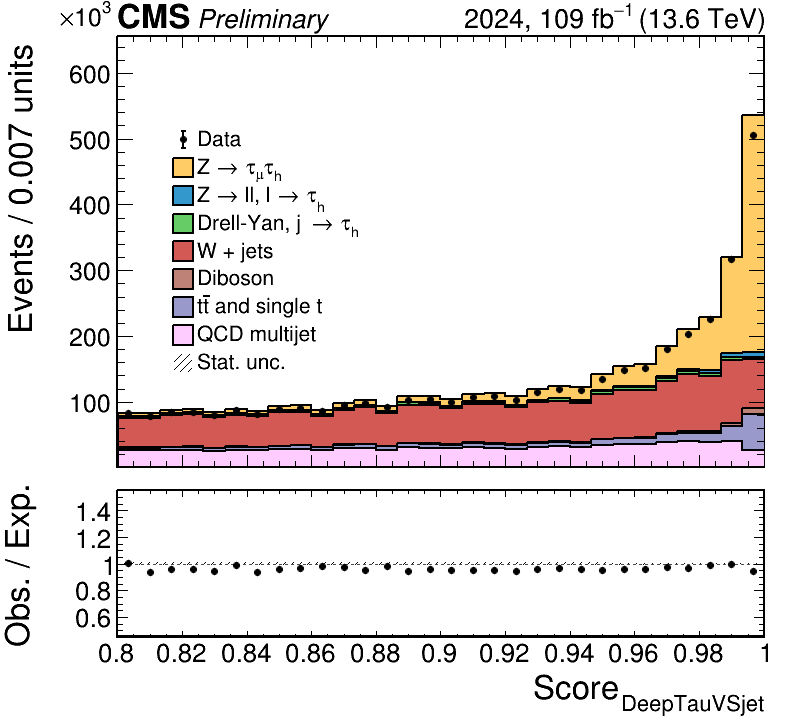
\includegraphics[width=\linewidth]{figures/chapter_III/score_DeepTau_vsJET_2024.png}
        \caption{\textsc{DeepTau v2.5} VSjet score}
        \label{fig:score_deeptau}
    \end{subfigure}
    \hfill
    \begin{subfigure}[t]{0.32\linewidth}
        \centering
        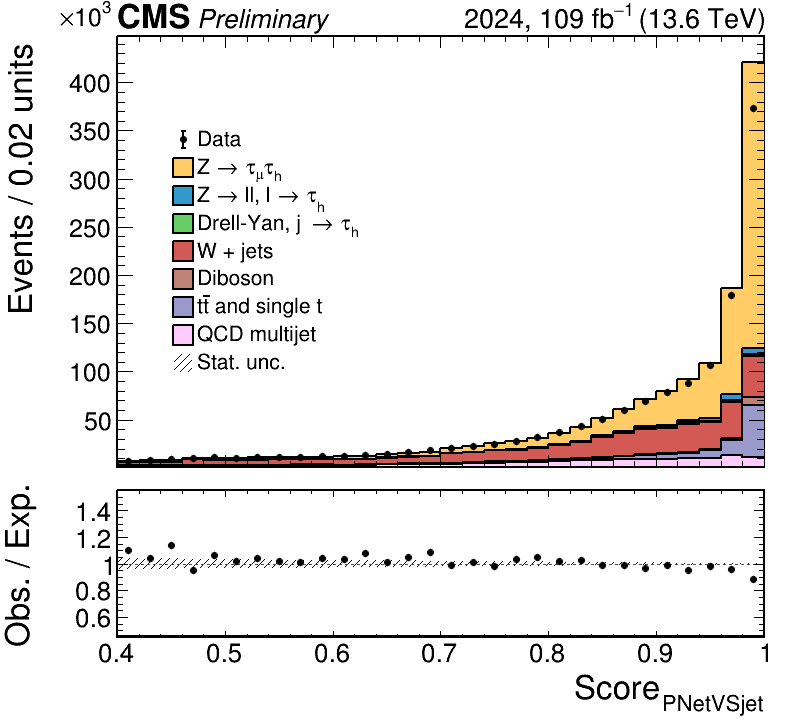
\includegraphics[width=\linewidth]{figures/chapter_III/score_PNet_vsJET_2024.png}
        \caption{\textsc{PNet} VSjet score}
        \label{fig:score_pnet}
    \end{subfigure}
    \hfill
    \begin{subfigure}[t]{0.32\linewidth}
        \centering
        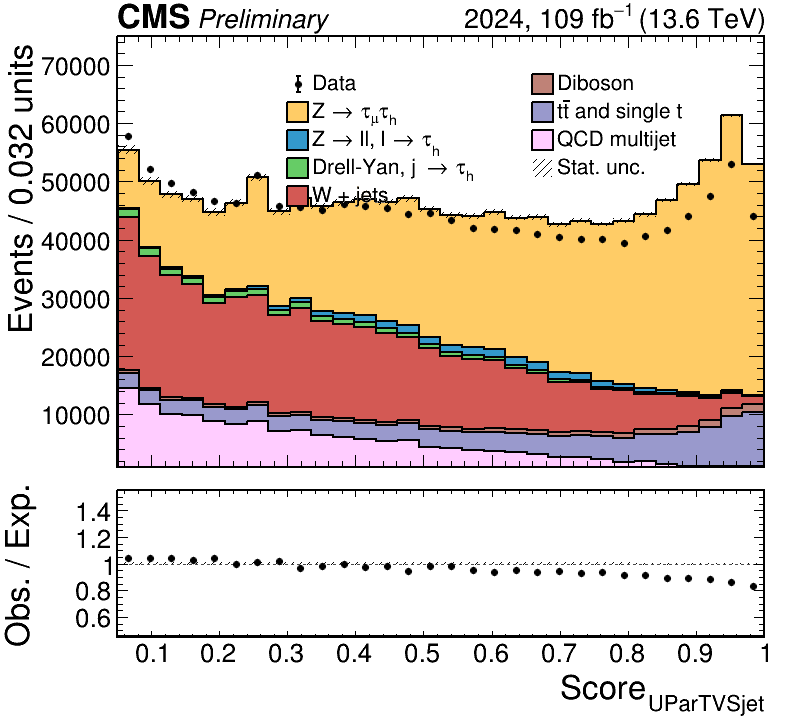
\includegraphics[width=\linewidth]{figures/chapter_III/score_UParT_vsJET_2024.png}
        \caption{\textsc{UParT v2} VSjet score}
        \label{fig:score_upart}
    \end{subfigure}

    \vspace{0.6cm}

    %------------------ ROW 2: MVIS ------------------%
    \begin{subfigure}[t]{0.32\linewidth}
        \centering
        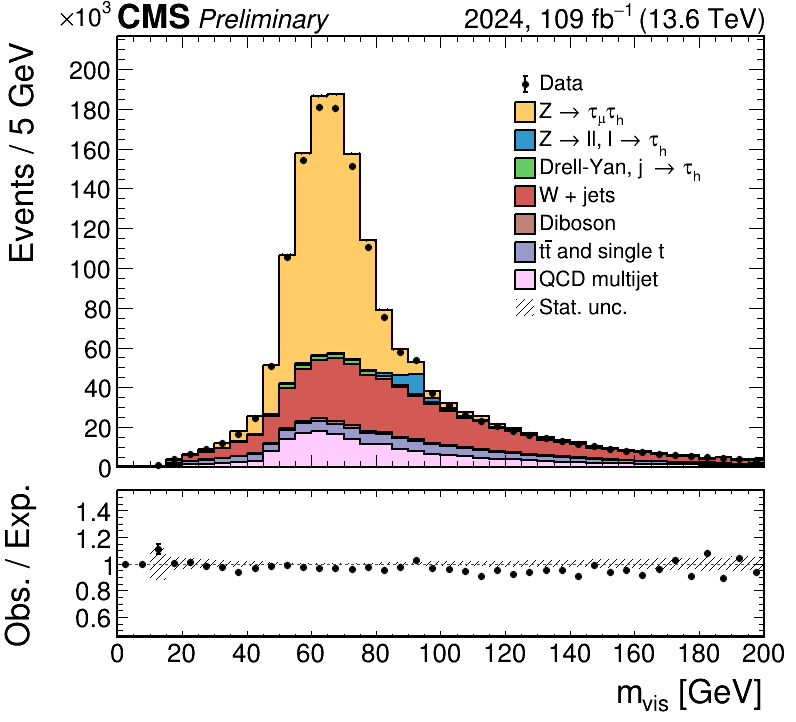
\includegraphics[width=\linewidth]{figures/chapter_III/mvis_DeepTau_2024.png}
        \caption{$m_{\mathrm{vis}}$ (\textsc{DeepTau v2.5})}
        \label{fig:mvis_deeptau}
    \end{subfigure}
    \hfill
    \begin{subfigure}[t]{0.32\linewidth}
        \centering
        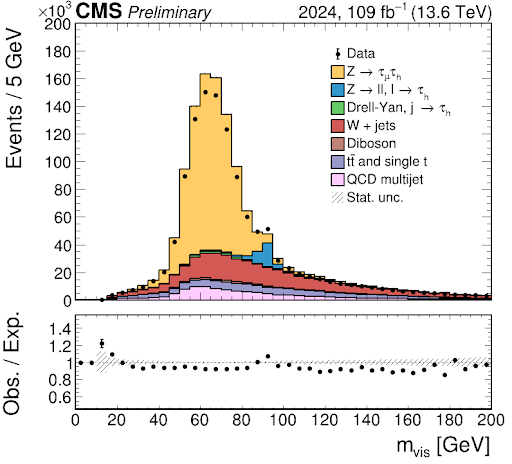
\includegraphics[width=\linewidth]{figures/chapter_III/mvis_PNet_2024.png}
        \caption{$m_{\mathrm{vis}}$ (\textsc{PNet})\textcolor{red}{coger en buena calidad}}
        \label{fig:mvis_pnet}
    \end{subfigure}
    \hfill
    \begin{subfigure}[t]{0.32\linewidth}
        \centering
        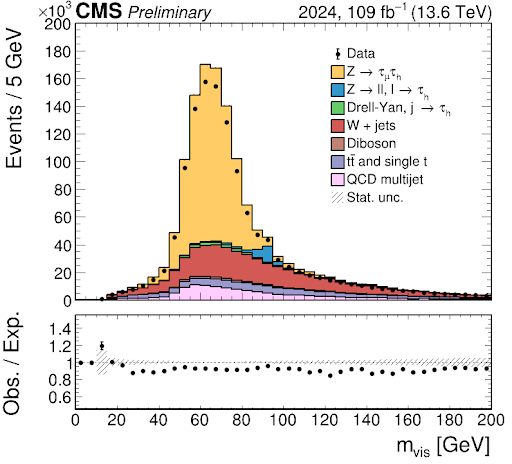
\includegraphics[width=\linewidth]{figures/chapter_III/mvis_UParT_2024.png}
        \caption{$m_{\mathrm{vis}}$ (\textsc{UParT v2})\textcolor{red}{coger en buena calidad}}
        \label{fig:mvis_upart}
    \end{subfigure}

    \vspace{0.6cm}

    %------------------ ROW 3: DECAY MODES ------------------%
    \begin{subfigure}[t]{0.32\linewidth}
        \centering
        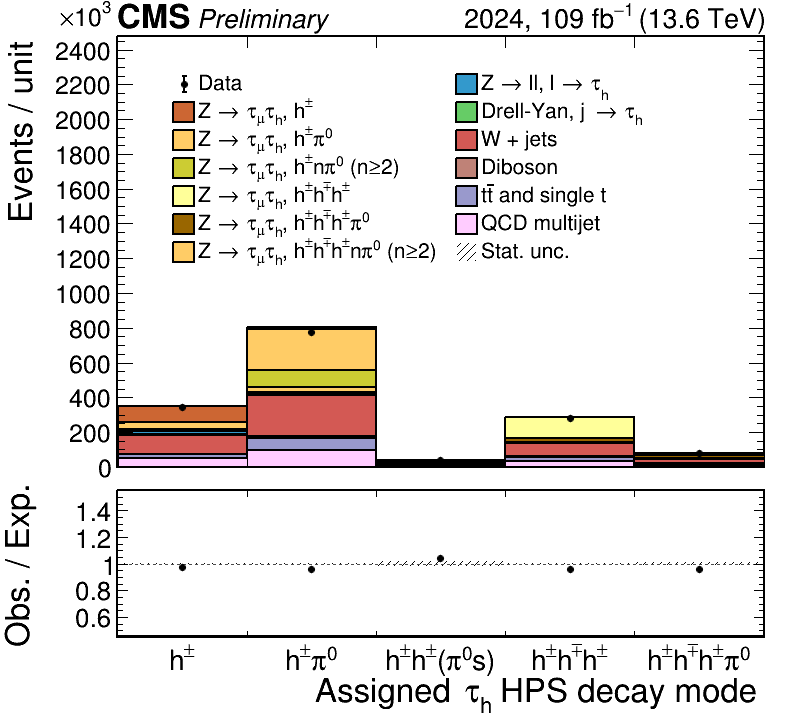
\includegraphics[width=\linewidth]{figures/chapter_III/HPS_DM_2024.png}
        \caption{Decay Mode (HPS)}
        \label{fig:dm_hps}
    \end{subfigure}
    \hfill
    \begin{subfigure}[t]{0.32\linewidth}
        \centering
        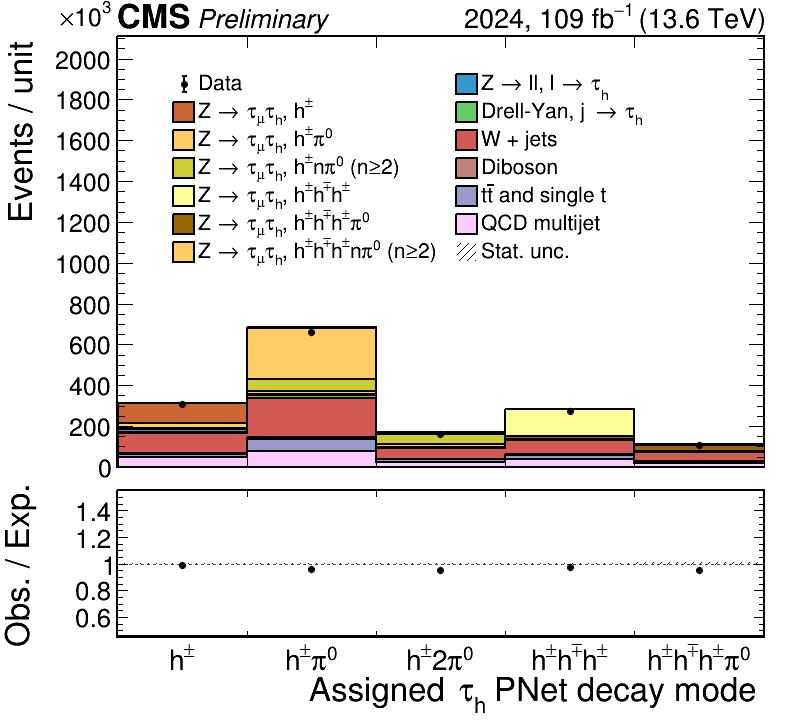
\includegraphics[width=\linewidth]{figures/chapter_III/PNet_DM_2024.png}
        \caption{Decay Mode (\textsc{PNet})}
        \label{fig:dm_pnet}
    \end{subfigure}
    \hfill
    \begin{subfigure}[t]{0.32\linewidth}
        \centering
        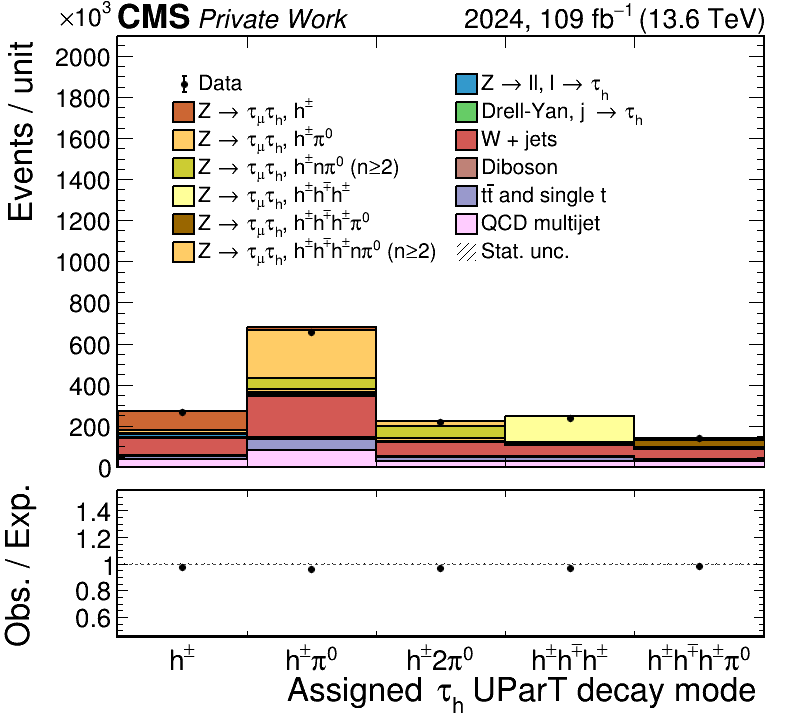
\includegraphics[width=\linewidth]{figures/chapter_III/UParT_DM_2024.png}
        \caption{Decay Mode (\textsc{UParT v2}) \textcolor{red}{REHACER}}
        \label{fig:dm_upart}
    \end{subfigure}

    \caption{
        Summary of the validation of the three $\tau_h$ identification algorithms with 2024 data. 
        \textbf{Top row:} score distributions of the \textsc{VSjet} discriminant for \textsc{DeepTau v2.5}, \textsc{PNet}, and \textsc{UParT v2}. 
        \textbf{Middle row:} visible mass distributions reconstructed with each algorithm. 
        \textbf{Bottom row:} decay mode assigned by each algorithm. 
    }
    \label{fig:algorithms}
\end{figure}

\begin{figure}
    \centering
    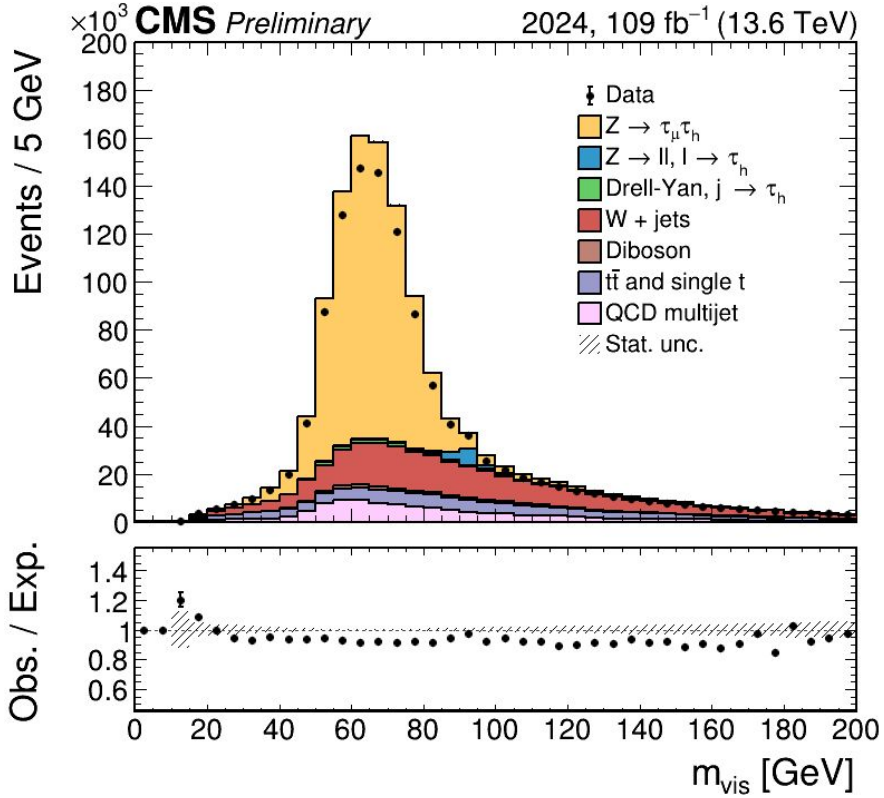
\includegraphics[width=0.6\linewidth]{figures//chapter_III/mvis_DeepTau&PNet.png}
    \caption{Visible mass distribution obtained from the combined selection of \textsc{DeepTau v2.5} and \textsc{PNet}, illustrating the enhanced rejection of misidentified $\tau_h$ candidates achieved when both algorithms are used simultaneously. \textcolor{red}{Es un screenshot, cogerlo en buena calidad}}
    \label{fig:mvis_PNetDeepTau_comb}
\end{figure}

These plots illustrate the difference in classifier response, mass reconstruction, and decay mode assignment across the three identification strategies, and thereby validate the performance of each algorithm in simulation relative to actual data.

\noindent Overall, the evaluation of $\tau_h$ modeling in terms of data-to-MC comparisons has confirmed the robustness of hadronic $\tau$ identification and reconstruction algorithms. To further validate the $\tau$ lepton behavior in CMS, the following section presents the consistency of data collection throughout Run-3, with the aim of addressing possible effects arising from evolving detector conditions.


\subsection{Stability of \texorpdfstring{$\tau_h$}{τh} performance in Run-3 data}
\label{subsec:TES_checks}
%presentación PPD (1): https://indico.cern.ch/event/1569864/contributions/6612866/attachments/3109869/5512492/TauPOG_2024_2025Data_PPD_2407.pdf
%presentación PPD (2): https://docs.google.com/presentation/d/178-DORdl0GOepSjdjDzxOgDB1sgRS6_t_pinHd4K7ro/edit?slide=id.g3c670cd6792_0_1#slide=id.g3c670cd6792_0_1

The previous section presented the Data-to-MC validation, which was designed to verify the correct modeling of $\tau_h$ reconstruction and identification in simulation. This section, in contrast, focuses on evaluating the actual response of the detector throughout the various periods of Run-3. Across these periods, the detector is subject to variations in its operating conditions due to increases in instantaneous luminosity and the aging of the components, which can influence key aspects of $\tau_h$ performance, such as the energy scale, identification efficiency and misidentification rate. Therefore, studying the stability of the collected data becomes imperative to ensure a reliable description of the data through Monte Carlo simulation. These studies thus serve as an independent verification process that complements simulation-based validation. 

The behavior of the data over the years is now addressed using an approach similar to the one presented in previous section. Events from the $Z\to\tau\tau\to\mu\tau_h$ process are selected using data collected with muon triggers and under a preselection criteria analogous to that in Section \ref{subsec:Data-MC-agreement}, with the exception that the $\tau$ must satisfy Tight \textsc{VSjet} WP criterion in order to maximize the purity in genuine $\tau_h$. This is done to ensure that consistency studies actually confirm that any variations across data-taking periods reflect genuine detector effects rather than changes in the background composition. For the studies outlined here, the \textsc{DeepTau} algorithm will be the sole discriminant employed. Furthermore, the cut on the transverse mass $m_T(\mu,MET) < 65$ GeV, as defined in Figure \ref{fig:mT_cut_baseline}, is maintained to preserve a region rich in genuine $\tau_h$ particles.

Figure \ref{figr:data_across_years} shows a comparison of the visible mass of the system $m_{vis}$ over the different periods of Run-3, from 2022 to 2026. Generally, a stable trend is observed across the different data-taking years, with a slight shift observed starting from 2024 onward \textcolor{red}{????}. While deviations of this nature are consistent with the impact of deteriorating detector conditions, they warrant a more detailed investigation of the stability of the data.

\begin{figure}
    \centering
    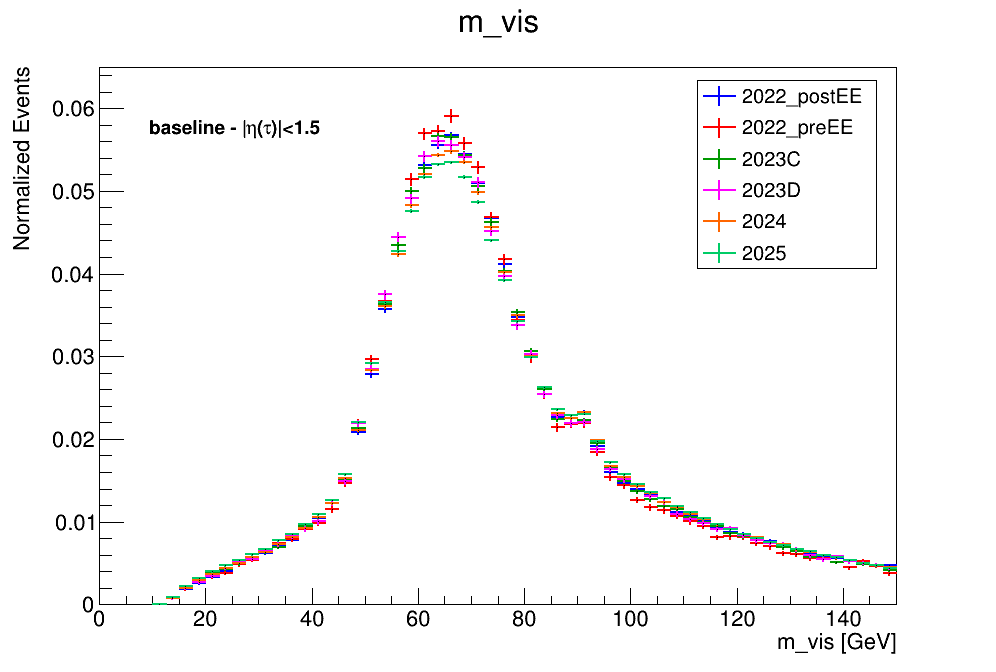
\includegraphics[width=0.5\linewidth]{figures//chapter_III/data_across_years_barrel.png}
    \caption{\textcolor{red}{rehacer el plot para todo eta, añadiendo full 25 + 26 y mejorando el estilo}}
    \label{fig:data_across_years}
\end{figure}

To provide a more detailed characterization of these effects, the visible mass of the $\mu\tau_h$ system in the region enriched with Drell-Yan events is studied. As illustrated in \ref{fig:ratio_plots}, this in-depth study provides valuable insights. The strategy employed consists of plotting the ratio of the $m_{vis}$ distribution across different years for a common reference period that varies for each panel, as explained in more detail in the figure caption. This approach serves to illuminate the distinctions between the various data sets. As a result, different behaviors can be observed:
\begin{itemize}
    \item The $m_{vis}$ region between $40 < m_{vis} < 90$ GeV corresponds to the $Z\to\tau\tau\to\mu\tau_h$ peak and is therefore dominated by genuine hadronic $\tau$ events. This region exhibits consistent behavior over the years, following a flat ratio in all cases, with a minor decline in efficiency towards the end of Run-3, indicating stability in the response of the detector to genuine $\tau_h$.
    \item Outside the $Z\to\tau\tau\to\mu\tau_h$ peak, in the tails of the $m_{vis}$ spectrum, the distribution is dominated by fake $\tau$ particles, primary from jets misidentified as $\tau_h$ in the W+jets background contribution. In these regions, a slight increase in events is observed for 2024, which becomes particularly noticeable in 2025 and 2026, highlighting the greater sensitivty to fakes.
\end{itemize}



%\begin{figure}
%    \centering
%    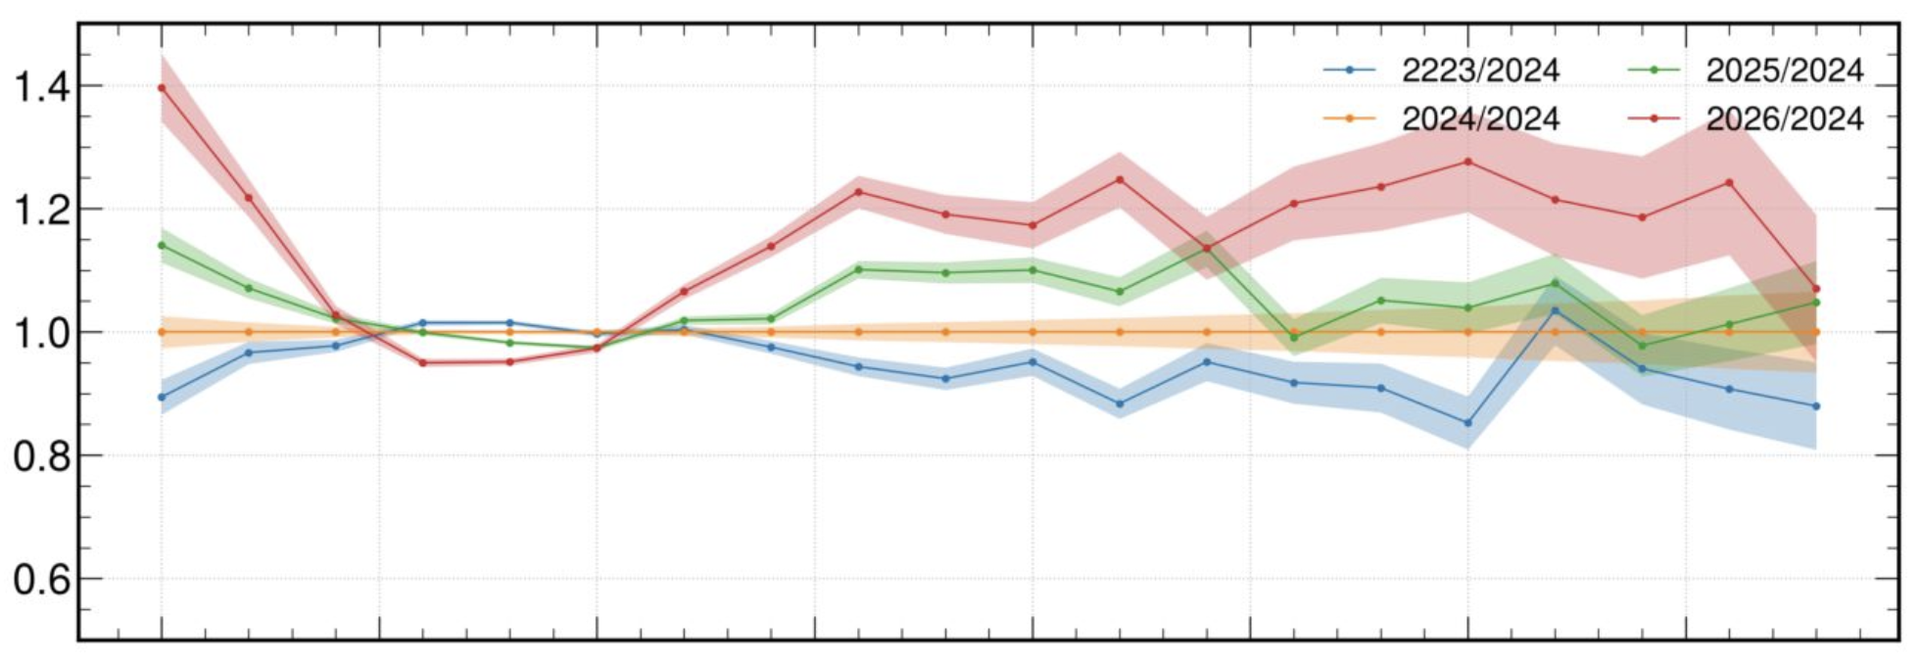
\includegraphics[width=0.5\linewidth]{figures//chapter_III/mvis_ratio_fulldata.png}
%    \caption{\textcolor{red}{estaría bien los plots anteriores pero con todos los años}}
%    \label{fig:placeholder}
%\end{figure}

\begin{figure}
    \centering
    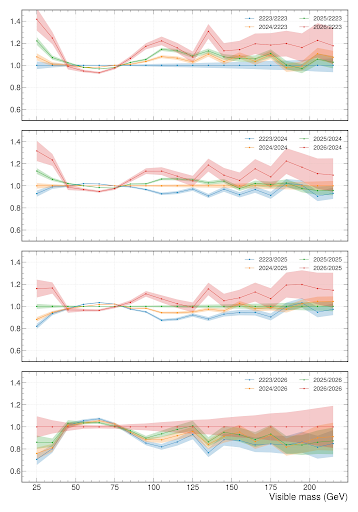
\includegraphics[width=0.5\linewidth]{figures//chapter_III/ratio_DY_2026.png}
    \caption{Ratio of the visible mass $m_{vis}$ distribution in a DY-enriched region across different Run-3 years, shown with respect to a common reference year: the years 2022 and 2023 have been merged as indicated in the figure as 2223 in blue; 2024 in orange; 2025 in blue and 2026 in red. Each panel corresponds to a different reference year, illustrating the evolution of the $m_{vis}$ shape in data between 2022 and 2026. All distributions are normalized to unit area to highlight shape differences only}
    \label{fig:placeholder_2}
\end{figure}

In this way, stability across periods has been verified to account for possible changes in the relative $\tau$ efficiencies, fake rates, and energy scale over the four considered eras. It has been observed that the regions most affected by the different data-acquisition conditions correspond to those dominated by fake $\tau_h$, suchs as events outside the $Z$ mass peak in the DY-enriched region. This indicates that the observed trends stem from variations in the composition and reconstruction of jets misidentified as $\tau_h$ particles, due to detector degradation. Conversely, the response of the detector to authentic hadronic $\tau$ particles remains consistent, validating the stability of the $\tau_h$ energy scale and the efficacy of the reconstruction process throughout the Run-3.

Overall, these stability tests confirm that the performance of the $\tau_h$ in data collected by the detector remains under control across Run-3, with minor variations consistent with the evolution of the detector. This provides an important cross-check of the robustness of the Run-3 $\tau_h$ program.


\vspace{1cm}
\noindent This chapter has demonstrated how the HPS reconstruction and the various identification algorithms — \textsc{DeepTau v2.5}, \textsc{PNet} and \textsc{UParT} — enable the successful identification of the hadronic $\tau$ lepton in experimental collision processes. The focus has been on the various strategies available in CMS, and how the evolution of advanced machine learning techniques, as well as the combination of several of them, enables optimal results to be achieved in discriminating hadronic $\tau$ leptons from various sources of misidentification, while maintaining efficiency for genuine $\tau$ leptons. In addition, the thorough validation process using Run-3 data against Monte Carlo simulations demonstrates the resilience of these algorithms performance under actual detector operating conditions, ensuring reliable and consistent modeling across multiple years. The robustness and confidence provided by the $\tau_h$ program are of great importance for complex physical analyses in final states involving $\tau$ leptons. These elements constitute a fundamental pillar for the study of the $HH\to bb\tau\tau$ channel, which will be discussed in the following chapters.




% Detector holes and hot spots: 
%12.11: https://docs.google.com/presentation/d/15kgMVrNrKn0yoJj5-_G3UvikWLJfFWmZJNiFpdS78qM/edit?slide=id.g2efef749de5_0_3#slide=id.g2efef749de5_0_3
%14.11: https://docs.google.com/presentation/d/1QhgSYqi7aXfBuPNexaYMP5Ko8vo1gtmiUA7vDJvCMOY/edit?slide=id.g3146a045dda_0_0#slide=id.g3146a045dda_0_0
  \part{The bbtt analysis}
\chapter{Tau identification and validation}
  \chapter{The HH-BTag and VBFjTag}


Intro / Motivation / Contexto dentro del analisis bbtautau / uso en Run-2 y Run-3; desarrollo del VBFjTag para Run-3
0) Phenomenology
1) Model: algunos technical details
1.1) Architecture  (same for both taggers) and training; 
1.2) event selection and truth gen definitions (different for each tagger)
1.3) output
2) Input features (dividido en HHBtag / VBfjettag)
2.1) studies on the input features
2.1) feature importance after the training
3) Performance en el analisis
3.1) purity definition as performance evaluation 
3.2) resultados
  \part{The bbtt analysis}
\chapter{bb\texorpdfstring{$\tau\tau$}{ττ} analysis setup}
\section{algo de ZZ/ZH validation?}

  \part{Di-Higgs production beyond the Standard Model}
  
FALTARIA HACER CLARA LA DISTINCION ENTRE LOS DOS CAPITULOS EN SU SITIO CORRESPONDIENTE
\chapter{Results and combination with the Run-2 data set}
\label{ch:bbtt_results}



\section{Statistical procedure}
\label{sec:bbtt_statistics}


\begin{table}[tbp]
\centering
\small
\begin{tabular}{lllc}
\toprule
Source & Affected processes & Type & Correlation across periods \\
\midrule
Integrated luminosity                     & simulated              & normalization & partial \\
Signal cross section                      & signal                 & normalization & full    \\
Background cross sections                 & simulated              & normalization & full    \\
Branching fractions                       & with a Higgs boson     & normalization & full    \\
$b\bar{b}H$ normalization                 & $b\bar{b}H$            & normalization & full    \\
\midrule
Pile-up reweighting                       & simulated              & shape & full    \\
Trigger efficiency                        & simulated              & shape & none    \\
Muon and electron identification and isolation & simulated         & shape & full    \\
Electron energy scale and resolution      & simulated              & shape & full    \\
$\tau_h$ identification                   & simulated              & shape & mixed   \\
$\tau_h$ energy scale                     & simulated              & shape & none    \\
Jet energy scale                          & simulated              & shape & mixed   \\
Jet energy resolution                     & simulated              & shape & none    \\
$b$ tagging                               & simulated              & shape & mixed   \\
Acceptance (QCD scale and PDF)            & simulated              & shape & full    \\
\midrule
Drell--Yan correction, fit                & Drell--Yan             & shape & full    \\
Drell--Yan correction, statistical        & Drell--Yan             & shape & none    \\
Top quark $p_T$ reweighting               & $t\bar{t}$             & shape & full    \\
\midrule
Fake factor envelopes                     & \textit{fakes}         & shape & full    \\
Fake factor statistics                    & \textit{fakes}         & shape & none    \\
Template region statistics                & \textit{fakes}         & shape & none    \\
\midrule
Size of the simulated samples             & simulated              & shape & none    \\
\bottomrule
\end{tabular}
\caption[Summary of the systematic uncertainties]{%
    Summary of the sources of systematic uncertainty considered in the analysis, with the
    processes they affect, whether they modify only the normalization or also the shape of
    the distributions, and their correlation across data-taking periods.}
\label{tab:systematics_summary}
\end{table}


% Placed before the results, as in Jaime's thesis, so the results section can be
% read without interruption.

\subsection{The likelihood model}
% Binned maximum-likelihood fit over the 10 SRs x 5 data-taking periods,
% performed simultaneously. COMBINE / RooFit / RooStats.
% -> code: LimitsArea/, scripts/NBAtoInferenceDatacardsParser.py

\subsection{Observed and expected limits}
% Profile likelihood ratio test statistic; asymptotic modified frequentist CLs.
% Parameters of interest: mu, sigma(HH), or the coupling modifiers.

\subsection{Nuisance parameters}
% Normalisation vs shape uncertainties; correlation scheme across periods
% and across processes.

\section{Results}
\label{sec:bbtt_results}

\subsection{Post-fit distributions}
% DNN scores in the 10 SRs after the fit; show 2024 as the representative period
% (largest L_int), noting the others behave similarly.

\subsection{Signal strength and significance}
% mu = 2.6 +2.1 -1.7 ; observed (expected) significance 1.5 (0.7) sigma.
% No significant excess over the background-only hypothesis.

\subsection{Upper limits on the HH production cross section}
% Per category and combined:
%   inclusive ggHH+qqHH : 6.6 (3.9) x SM   -- resolved 2b drives it
%   qqHH only           : 81 (85)  x SM    -- VBF category drives it
% Per-year breakdown (Table 3): 2022 -> 17 (11), 2023 -> 8 (11), 2024 -> 8.3 (4.4).
% Explain why 2024 dominates: luminosity, new triggers, UParT.

\subsection{Constraints on the Higgs boson couplings}
%   -4.1 < kappa_lambda < 11.2  (expected -2.2 < kappa_lambda < 9.2)
%   -0.2 < kappa_2V < 2.3       (expected -0.2 < kappa_2V < 2.4)

\section{Combination with the Run-2 data set}
\label{sec:bbtt_combination}
% (3) RUN 2 ENTERS HERE, at datacard level.

\subsection{Combination procedure}
% Combined with the published Run-2 search in the same final state
% \cite{CMS-HIG-20-010}: 138/fb at 13 TeV -> 310/fb in total.
% - Some Run-2 theory uncertainties were updated after publication (an extra
%   uncertainty on heavy-flavour associated single-H production), so the standalone
%   Run-2 result differs slightly from the published one -- say this explicitly.
% - Correlation scheme: theory uncertainties (branching ratios, PDF, alpha_s,
%   scales, and notably the joint QCD+m_top uncertainty in ggHH) correlated across
%   Runs; all experimental uncertainties uncorrelated, because detector conditions
%   and calibrations differ.
% - The likelihood is the union of all binned shapes from both analyses; the
%   coupling parametrisation follows the same matrix-inversion method in both.

\subsection{Combined results}
% mu = 0.9 +1.6 -1.4 ; observed (expected) significance 0.7 (0.8) sigma.
%   inclusive : 4.0 (3.0) x SM   [Run 2 alone 3.5 (5.3) ; Run 3 alone 6.6 (3.9)]
%   qqHH only : 62 (70)  x SM
%   -2.5 < kappa_lambda < 9.4  (expected -1.5 < kappa_lambda < 8.4)
%   0.02 < kappa_2V < 2.1      (expected -0.1 < kappa_2V < 2.2)
% 2D exclusion in the kappa_2V - kappa_lambda plane, best fit at (7.1, 0.6).
% Worth a comment: Run 3 observed is weaker than expected while Run 2 is stronger
% than expected -- explain how the two combine rather than leaving it unremarked.

\section{Comparison with other HH searches}
\label{sec:bbtt_comparison}
% Borrowed from Jaime (his Sec. 5.5), and it earns its place.
% CMS Run-2 combination 3.4 (2.5); ATLAS 2.9 (2.4); ATLAS+CMS 2.5 (1.7 / 2.8);
% ATLAS bbtautau with 196/fb -> 5.3 (2.4 / 2.8). Where bbtautau sits among
% bbgammagamma, bbbb and bbWW.

\begin{table}[t]
\centering
\begin{tabular}{llccccl}
\toprule
 & Dataset & $\mathcal{L}$ [fb$^{-1}$] & Obs. & Exp. & Exp.$^{\dagger}$ & Source \\
\midrule
\multirow{3}{*}{CMS}
  & Run 2 (2016--2018)         & 138 & 3.5 & 5.3 & 5.30 & \cite{CMS-PAS-HIG-25-008} \\
  & Run 3 (2022--2024)         & 172 & 6.6 & 3.9 & 4.35 & \cite{CMS-PAS-HIG-25-008} \\
  & Run 2 + Run 3              & 310 & 4.0 & 3.0 & 4.50 & \cite{CMS-PAS-HIG-25-008} \\
\midrule
\multirow{4}{*}{ATLAS}
  & Run 2, original            & 140 & 5.9 & 3.3 & 3.32 & \cite{ATLAS-HH-bbtautau-Run2} \\
  & Run 2, reanalysed          & 140 & 5.4 & 2.6 & 2.62 & \cite{ATLAS-HH-bbtautau-Run3} \\
  & Run 3 (2022--2023)         &  56 & 7.9 & 4.3 & 2.74 & \cite{ATLAS-HH-bbtautau-Run3} \\
  & Run 2 + Run 3              & 196 & 5.3 & 2.4 & 2.86 & \cite{ATLAS-HH-bbtautau-Run3} \\
\bottomrule
\end{tabular}
\caption[Comparison of CMS and ATLAS upper limits in HH $\to$ bb$\tau\tau$]{%
Observed and expected 95\% CL upper limits on the inclusive HH production cross
section relative to the SM prediction, in the bb$\tau\tau$ final state. Expected
limits are quoted under the background-only ($\mu = 0$) hypothesis. The CMS
entries are the inclusive ggHH\,$+$\,qqHH limits of Table~3 of
Ref.~\cite{CMS-PAS-HIG-25-008}; the ATLAS Run~3 entries are those of Table~4 of
Ref.~\cite{ATLAS-HH-bbtautau-Run3}, where ``reanalysed'' denotes the same Run~2
dataset processed with the improved Run~3 analysis, to be compared with the
originally published result of Ref.~\cite{ATLAS-HH-bbtautau-Run2}.
$^{\dagger}$Expected limit rescaled to a common integrated luminosity of
138~fb$^{-1}$ as $\mu\sqrt{\mathcal{L}/138~\mathrm{fb}^{-1}}$, i.e.\ assuming
purely statistical scaling; this column is derived here and is not quoted in the
references. Note that the two Run~3 datasets are not equivalent, as the ATLAS
result does not yet include the 2024 data-taking period.}
\label{tab:hh_bbtautau_limits}
\end{table}

\section{Summary and outlook}
\label{sec:bbtt_summary}
% Each of the reference theses closes its analysis chapter with a summary.
% - What was measured and with what sensitivity.
% - What limits it now: statistically dominated (74%), fake factors the leading
%   experimental systematic (25%).
% - The impact of the Chapter \ref{ch:taggers} algorithms on this result -- this is
%   where the thesis closes its own loop.
% - Outlook: remaining Run-3 luminosity, then HL-LHC.
SE ME HACE UN CAPITULO MUY LARGO (HAY 14 SECCIONES...) SE PUEDE SEPARAR EN VARIOS CAPITULOS? HACIENDOLO UNA "PARTE". ALGO COMO LO QUE TIENE JAIME? TENDRÍA SENTIDO ESA SEPARACION?


\chapter{Results and combination with the Run-2 data set}
\label{ch:bbtt_results_chapter}
% Entradilla: recuperar el hilo del capítulo anterior en dos o tres frases.
% Construida la predicción, comprobada frente a los datos y definido el
% discriminante, queda someterlo al contraste estadístico y extraer la medida.


\section{The statistical model of the search}
\label{sec:bbtt_statistics}
% SOLO lo propio de este análisis. El marco general -- verosimilitud, parámetros
% de estorbo y sus términos de restricción, cociente de verosimilitudes perfilado,
% CLs -- está en la Sección \ref{sec:stat_framework} del Capítulo III.
%
% 1) El ajuste: binado, de máxima verosimilitud, simultáneo sobre las diez
%    categorías x cinco periodos = cincuenta regiones de señal (Sección \ref{sec:bbtt_flow}).
%    Observable en cada una: la salida de la DNN de la Sección \ref{sec:bbtt_extraction},
%    con el binado adaptativo allí descrito.
% 2) Parámetro de interés: la intensidad de señal. Para las interpretaciones en
%    kappa_lambda y kappa_2V, el modelo que parametriza la dependencia de la
%    sección eficaz y de la cinemática (mismo método de inversión de matriz de
%    la Sección \ref{sec:bbtt_samples}).
% 3) Los parámetros de estorbo y su correlación: aquí va la Tabla
%    \ref{tab:systematics_summary}, que ahora está en el Capítulo VI.
%    Correlación entre periodos, y descorrelación por categoría y canal de
%    CMS_FF_stat y CMS_FF_template_stat.
% 4) La estadística de las muestras simuladas: el párrafo de autoMCStats
%    (umbral de diez sucesos efectivos, un parámetro por intervalo compartido
%    por encima y uno por proceso por debajo, n_eff = (sum w)^2 / sum w^2).
% -> code: LimitsArea/, scripts/NBAtoInferenceDatacardsParser.py,
%    config/run3_base_config.py (alias, syst_runPeriod_tag),
%    LimitsArea/scripts/SymmetriseAndSmoothShapes.py (renombrado de nuisances)
%
% MOVER AQUÍ la Tabla tab:systematics_summary desde el Capítulo VI.


\section{Results}
\label{sec:bbtt_results}

\subsection{Post-fit distributions}

\subsection{Signal strength and significance}

\subsection{Impact of the systematic uncertainties}
\label{subsec:bbtt_impacts}
% Prometido desde la entradilla de las sistemáticas (Cap. VI, l. 984).
% - Desglose por familia: Tabla 2 del PAS. Estadística total 74%; fake factors 25%;
%   etiquetado de b 10%; leptones y disparo 9%; energía de jets 7%; otras 3%;
%   teóricas HH 31%, single-H 27%, fondos 14%; variaciones intervalo a intervalo 35%.
%   Decir que se combinan en cuadratura y que por eso no suman 100%.
% - Pull and impact: ordena parámetros individuales por Delta(mu); complementa
%   la tabla, que ordena familias enteras.
% -> code: LimitsArea/scripts/run_syst_breakdown.sh (grupos theoHH, theoH,
%    theoAcc, theoB y las rgx por objeto)

\subsection{Upper limits on the HH production cross section}

\subsection{Constraints on the Higgs boson couplings}


\section{Combination with the Run-2 data set}
\label{sec:bbtt_combination}

\subsection{Combination procedure}

\subsection{Combined results}


\section{Comparison with other HH searches}
\label{sec:bbtt_comparison}


\section{Summary and outlook}
\label{sec:bbtt_summary}



% This ensures that the subsequent sections are being included as root
% items in the bookmark structure of your PDF reader.
\bookmarksetup{startatroot}
\backmatter

  \addchap{Conclusions}
\label{ch:conclusions}
%


  \begin{otherlanguage}{spanish}
\addchap{Conclusiones}
\label{ch:conclusiones}
%

\end{otherlanguage}


  \printbibliography

\end{document}
